% ******************* PhD Thesis Presentation Template *************************
% Please have a look at the README.md file for info on how to use the template
\PassOptionsToPackage{table}{xcolor} % <-μονο εδω δουλεύει!!

\documentclass[customfont, aspectratio=169, printbib]{Classes/beamerPub}%%  
% ******************************************************************************
% ******************************* Class Options ********************************
% *********************** See README for more details **************************
% ******************************************************************************
%
% `aspectratio=169`: reduce ratio to 16:9
%
% `customfont`: Pre-defined font is "Biolinum O". This option enable custom fonts .
% Config custom fonts at `preamble.tex`. Custom font include GFS package.
%
% `10pt` or `11pt`(default) : Recommended font size. Smaller (`8pt`,`9pt`)
% or huge (`14pt`,`17pt`,`20pt`) font size are NOT recommended except special cases.
%
% `draft`: Special draft mode with line numbers, images, and water mark with 
% timestamp and custom text. Position of the text can also be modified. To 
% disable figures see on `preample.tex` the Draftmode section.
%
% `chapter`: This option enables only the specified chapter and it's references
% Useful for review and corrections.
%
% `notes`: Prints frames and notes 
%
% `notes=only`: Prints only notes of each frame
%
% `printbib`: Include bibliography at the end of the presentation 
%
% `progrbar`: Enable progress bar in the frame. Chose this option after your 
% first compilation. Disable on chapter mode.

% ********************************** Preamble **********************************
% Preamble: Contains packages and user-defined commands and settings
% ********************************** Preamble **********************************
% Preamble: Contains packages and user-defined commands and settings
%%-----------------------------------------------------------------------------
%% USE THEME
%%-----------------------------------------------------------------------------
\usetheme{BluePub}
% \usetheme{PaloAlto} 
% \usetheme{Singapore}
% \usetheme{Szeged}
% \usetheme{CambridgeUS}
% \usetheme{Montpellier}
% \usetheme{Pittsburgh} <---
% \usetheme{Warsaw}
% \usetheme{Rochester}
% \usetheme{Marburg}
% \usetheme{Malmoe}
% \usetheme{Madrid}
% \usetheme{Luebeck}
% \usetheme{Ilmenau}
% \usetheme{Hannover} <---
% \usetheme{Goettingen}
% \usetheme{Dresden}
% \usetheme{boxes}
% \usetheme{Boadilla}
% \usetheme{Berlin}
% \usetheme{Berkeley}
% \usetheme{AnnArbor}

\usepackage{lmodern}
\usepackage[scale=2]{ccicons}

%%-----------------------------------------------------------------------------
%%  remove dots from miniframe theme
%%-----------------------------------------------------------------------------
\makeatletter
\def\beamer@writeslidentry{\clearpage\beamer@notesactions}
\makeatother

%%-----------------------------------------------------------------------------
%%  double slides left presentation // right notes NOT WORK WELL!!!
%%-----------------------------------------------------------------------------
% \usepackage{pgfpages}
% \setbeameroption{show notes on second screen=right}

%%-----------------------------------------------------------------------------
%%  margins
%%-----------------------------------------------------------------------------
\setbeamersize{text margin left=0.4cm}  % <- like this
\setbeamersize{text margin right=0.4cm} % <- like this

%%-----------------------------------------------------------------------------
%% Set background for simpledso theme
%%-----------------------------------------------------------------------------
%\graphicspath{{Chapter3/Figs/Vector/}{Chapter3/Figs/}}
\setwatermark{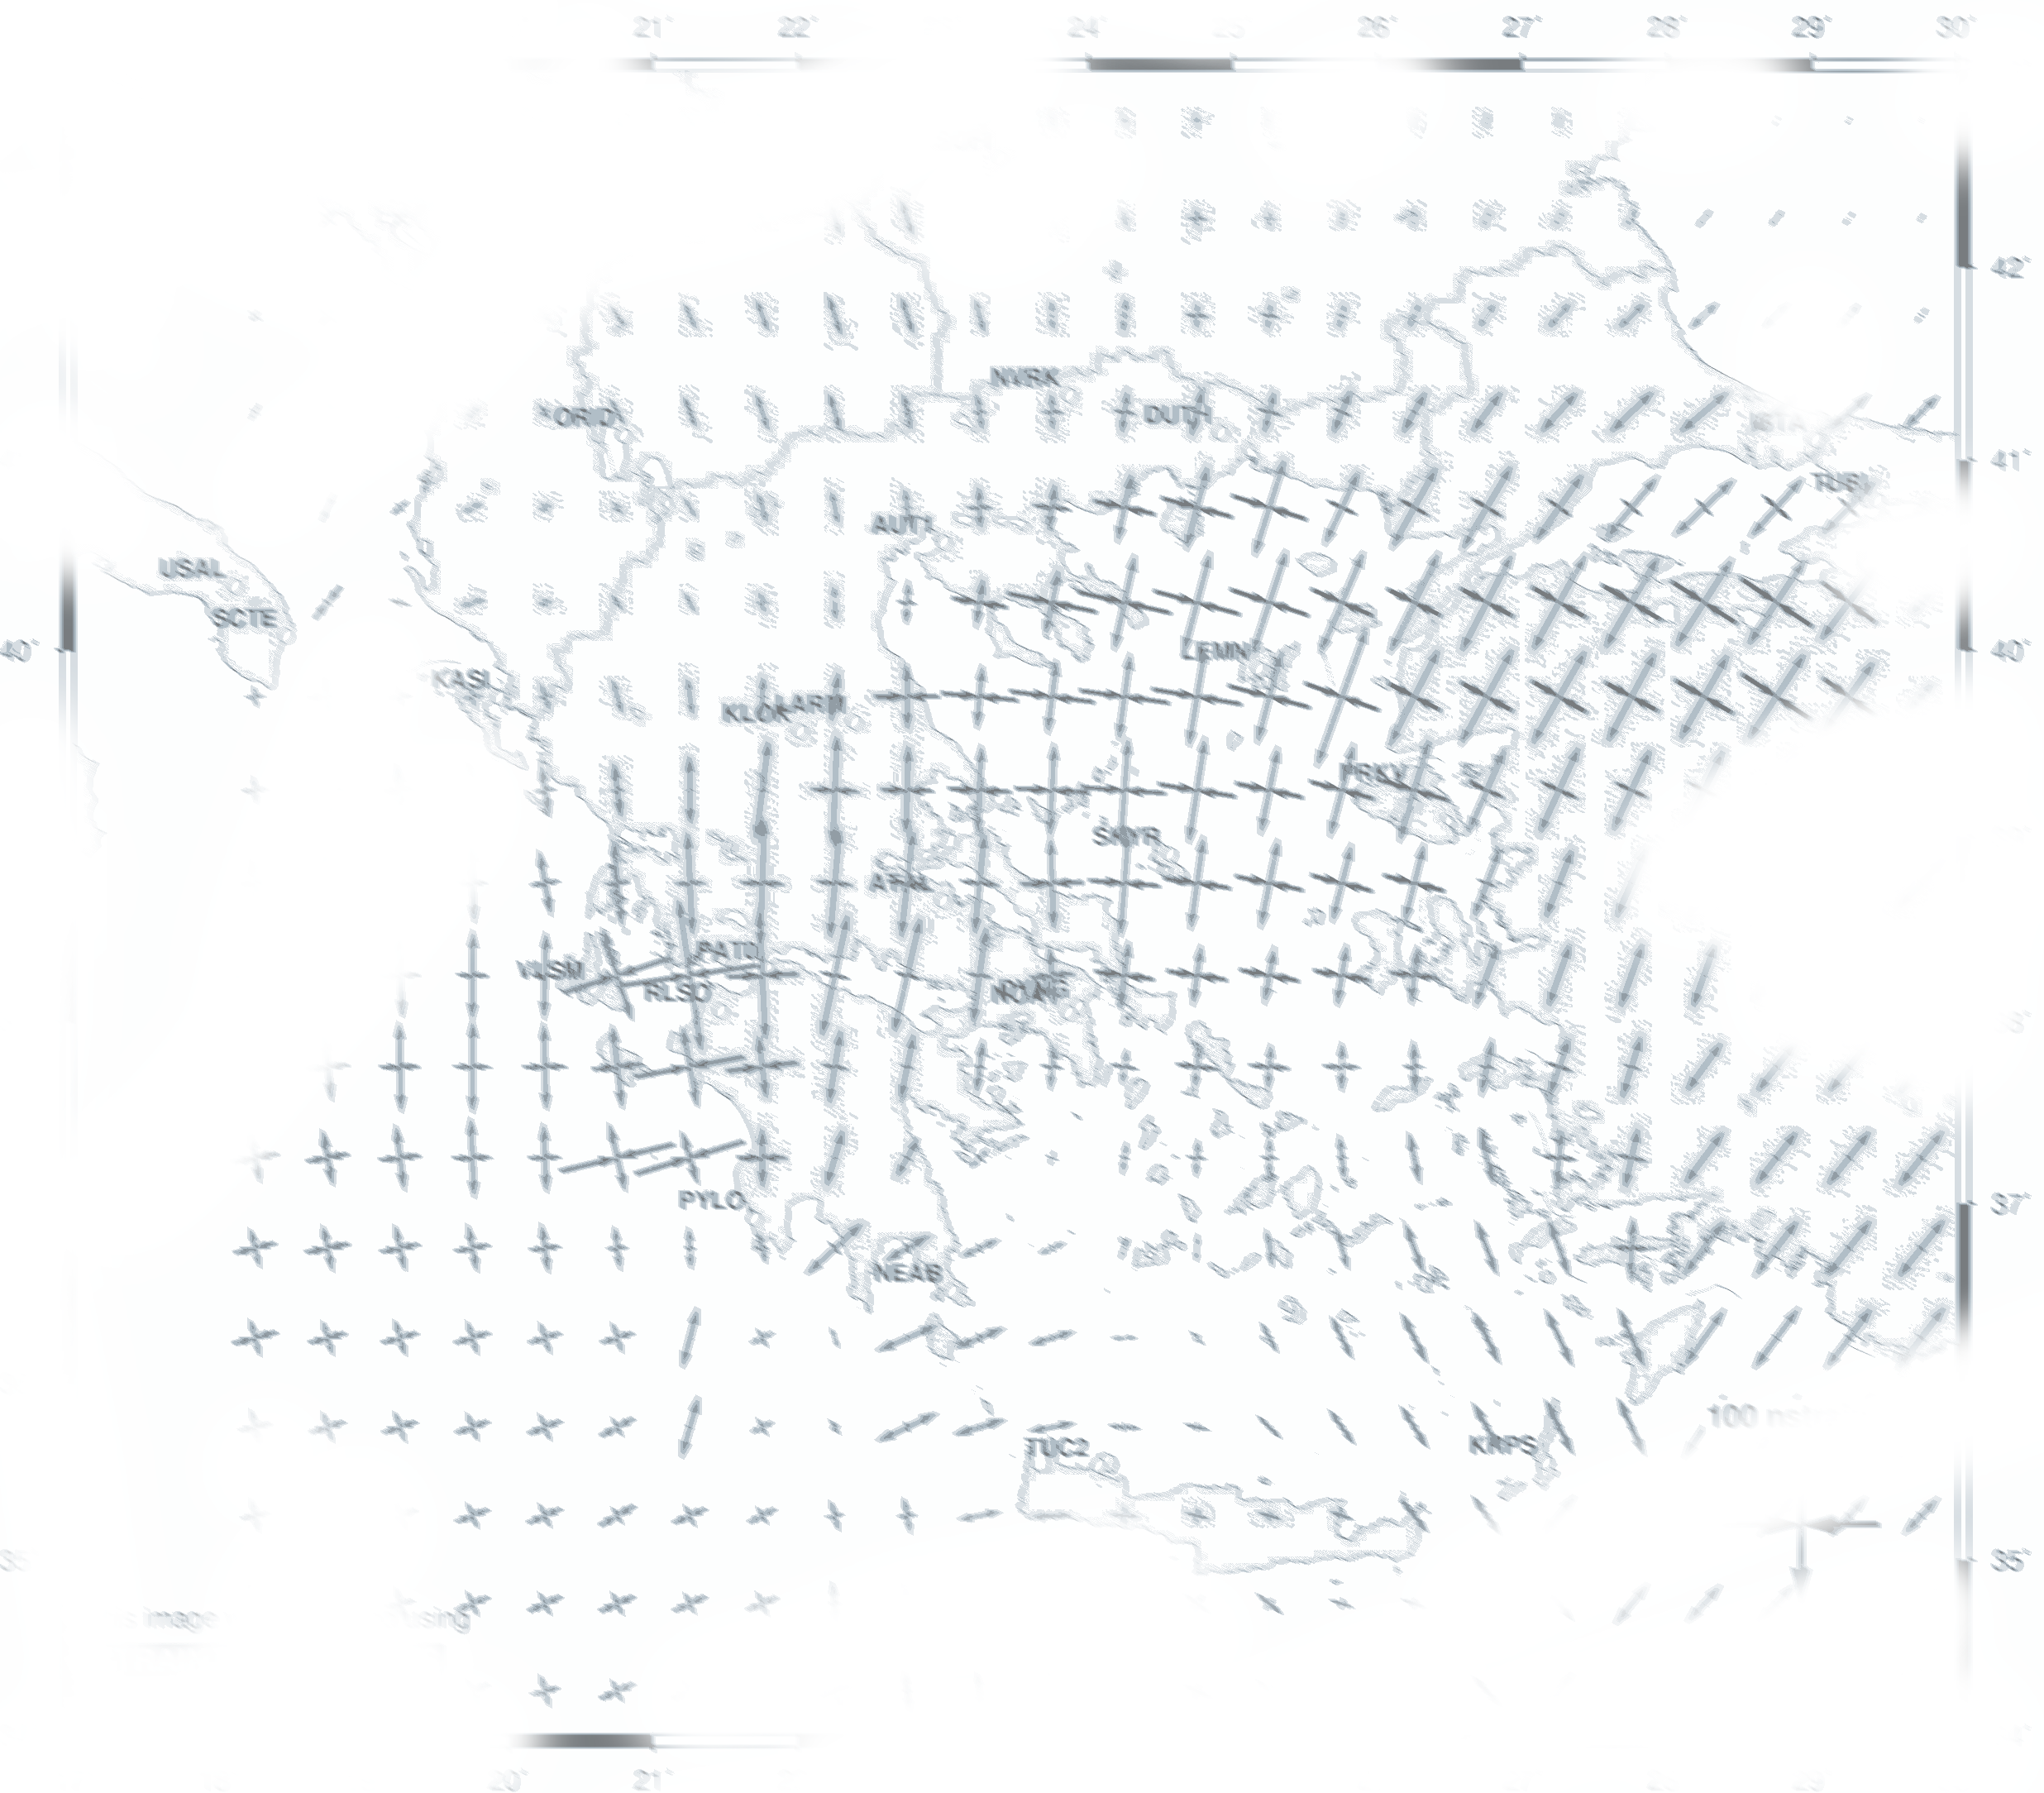
\includegraphics[height=8cm,draft=false]{Figs/back_str.png}}

%%-----------------------------------------------------------------------------
%% Languages
%%-----------------------------------------------------------------------------
% \usepackage[english, greek]{babel}
\usepackage{xgreek}
\usepackage[Greek,Latin]{ucharclasses}
\setTransitionsForGreek{\setlanguage{greek}}{\setlanguage{english}}
% \usepackage{xunicode}
% \usepackage{xltxtra}
% \usepackage[monogreek]{xgreek}
% \usepackage{tabu}

%%-----------------------------------------------------------------------------
%% Tables
%%-----------------------------------------------------------------------------
\usepackage{booktabs,tabularx}
\usepackage{tabu}
\usepackage{multirow}

%%-----------------------------------------------------------------------------
%% Fonts
%%-----------------------------------------------------------------------------

% Add `customfont' in the document class option to use this section
\ifdefineCustomFont
  \usepackage{fontspec}
  \usefonttheme{professionalfonts} % using non standard fonts for beamer
  \usefonttheme{serif} % default family is serif
%  \setmainfont[Mapping=tex-text]{GFS Didot}
%  \setmainfont[Mapping=tex-text]{GFS Bodoni}
%  \setmainfont[Mapping=tex-text]{GFS Olga} % ότι να ναι αυτή!!πλάγια NOT support English
  \setmainfont[Mapping=tex-text]{GFS Neohellenic}
%  \setmainfont[Mapping=tex-text]{GFS Artemisia}
%  \setmainfont[Mapping=tex-text]{GFS Elpis} %low resolution printing


%%  % For use with XeLaTeX, enable Libertine
%    \setmainfont[
%      Path              = /usr/share/texlive/texmf-dist/fonts/opentype/public/libertine/, %./libertine/opentype/,
%      Extension         = .otf,
%      UprightFont = LinLibertine_R,
%      BoldFont = LinLibertine_RZ, % Linux Libertine O Regular Semibold
%      ItalicFont = LinLibertine_RI,
%      BoldItalicFont = LinLibertine_RZI, % Linux Libertine O Regular Semibold Italic
%    ]
%    {LGR}
%  %  % load font from system font
%     \newfontfamily\libertinesystemfont{Linux Libertine O}

%  %% use xetex, enable Biolinum Fonts
%  \setmainfont[
%      Path              = /usr/share/texlive/texmf-dist/fonts/opentype/public/libertine/, %./libertine/opentype/,
%      Extension         = .otf,
%      UprightFont = LinBiolinum_R,
%      BoldFont = LinBiolinum_RB, % Linux Libertine O Regular Semibold
%      ItalicFont = LinBiolinum_RI,
%      %BoldItalicFont = LinBiolinum_RZI, % Linux Libertine O Regular Semibold Italic
%    ]
%    {LGR}
%  %  % load font from system font
%     \newfontfamily\libertinesystemfont{Linux Biolinum O}


\else
  \usepackage{fontspec}
  \usefonttheme{professionalfonts} % using non standard fonts for beamer
  \usefonttheme{serif} % default family is serif

  %% Use Computer Modern Unicode Fonts, Support Greek Font
  \setmainfont[Mapping=tex-text, Scale=0.90]{CMU Serif}
  \setsansfont[Mapping=tex-text, Scale=0.90]{CMU Sans Serif}
  \setmonofont{CMU Typewriter Text}
 
%%************* Latin Modern, not support greek*****************************
%  \usepackage{lmodern}
%  \usepackage[T1]{fontenc}
     
\fi % custom font class

%%-----------------------------------------------------------------------------
%% REQUIRED PACKAGES
%%-----------------------------------------------------------------------------
\usepackage{graphicx}  % Required for including images
\usepackage{fancybox}
% \usepackage{xcolor}
%% for tikz
% \usepackage{dtklogos}
%\usepackage{tikz}
\usetikzlibrary{mindmap,shadows}
\usepackage{smartdiagram}

% restart numbering footnotes per page
\usepackage{perpage}
\MakePerPage{footnote}
% % Sychronize footnotes on columns minipages
\renewcommand\thempfootnote{\arabic{mpfootnote}}

% use nice itemlists ..
%\usepackage{enumitem, color, amssymb}
\usepackage{url}
% \hypersetup{colorlinks,linkcolor=,urlcolor=links}
\hypersetup{colorlinks=true,allcolors=blue}

% use metalogo to print xelatex!
\usepackage{metalogo}

% % tcolorbox custom block, problem with caption package, cant solve it yet!
% \usepackage[most]{tcolorbox}

%%-----------------------------------------------------------------------------
%% Adgust figures
%%-----------------------------------------------------------------------------
\usepackage{adjustbox} % for \adjincludegraphics
% {\shadowbox{\color{black!35}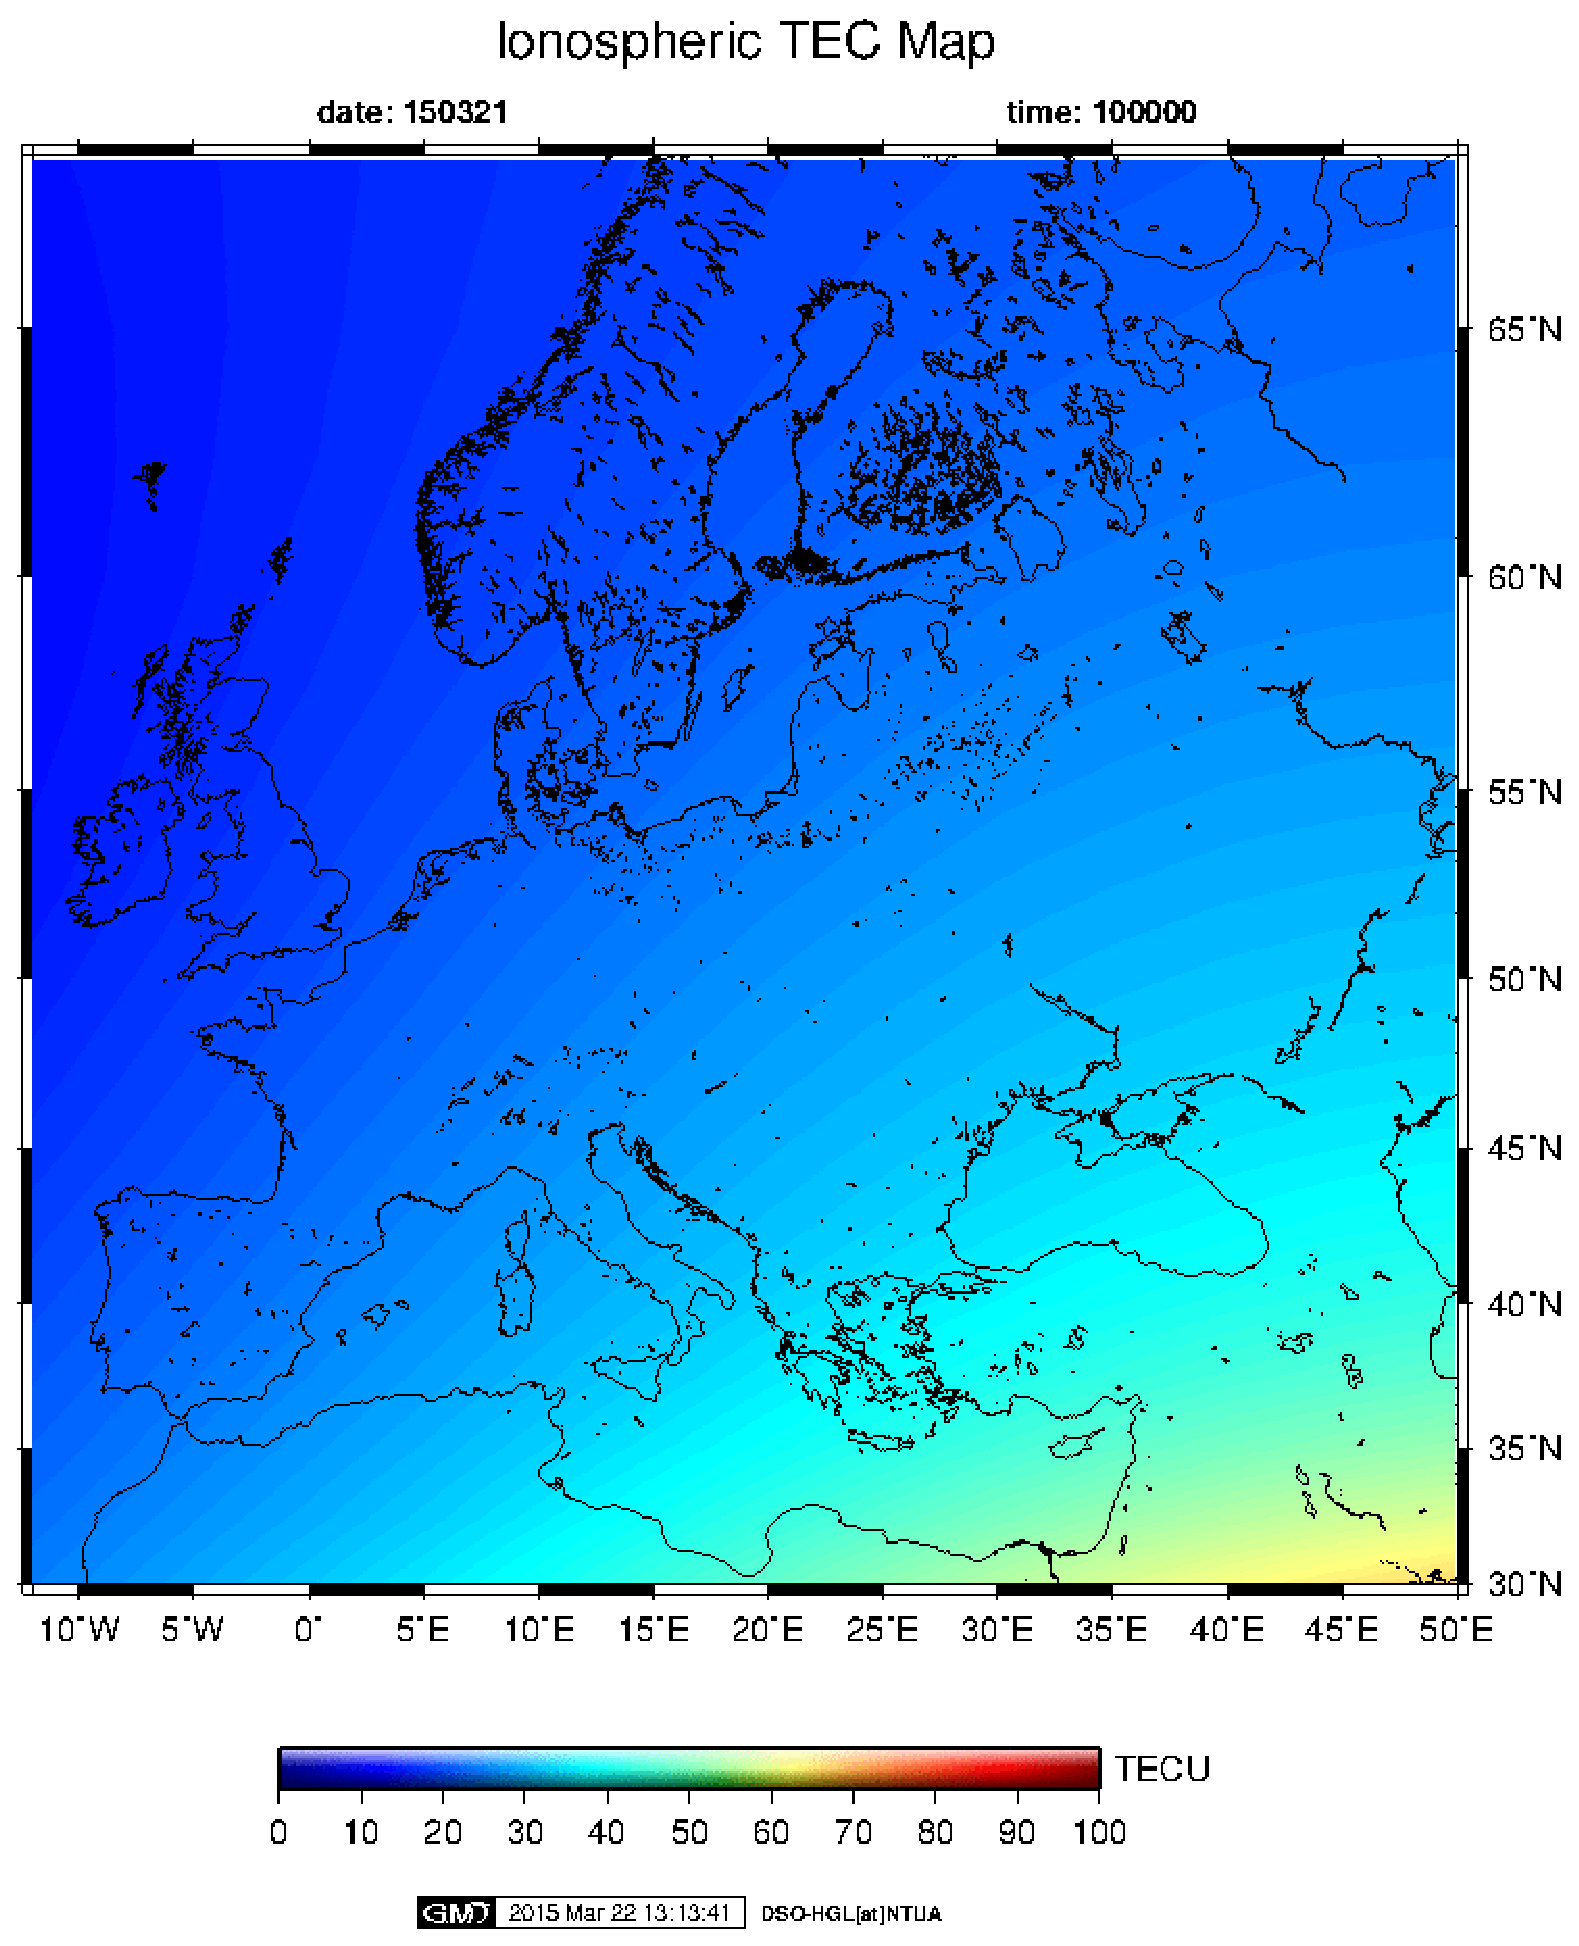
\includegraphics[height=4cm]{img/iono.eps}}

%%-----------------------------------------------------------------------------
%% Print Arrows
%%-----------------------------------------------------------------------------
\usepackage{marvosym} % \MVRIGHTarrow
\usepackage{stmaryrd} % \shortrightarrow $\Rightarrow$
\usepackage{textcomp} % \textrightarrow

%%-----------------------------------------------------------------------------
%% Math symbols
%%-----------------------------------------------------------------------------
\usepackage{amssymb} 
\usepackage{amsmath}

% \usepackage{soul}
% \definecolor{lightblue}{rgb}{.90,.95,1}
% \sethlcolor{lightblue}
% \renewcommand<>{\hl}[1]{\only#2{\beameroriginal{\hl}}{#1}}
% -----------------------------------------------------------------------------
% CAPTIONS
%-----------------------------------------------------------------------------
\usepackage{caption}
\usepackage{subcaption}
\captionsetup[figure]{font=footnotesize,labelfont=footnotesize,skip=0pt,belowskip=0pt}
\setbeamertemplate{caption}[numbered]

\setbeamerfont{caption}{size=\scriptsize}

% -----------------------------------------------------------------------------
% Four Quad
%-----------------------------------------------------------------------------
\newcommand\FourQuad[4]{
    \begin{minipage}[b][.45\textheight][t]{.50\textwidth}\centering#1\end{minipage}\hfill%
    \begin{minipage}[b][.45\textheight][t]{.50\textwidth}\centering#2\end{minipage}\\[0.1cm]
    \begin{minipage}[b][.45\textheight][t]{.50\textwidth}\centering#3\end{minipage}\hfill
    \begin{minipage}[b][.45\textheight][t]{.50\textwidth}\centering#4\end{minipage}%
}

% -----------------------------------------------------------------------------
% Custom symbols for itemize
%-----------------------------------------------------------------------------

\newenvironment{proenv}{\only{\setbeamercolor{local structure}{fg=green}}}{}
\newenvironment{conenv}{\only{\setbeamercolor{local structure}{fg=red}}}{}
 \usepackage{fontawesome}

% -----------------------------------------------------------------------------
% Rotate text
%-----------------------------------------------------------------------------
\usepackage{rotating}
%\begin{turn}{45} 
% ...
% \end{turn}


% -----------------------------------------------------------------------------
% BIBLATEX
%-----------------------------------------------------------------------------
\usepackage{hyperref}
\usepackage[backend=biber,
            style=authoryear,
            maxbibnames=9,
            maxcitenames=1,
            citestyle=authoryear,
            hyperref=true,
            backref=true,
            sorting=nty,
            natbib=true]{biblatex}

% Hypper linc for all citations use \parencite & \textcite
\ExecuteBibliographyOptions{maxcitenames=1}

\DeclareFieldFormat{citehyperref}{%
  \DeclareFieldAlias{bibhyperref}{noformat}% Avoid nested links
  \bibhyperref{#1}}

\DeclareFieldFormat{textcitehyperref}{%
  \DeclareFieldAlias{bibhyperref}{noformat}% Avoid nested links
  \bibhyperref{%
    #1%
    \ifbool{cbx:parens}
      {\bibcloseparen\global\boolfalse{cbx:parens}}
      {}}}

\savebibmacro{cite}
\savebibmacro{textcite}

\renewbibmacro*{cite}{%
  \printtext[citehyperref]{%
    \restorebibmacro{cite}%
    \usebibmacro{cite}}}

\renewbibmacro*{textcite}{%
  \ifboolexpr{
    ( not test {\iffieldundef{prenote}} and
      test {\ifnumequal{\value{citecount}}{1}} )
    or
    ( not test {\iffieldundef{postnote}} and
      test {\ifnumequal{\value{citecount}}{\value{citetotal}}} )
  }
    {\DeclareFieldAlias{textcitehyperref}{noformat}}
    {}%
  \printtext[textcitehyperref]{%
    \restorebibmacro{textcite}%
    \usebibmacro{textcite}}}



\bibliography{References/triangleref.bib}
\newcounter{bibitmctr}
\newcommand{\brf}{%
  \stepcounter{bibitmctr}%
  \ifnum\value{bibitmctr}=7%
    \setcounter{bibitmctr}{0}
    \framebreak
  \fi
}

\renewbibmacro*{finentry}{\finentry\brf}

% % cahnge fontsize of bibliography for biblatex
\renewcommand*{\bibfont}{\tiny}


%%-----------------------------------------------------------------------------
%% Insert frame after new section
%%-----------------------------------------------------------------------------
%%% comment next lines if you don't like to use this
%\AtBeginSection[]{
%  \begin{frame}[b]
%%   \vfill
%  \vspace{\fill}
%  \centering
%  \begin{beamercolorbox}[sep=8pt,center,shadow=true,rounded=true]{title}
%    \usebeamerfont{title}\Large{\insertsection} %
%  \end{beamercolorbox}
%  \vskip-2cm
%  \begin{flushleft}
%    {\color{red!20}\rule{0.7\textwidth}{1pt}}\par
%    {\color{red!40}\rule{0.5\textwidth}{1pt}}\par
%    {\color{red!60}\rule{0.3\textwidth}{1pt}}\par
%    {\color{red!70}\rule{0.16\textwidth}{1pt}}\par
%    {\color{red!80}\rule{0.08\textwidth}{1pt}}\par
%    {\color{red!90}\rule{0.04\textwidth}{1pt}}\par
%  \end{flushleft}
%  \vspace{.5cm}
%%   \vfill
%  \end{frame}
%}

% -----------------------------------------------------------------------------
% Configure Draft mode
%-----------------------------------------------------------------------------
% *********************** Configure Draft Mode **********************************
\ifsetDraft
  \usepackage[printwatermark]{xwatermark}
  % Bottom
  \newwatermark*[pages=2-,color=red!60,textalign=center,angle=0,scale=.37,xpos=-.2cm,ypos=-.437\paperheight]{\makebox[.9\textwidth]{{\drafttext}\space-\space{\draftVersion}\space{\timestamp}}}
  %Flush right
%  \newwatermark*[pages=2-,color=red!60,textalign=center,angle=90,scale=.35,xpos=.45\paperwidth, ypos=-.7cm]{\makebox[.9\textwidth]{{\drafttext}\space-\space{\draftVersion}\space{\timestamp}}}
  
\fi 

% Uncomment to disable figures in `draft' mode
% \setkeys{Gin}{draft=true}  % set draft to false to enable figures in `draft'

% These options are active only during the draft mode
% Default text is "Draft"
\SetDraftText{DRAFT}

% Draft Version - default is v1.0
\SetDraftVersion{v1.0}

% ******************************** Todo Notes **********************************
%% Uncomment the following lines to have todonotes. % Not working yet!

% \ifsetDraft
%   \usepackage[colorinlistoftodos,prependcaption,textsize=small]{todonotes}
%   \setlength{\marginparwidth}{2.2cm}
% % 	\usepackage[colorinlistoftodos]{todonotes}
% 	\newcommand{\mynote}[1]{\todo[author=mitsos,size=\small,inline,color=green!40]{#1}}
%   \newcommand{\unsure}[1]{\todo[author=mitsos,size=\small,color=red!60]{#1}}
% 	\newcommand{\change}[2][1=]{\todo[author=mitsos,size=\small,linecolor=blue,backgroundcolor=blue!35,bordercolor=blue]{#1}}
% % 	\newcommand{\info}[2][1=]{\todo[linecolor=OliveGreen,backgroundcolor=OliveGreen!25,bordercolor=OliveGreen,#1]{#2}}
% % 	\newcommand{\improvement}[2][1=]{\todo[linecolor=Plum,backgroundcolor=Plum!25,bordercolor=Plum,#1]{#2}}
% 	\newcommand{\xanthos}[1]{\todo[author=xanthos,size=\small,inline,color=red!40]{#1}}
% 	\newcommand{\vagg}[1]{\todo[author=vagg,size=\small,inline,color=red!40]{#1}}
% \else
%   \newcommand{\todo}[1]{}
% 	\newcommand{\mynote}[1]{}
% 	\newcommand{\unsure}[1]{}
% 	\newcommand{\change}[1]{}
% 	\newcommand{\info}[2][1=]{}
% 	\newcommand{\improvement}[2][1=]{}
% 	\newcommand{\xanthos}[1]{}
% 	\newcommand{\vagg}[1]{}
% 	\newcommand{\listoftodos}{}
% \fi
%
% Example todo: \mynote{Hey! I have a note}


% ************************ Thesis Information & Meta-data **********************
% Thesis title and author information, refernce file for biblatex
% ************************ Pres Information & Meta-data ************************
% This file includes all available informations and meta-data for your presentation
% in four sections:
% 1. General & contact informations, for all styles.
% 2. PhD: Use this section with PhD style.
% 3. Pub: Use this section with publication style.
% 4. Lct: Usethis section with lecture style.
%
% Uncomment only one section of 2,3 or 4 each time.

%% -----------------------------------------------------------------------------
%% 1.General information... 
%% -----------------------------------------------------------------------------
% ************************ Pres Information & Meta-data ************************

%% Meta information
% \subject{Γεωδαισία} \keywords{{Γεωδαισία} {Τριγωνισμός} {Παραμόρφωση} {Ελλάδα}}

%% Contact e-informations
\urlhome{http://dionysos.survey.ntua.gr/}  %% homepage
\contmail{danastasiou@mail.ntua.gr}  %% contact mail
\urlin{https://www.linkedin.com/in/dganastasiou/}  %% linkedin url
\urlgh{https://github.com/demanasta}  %% github repository
%\urlgp{https://plus.google.com/u/0/+DemitrisAnastasiou}  %% Google+ 
\urltw{https://twitter.com/DemAnast}  %% Twitter

%% Add "thank you" text% 
\thankutext{Ευχαριστούμε για την προσοχή σας!}

% %% -----------------------------------------------------------------------------
% %% 2.PhD section INFO
% %% -----------------------------------------------------------------------------
% %% ************************ Thesis Information & Meta-data **********************
% %% The title of the thesis
% \eltitle{ΠΡΟΤΥΠΟ ΠΑΡΟΥΣΙΑΣΗΣ ΣΕ ΠΑΡΙΒΑΛΛΟΝ \\ Beamer-\LaTeX / \XeLaTeX}
% 
% %% Subtitle (Optional)
% % \subtitle{Using the CUED template}
% 
% %% The full name of the author
% \authorname{ΔΗΜΗΤΡΙΟΣ Γ. ΑΝΑΣΤΑΣΙΟΥ}
% \authortitle{Διπλ. Αγρονόμος \& Τοπογράφος Μηχανικός Ε.Μ.Π}
% 
% %% Department (eg. Department of Engineering, Maths, Physics)
% \dept{ΣΧΟΛΗ ΑΓΡΟΝΟΜΩΝ \& ΤΟΠΟΓΡΑΦΩΝ ΜΗΧΑΝΙΚΩΝ}
% 
% %% Laboratory
% \lab{ΚΕΝΤΡΟ ΔΟΡΥΦΟΡΩΝ ΔΙΟΝΥΣΟΥ}
% 
% %% University and Crest
% \university{ΕΘΝΙΚΟ ΜΕΤΣΟΒΙΟ ΠΟΛΥΤΕΧΝΕΙΟ}
% 
% % Crest minimum should be 30mm.
% \crestleft{
\includegraphics[width=\textwidth,draft=false]{Figs/ntua.png}}
% \crestright{
\includegraphics[width=0.85\textwidth,draft=false]{Figs/DSOtrans.png}}
% 
% %% Full title of the Degree
% \degreetitle{ΔΙΔΑΚΤΟΡΙΚΗ ΔΙΑΤΡΙΒΗ}
% 
% % Supervisor
% \supervisor{......O/E.........\\ ....Θέση..........}
% 
% %% College affiliation (optional)
% \city{ΑΘΗΝΑ}
% 
% %% Submission date
% % Default is set as {\monthname[\the\month]\space\the\year}
% % \degreedate{\today} 
% \degreedate{5 Ιουλίου 2017}



%% -----------------------------------------------------------------------------
%% 3.Publication's section INFO
%% -----------------------------------------------------------------------------
%% The title of the thesis
\prestitle{Υποστήριξη του δικτύου μόνιμων σταθμών GNSS\\ του Ελληνικού Κτηματολογίου\\ Επεξεργασία δεδομένων - Ανάλυση χρονοσειρών θέσης}

%% The team prepare this presentation
\presteam{Μαρία Τσακίρη,
Ξάνθος Παπανικολάου,
Δημήτριος Αναστασίου}

%% Organizations of the team
\presorgn{Κέντρο Δορυφόρων Διονύσου\\ Σχολή Αγρονόμων και Τροπογράφων Μηχανικών - Μηχανικών Γεωπληροφορικής \\ Εθνικό Μετσόβιο Πολυτεχνείο\\
}
%Contact informations
\presweb{dionysos.survey.ntua.gr}  % webpage
\presmail{dso@survey.ntua.gr}  % contact mail

%% Conference details, Select  text or logo type. If you define both only logo will
%% be print
% \confname{12\textsuperscript{th} HSTAM International Congress on Mechanics}
% \confdetail{Thessaloniki, Greece, 22 - 25 September 2019}

%% OR conf logo....
\conflogo{
\begin{minipage}{5cm}
\begin{flushright}
\vskip-1cm
\textit{Διαδικτυακή παρουσίαση}\\
\textbf{Τετάρτη 14 Ιουνίου}\\
\textbf{2023}
\end{flushright}
\end{minipage}

\includegraphics[width=3cm,draft=false]{Figs/ktima_logo.png}}

%% -----------------------------------------------------------------------------
%% 4.Course section INFO
%% -----------------------------------------------------------------------------
% 
% %%% Department (eg. Department of Engineering, Maths, Physics)
% \dept{ΣΧΟΛΗ ΑΓΡΟΝΟΜΩΝ \& ΤΟΠΟΓΡΑΦΩΝ ΜΗΧΑΝΙΚΩΝ}
% 
% %% Laboratory
% \lab{ΚΕΝΤΡΟ ΔΟΡΥΦΟΡΩΝ ΔΙΟΝΥΣΟΥ}
% 
% %% University and Crest
% \university{ΕΘΝΙΚΟ ΜΕΤΣΟΒΙΟ ΠΟΛΥΤΕΧΝΕΙΟ}
% 
% % Crest minimum should be 30mm.
% \crestleft{
\includegraphics[width=\textwidth,draft=false]{Figs/ntua.png}}
% \crestright{
\includegraphics[width=0.85\textwidth,draft=false]{Figs/DSOtrans.png}}
% 
% 
% %% The full name of the author
% \authorname{ΔΗΜΗΤΡΙΟΣ Γ. ΑΝΑΣΤΑΣΙΟΥ}
% \authortitle{Δρ. Αγρ. \& Τοπ. Μηχ. Ε.Μ.Π}
% 
% %% Lecture title
% \coursetitle{Τίτλος του Μαθήματος}
% \courseinfo{5ο Εξάμηνο}
% \lcttitle{Δημιουργία παρουσιάσεων σε περιβάλλον {\LaTeX}}
% 
% 
% %%% College affiliation (optional)
% \city{ΑΘΗΝΑ}
% 
% %% Submission date
% % Default is set as {\monthname[\the\month]\space\the\year}
% % \degreedate{\today} 
% \coursedate{01 Οκτωβρίου 2017}












% ***************************** Chapter Mode ***********************************
\ifdefineChapter
\includeonly{Chapter1/ch1intro}
%\includeonly{Chapter2/ch2pres}
% \includeonly{Chapter3/ch3pres}
% \includeonly{Chapter4/ch4pres}
% \includeonly{Chapter5/ch5pres}
% \includeonly{Chapter6/ch6pres}
% \includeonly{Appendix/ap_refs}
% \includeonly{Appendix/ap_soft}
% \includeonly{Appendix/cut01.tex}
\fi

% ***********************  Start the document  ***********************************
\begin{document}

% *****************************  Make title  *************************************
\maketitle

% *****************************  TOC  *************************************
%\begin{frame}
%  \frametitle{Ενότητες παρουσίασης}
%  \tableofcontents
%\end{frame}


% ************************  Include Chapters  *************************************

\graphicspath{{R250215/Figs/}}

 % ------------------------------------------------------------------------------
\begin{frame}
  \frametitle{Ανάλυση δεδομένων GNSS στο ΚΔΔ}
  \framesubtitle{}
  \label{}
  \begin{columns}[T]
    \begin{column}{.5\textwidth}
    \textbf{Ανάλυση δεδομένων GNSS}
      \begin{itemize}\setlength\itemsep{1em}
         \item Bernese v5.2 / v5.4 \citep{Bernese}
         \item PRIDE-PPPAR \citep{PRIDE}
         \item GipsyX \citep{GipsyX}
       \end{itemize} 
    \textbf{Ανάλυση χρονοσειρών}
    \begin{itemize}\setlength\itemsep{1em}
      \item Hector v2.1 \citep{Bos2012}
      \item Python/C++ routines
    \end{itemize}
    \end{column}
    \begin{column}{.5\textwidth}
      \textbf{Συχνότητα ανάλυσης}
      \begin{itemize}\setlength\itemsep{1em}
        \item Ημερήσιες λύσεις
          \begin{itemize}\setlength\itemsep{1em}
            \item Rapid solution - 1 day after
            \item Final solution - 12 days after
          \end{itemize}
        \item Ανάλυση υψηλών συχνοτήτων (>1Hz)
          \begin{itemize}\setlength\itemsep{1em}
            \item Δεδομένα HEPOS - 1Hz
          \end{itemize}
      \end{itemize}
    \end{column}
  \end{columns}
  \begin{columns}[T]
    \begin{column}{.1\textwidth}
      \begin{center}
        \includegraphics[width=.7\textwidth]{logo_Bernese.png}
      \end{center}
    \end{column}
    \begin{column}{.2\textwidth}
      \begin{center}
        
\includegraphics[width=.97\textwidth]{logo_PRIDE.png}
      \end{center}      
    \end{column}
    \begin{column}{.2\textwidth}
      \begin{center}
        
\includegraphics[width=.8\textwidth]{logo_gipsyX.png}
      \end{center}      
    \end{column}
    \begin{column}{.5\textwidth}
      \begin{center}

      \end{center}      
    \end{column}    
    
  \end{columns}
\end{frame}
\note{}

 % ------------------------------------------------------------------------------
\begin{frame}
  \frametitle{Διαθέσιμοι σταθμοί}
  \framesubtitle{}
  \label{}
  \vskip-1cm
  \begin{columns}[T]
    \begin{column}{.5\textwidth}
      \begin{center}
        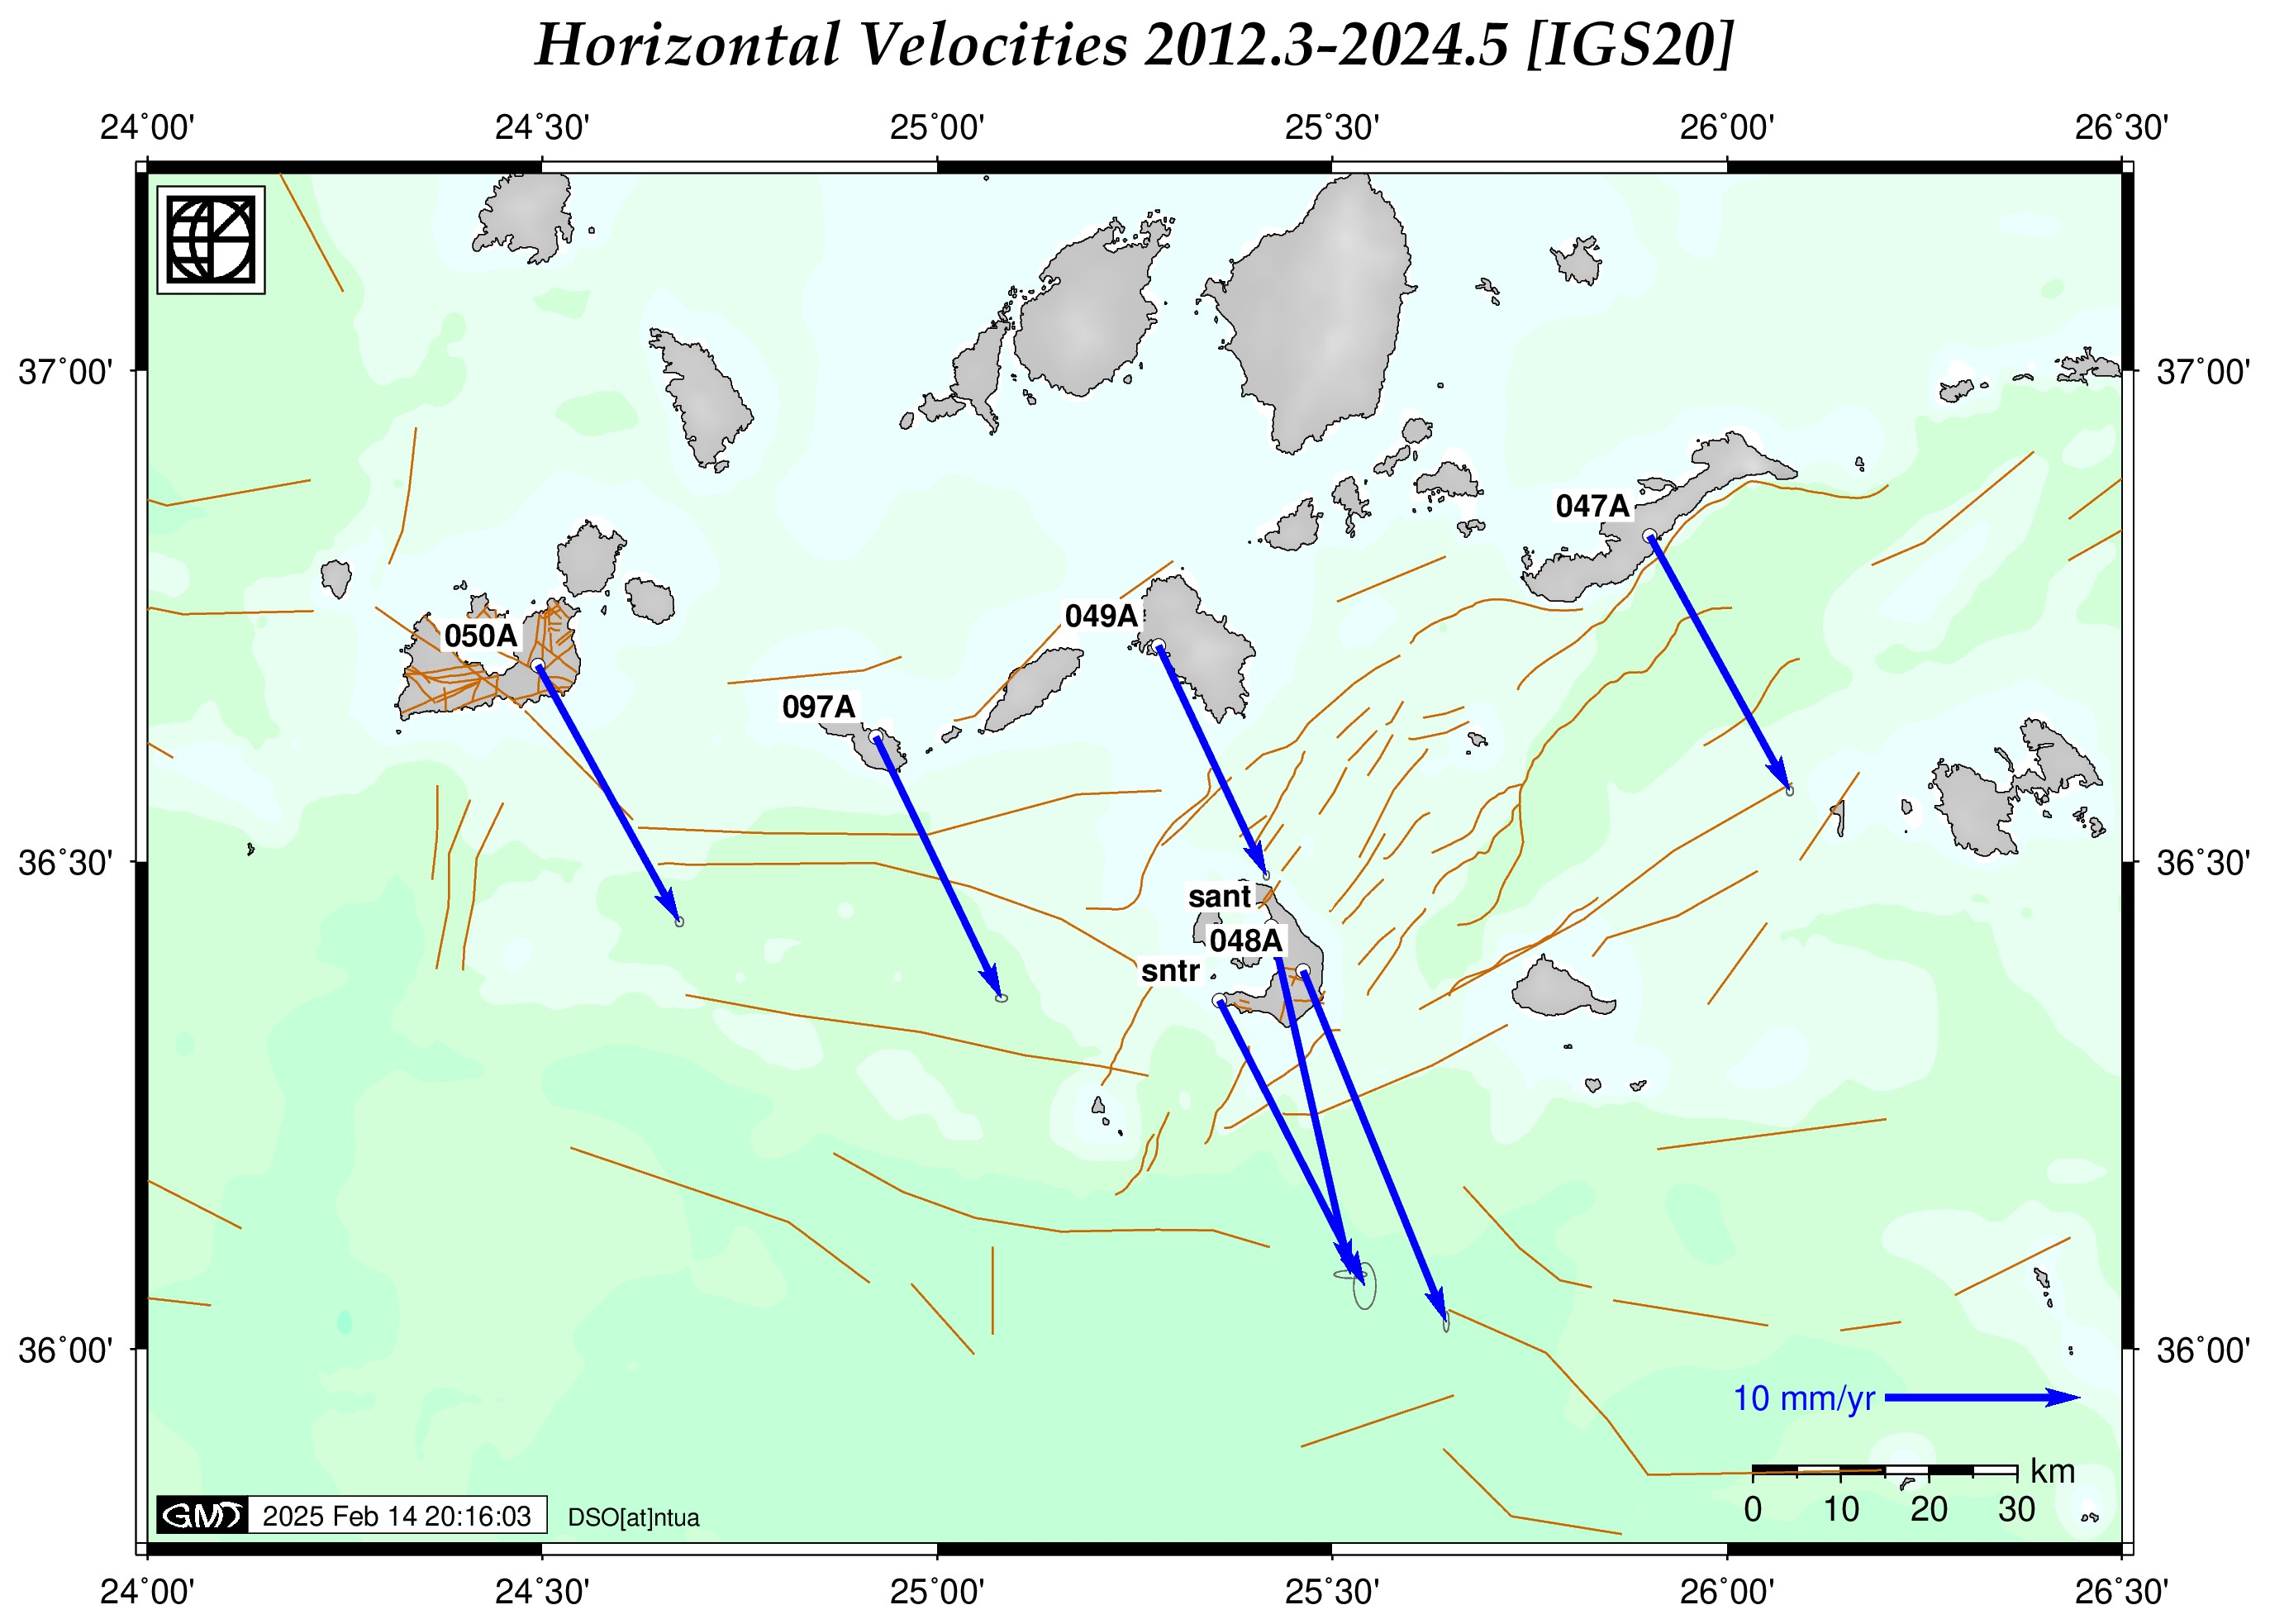
\includegraphics[width=.97\textwidth]{sant_1224_vhor.jpg}
      \end{center}  
    \end{column}
    \begin{column}{.5\textwidth}
      \begin{center}
        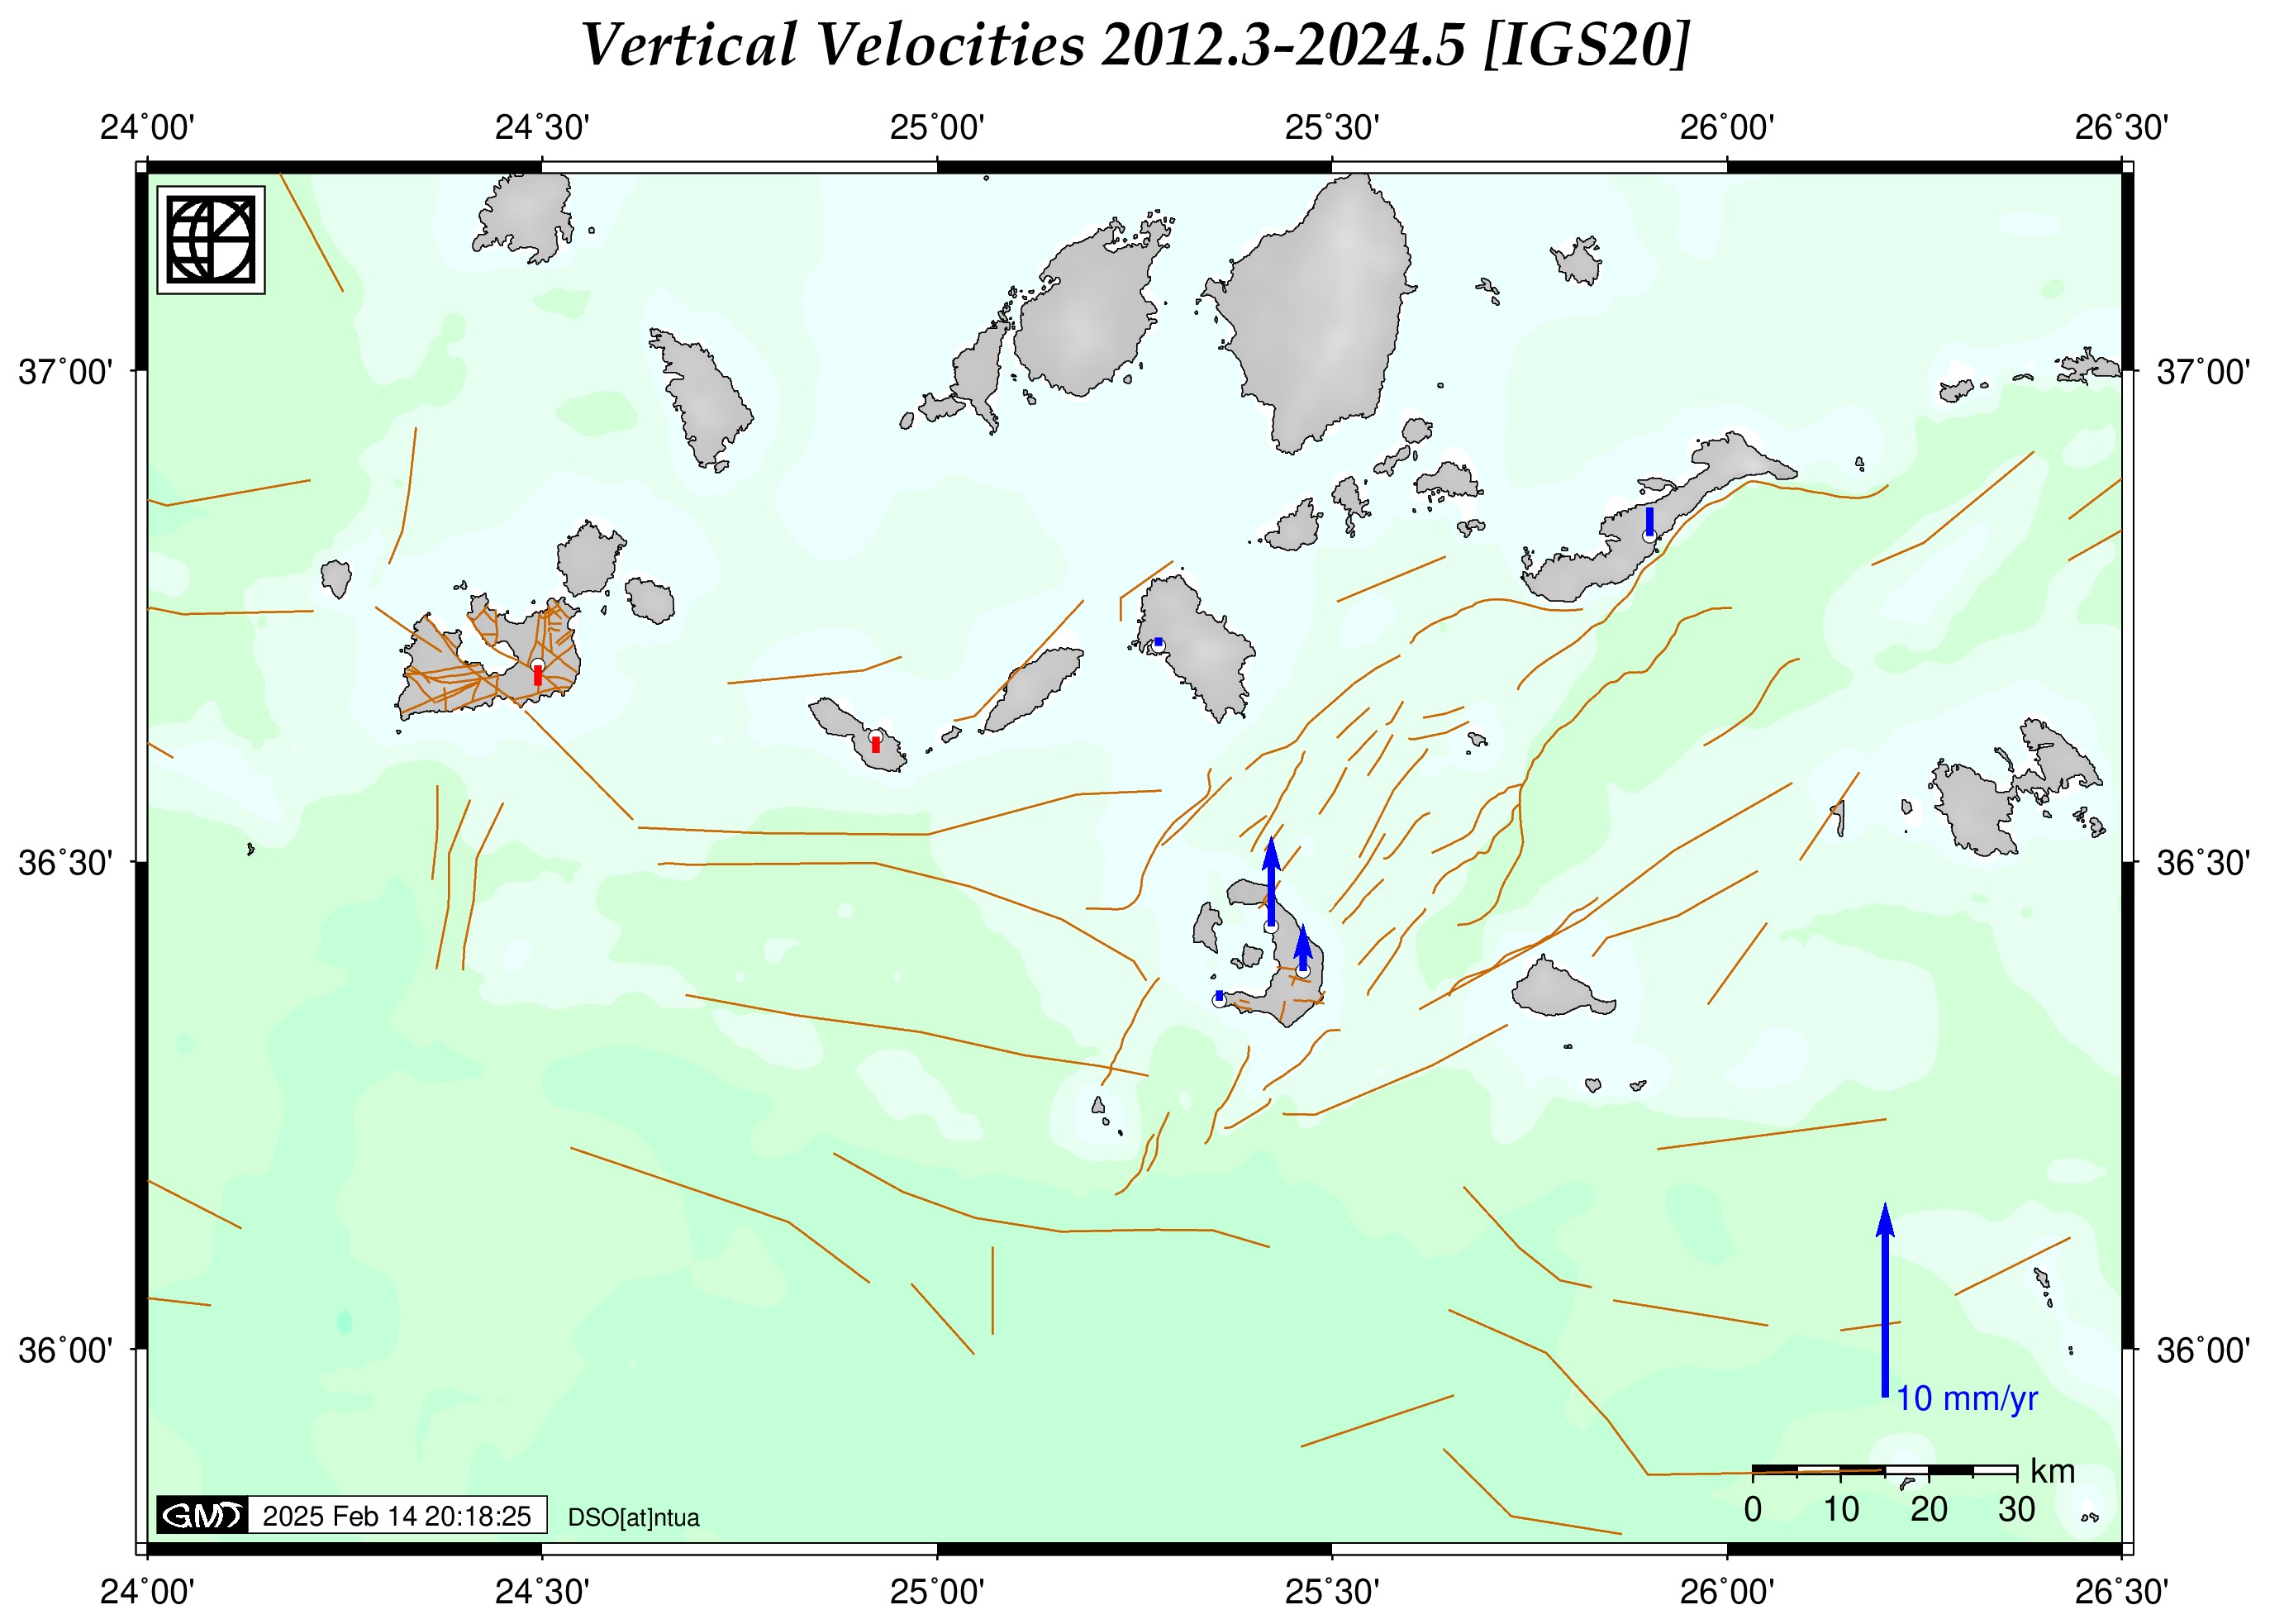
\includegraphics[width=.97\textwidth]{sant_1224_vver.jpg}
      \end{center}       
    \end{column}
  \end{columns}
~\\[1em]   
  \begin{tiny}
  \begin{itemize}\setlength\itemsep{.1em}
    \item[*] Δημιουργία χαρτών: Generic Mapping Tools \citep{gmt}
    \item[*] Υπόβαθρο: ETOPO1 \citep{etopo1}
    \item[*] Βάση ρηγμάτων: NOAfaults v6.0 \citep{noafaults}
  \end{itemize}
  \end{tiny}  
 
\end{frame}
\note{}

 % ------------------------------------------------------------------------------
\begin{frame}
  \frametitle{Ανάλυση χρονοσειρών}
  \framesubtitle{}
  \label{}
  \vskip-1cm
  \begin{columns}[T]
    \begin{column}{.25\textwidth}
      \begin{center}
      {\scriptsize 047A (Αμοργός)}
        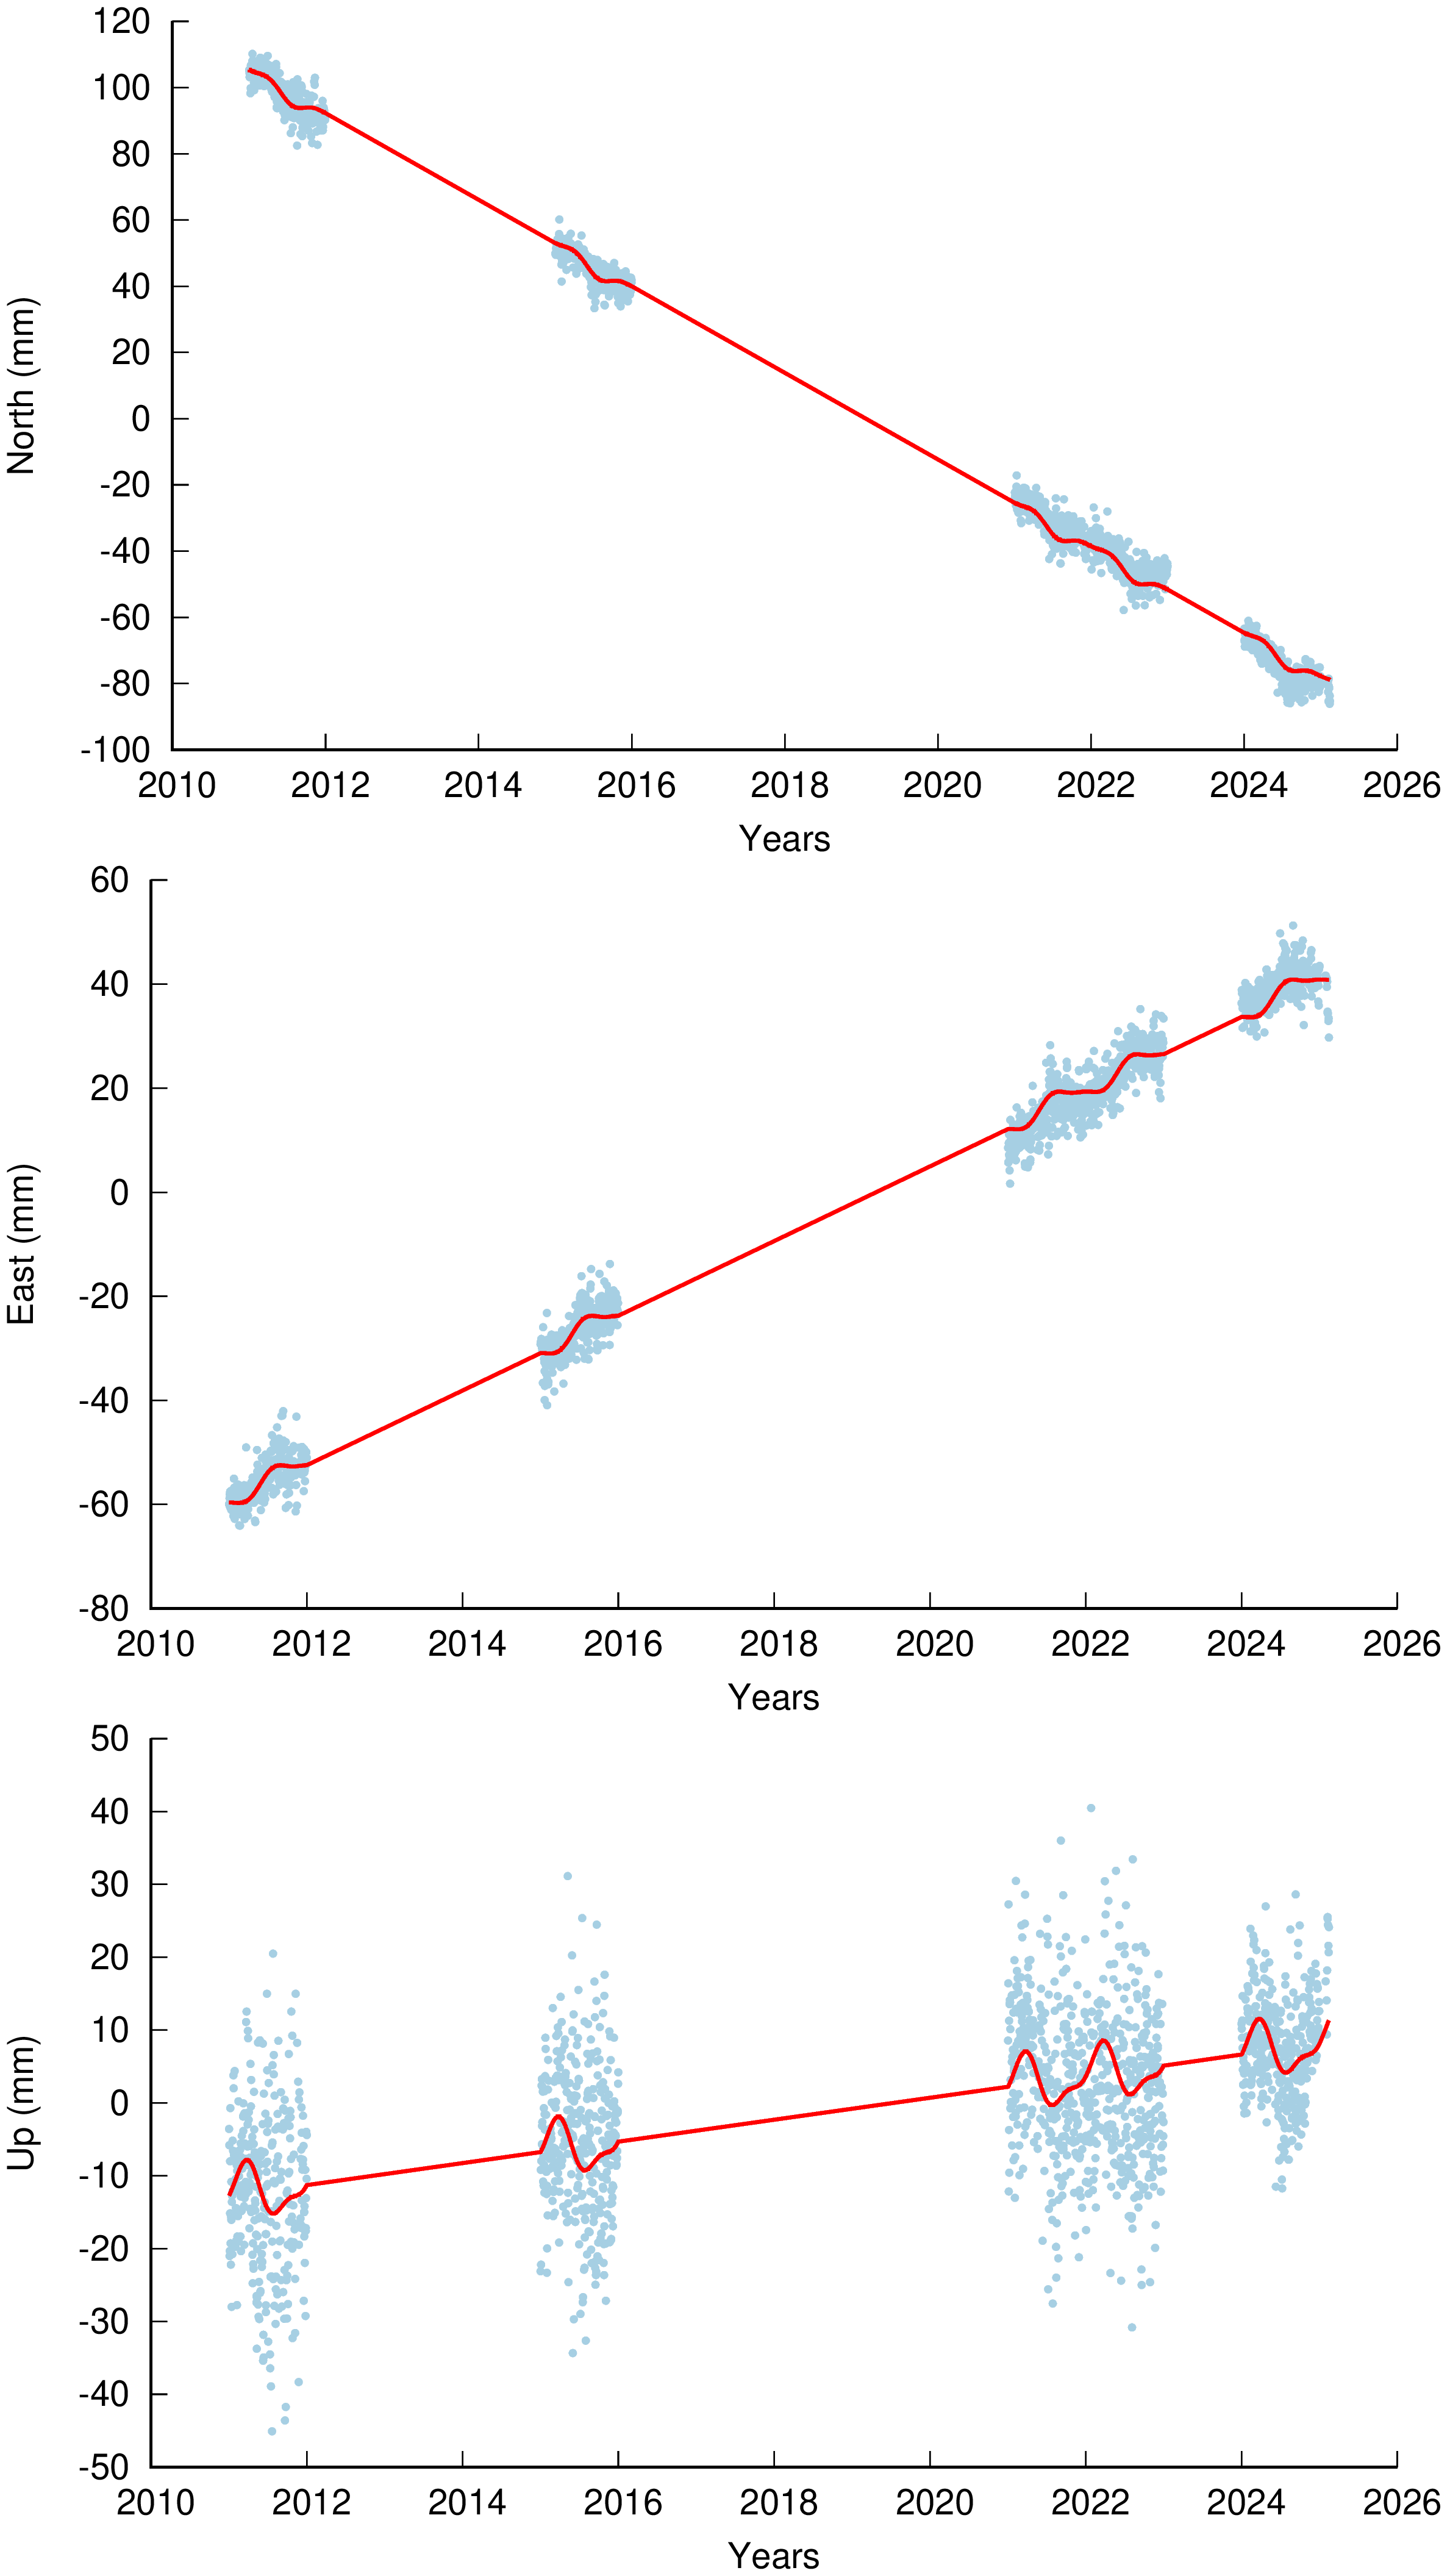
\includegraphics[width=.97\textwidth]{047a-mod.png}
      \end{center}  
    \end{column}
    \begin{column}{.25\textwidth}
      \begin{center}
       {\scriptsize 049A (Ίος)}
        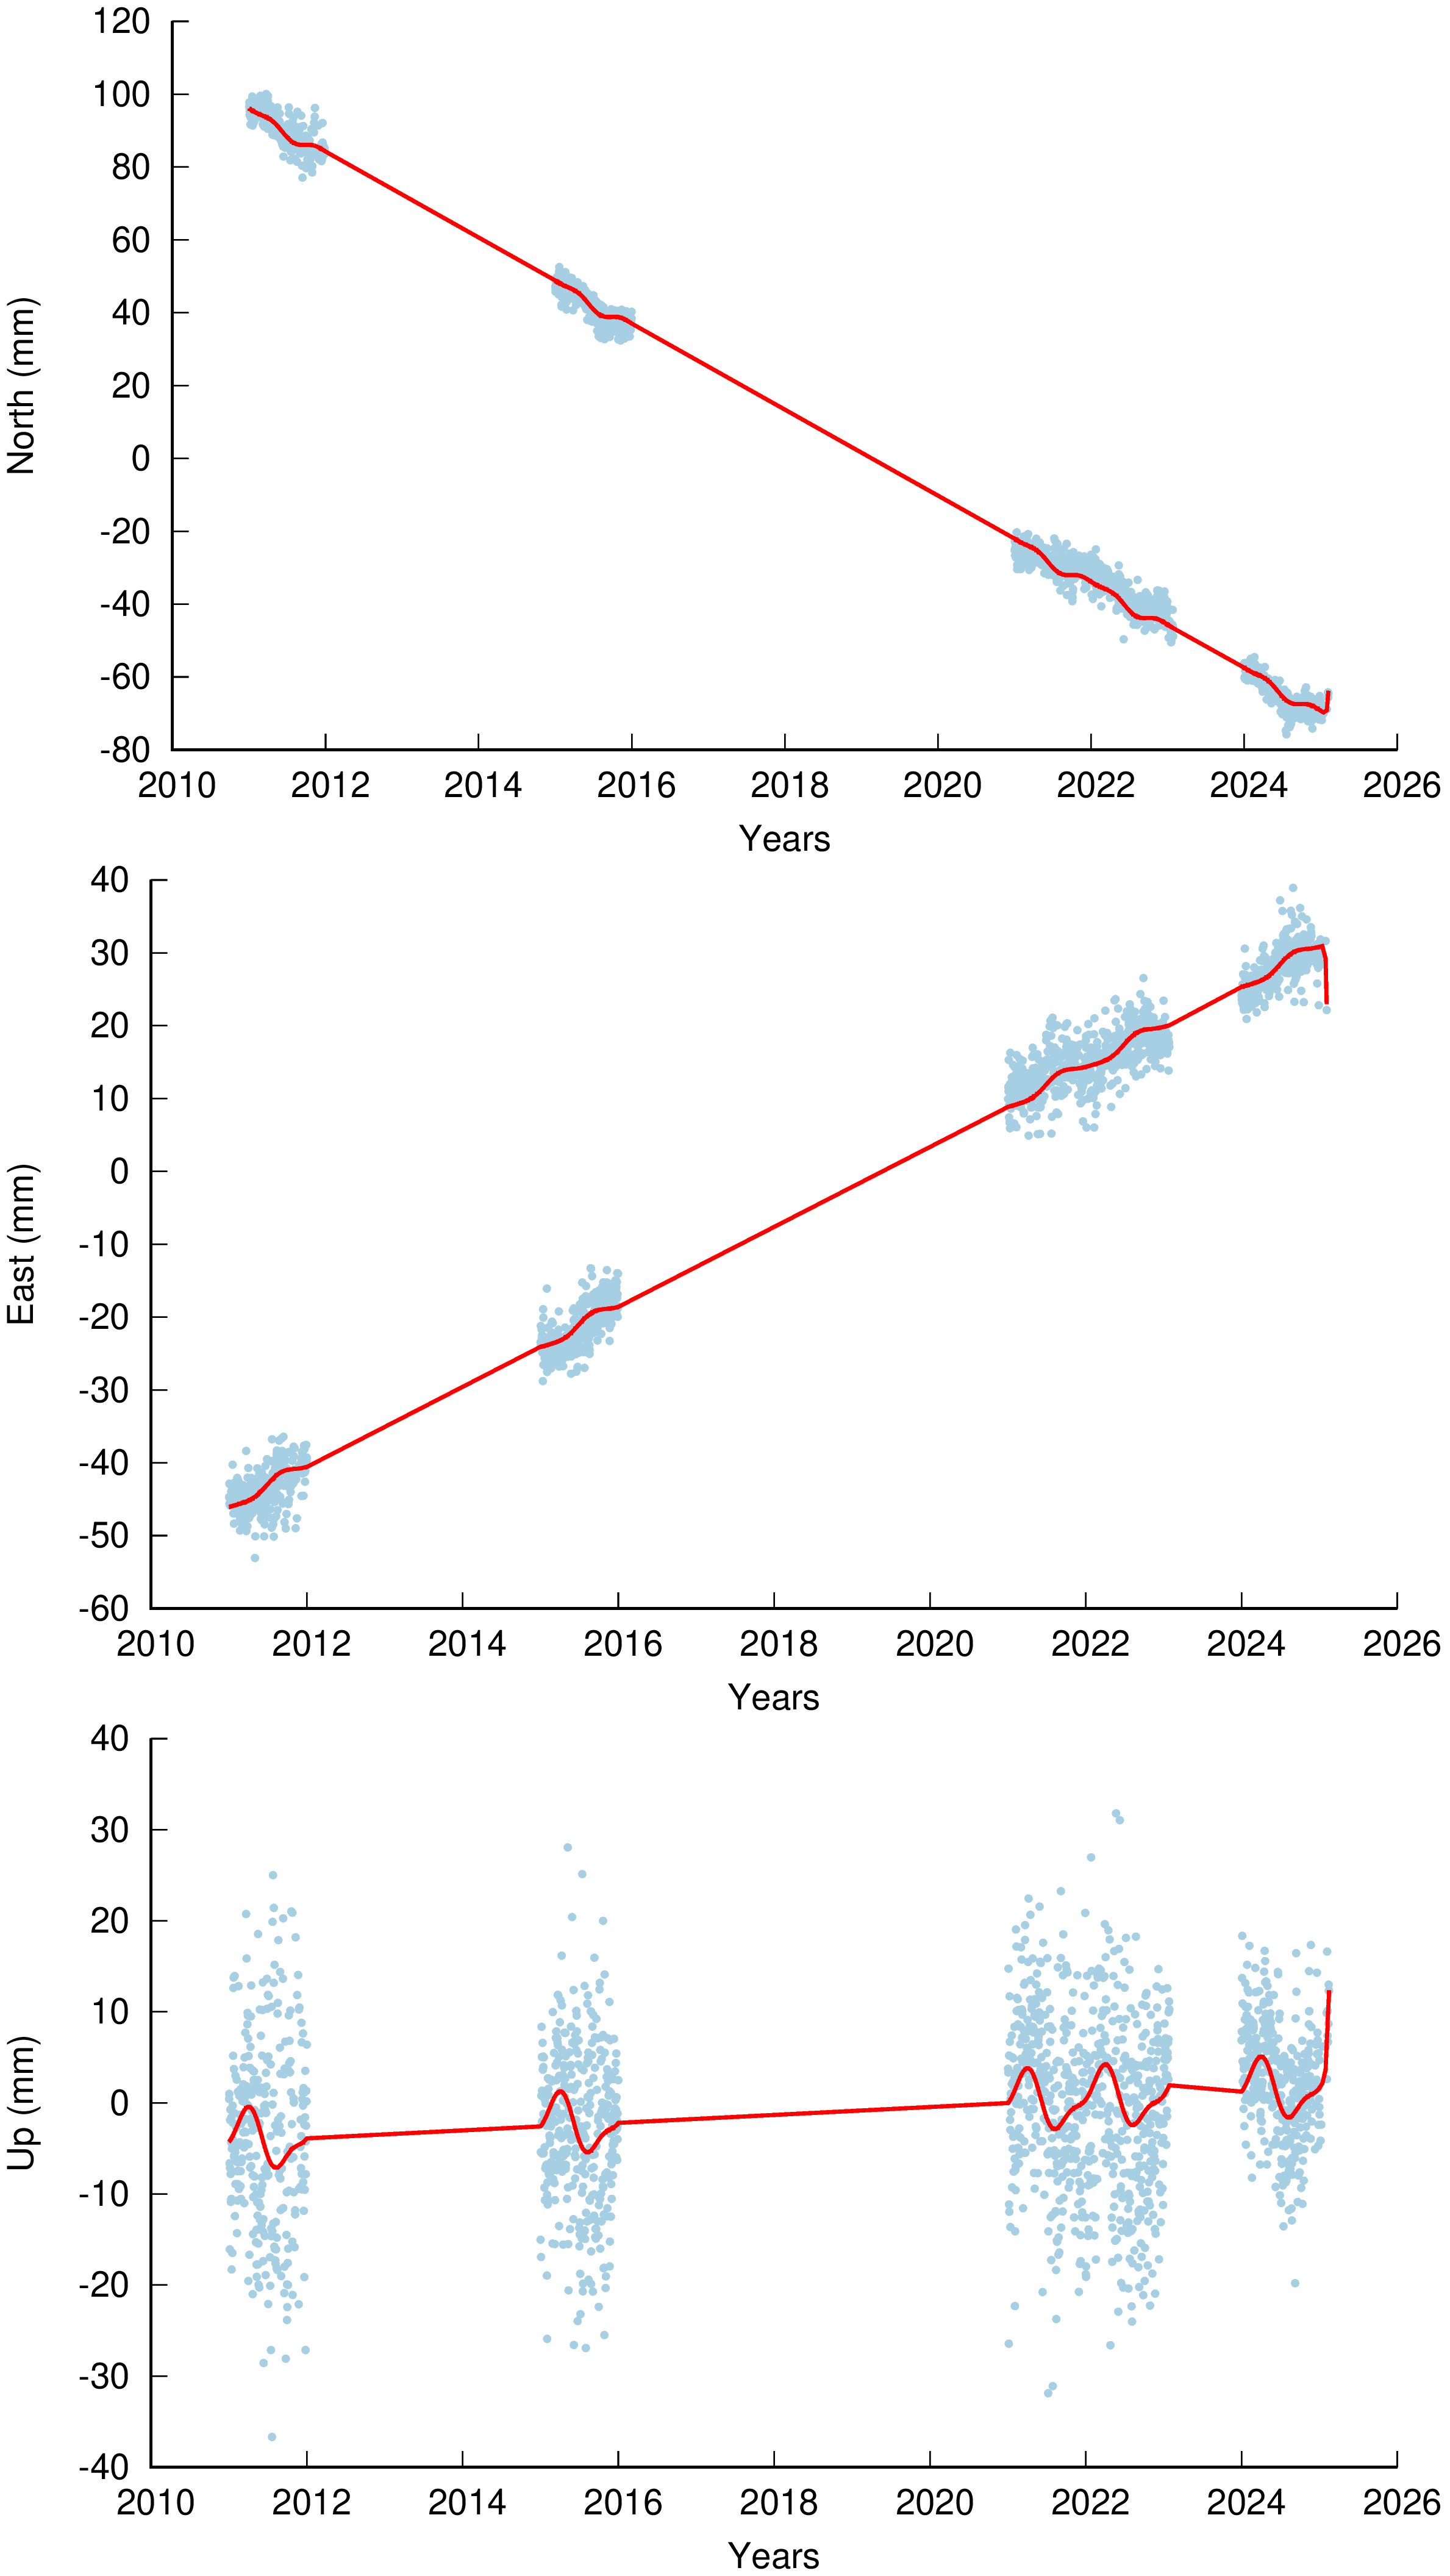
\includegraphics[width=.97\textwidth]{049a-mod.png}
      \end{center}       
    \end{column}
  \begin{column}{.25\textwidth}
      \begin{center}
       {\scriptsize 048A (Θήρα)}
        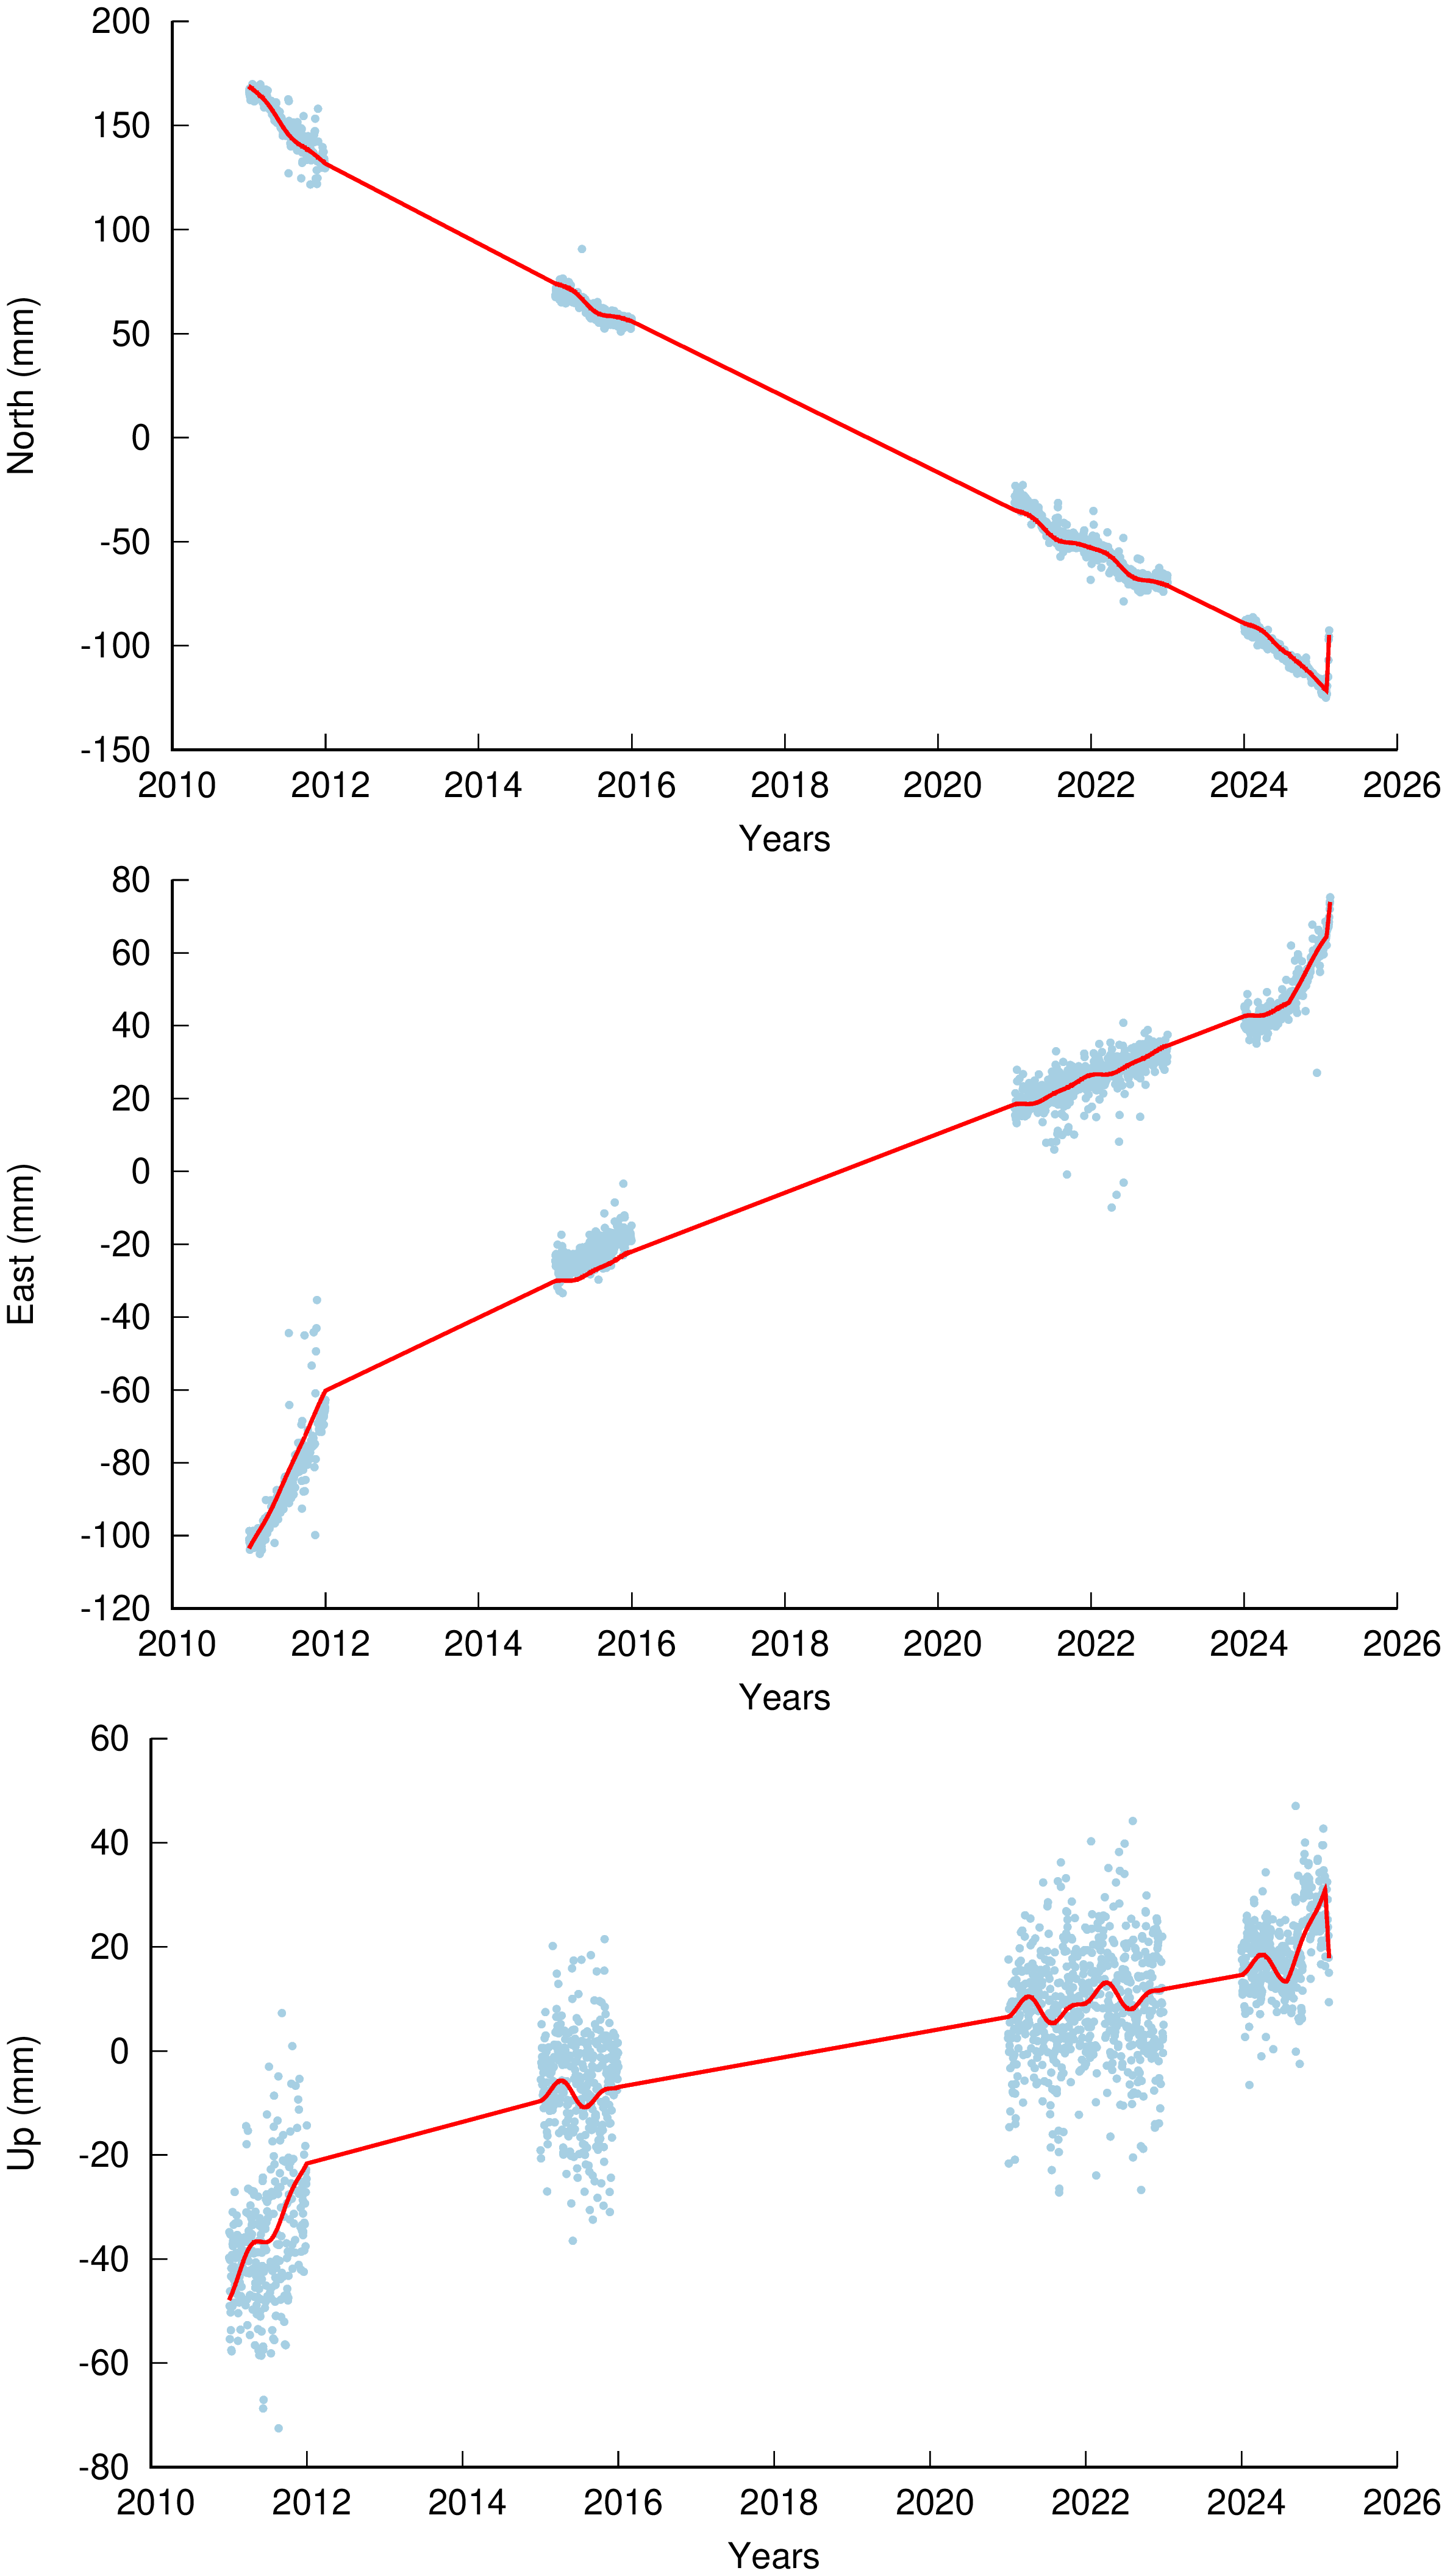
\includegraphics[width=.97\textwidth]{048a-mod.png}
      \end{center}  
    \end{column}
    \begin{column}{.25\textwidth}
      \begin{center}
       {\scriptsize SNTR (Φάρος)}
        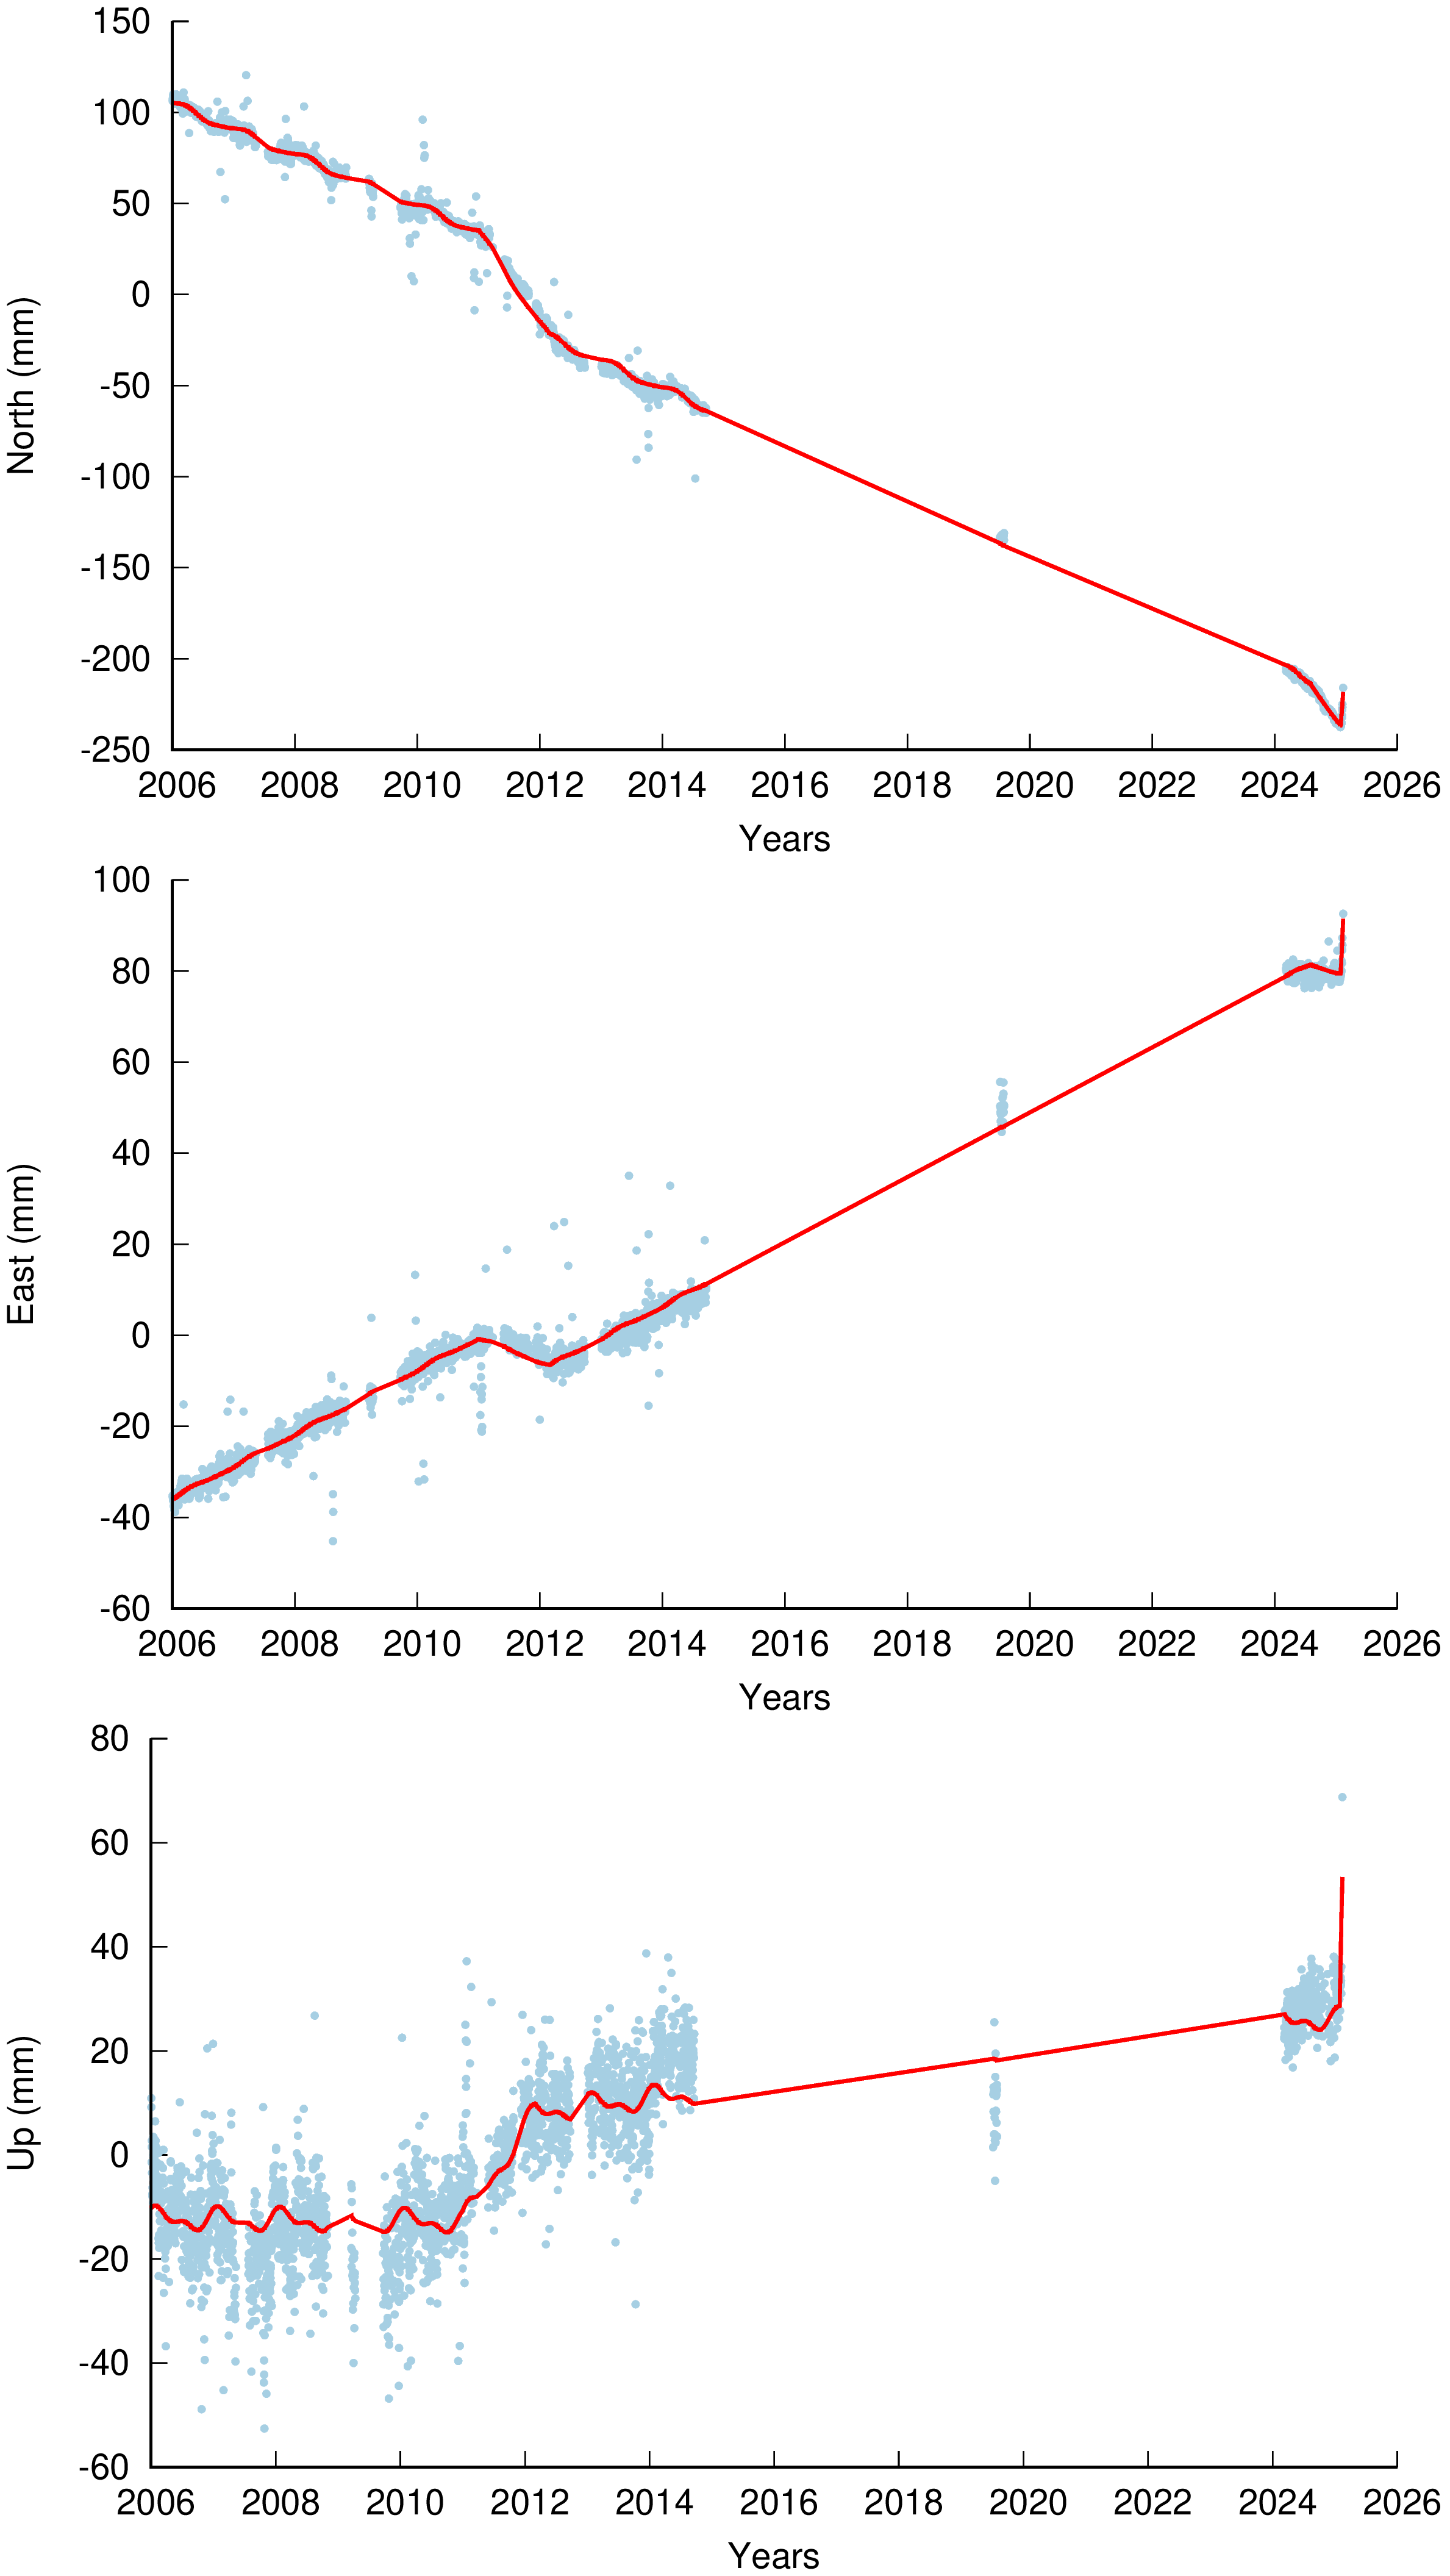
\includegraphics[width=.97\textwidth]{sntr-mod.png}
      \end{center}       
    \end{column}
  \end{columns}  
  
\end{frame}
\note{}

 % ------------------------------------------------------------------------------
\begin{frame}
  \frametitle{Μετακινήσεις 2024.6 - 2025.1 }
  \framesubtitle{}
  \label{}
  \vskip-.5cm
  \begin{columns}[T]
    \begin{column}{.5\textwidth}
      \begin{center}
        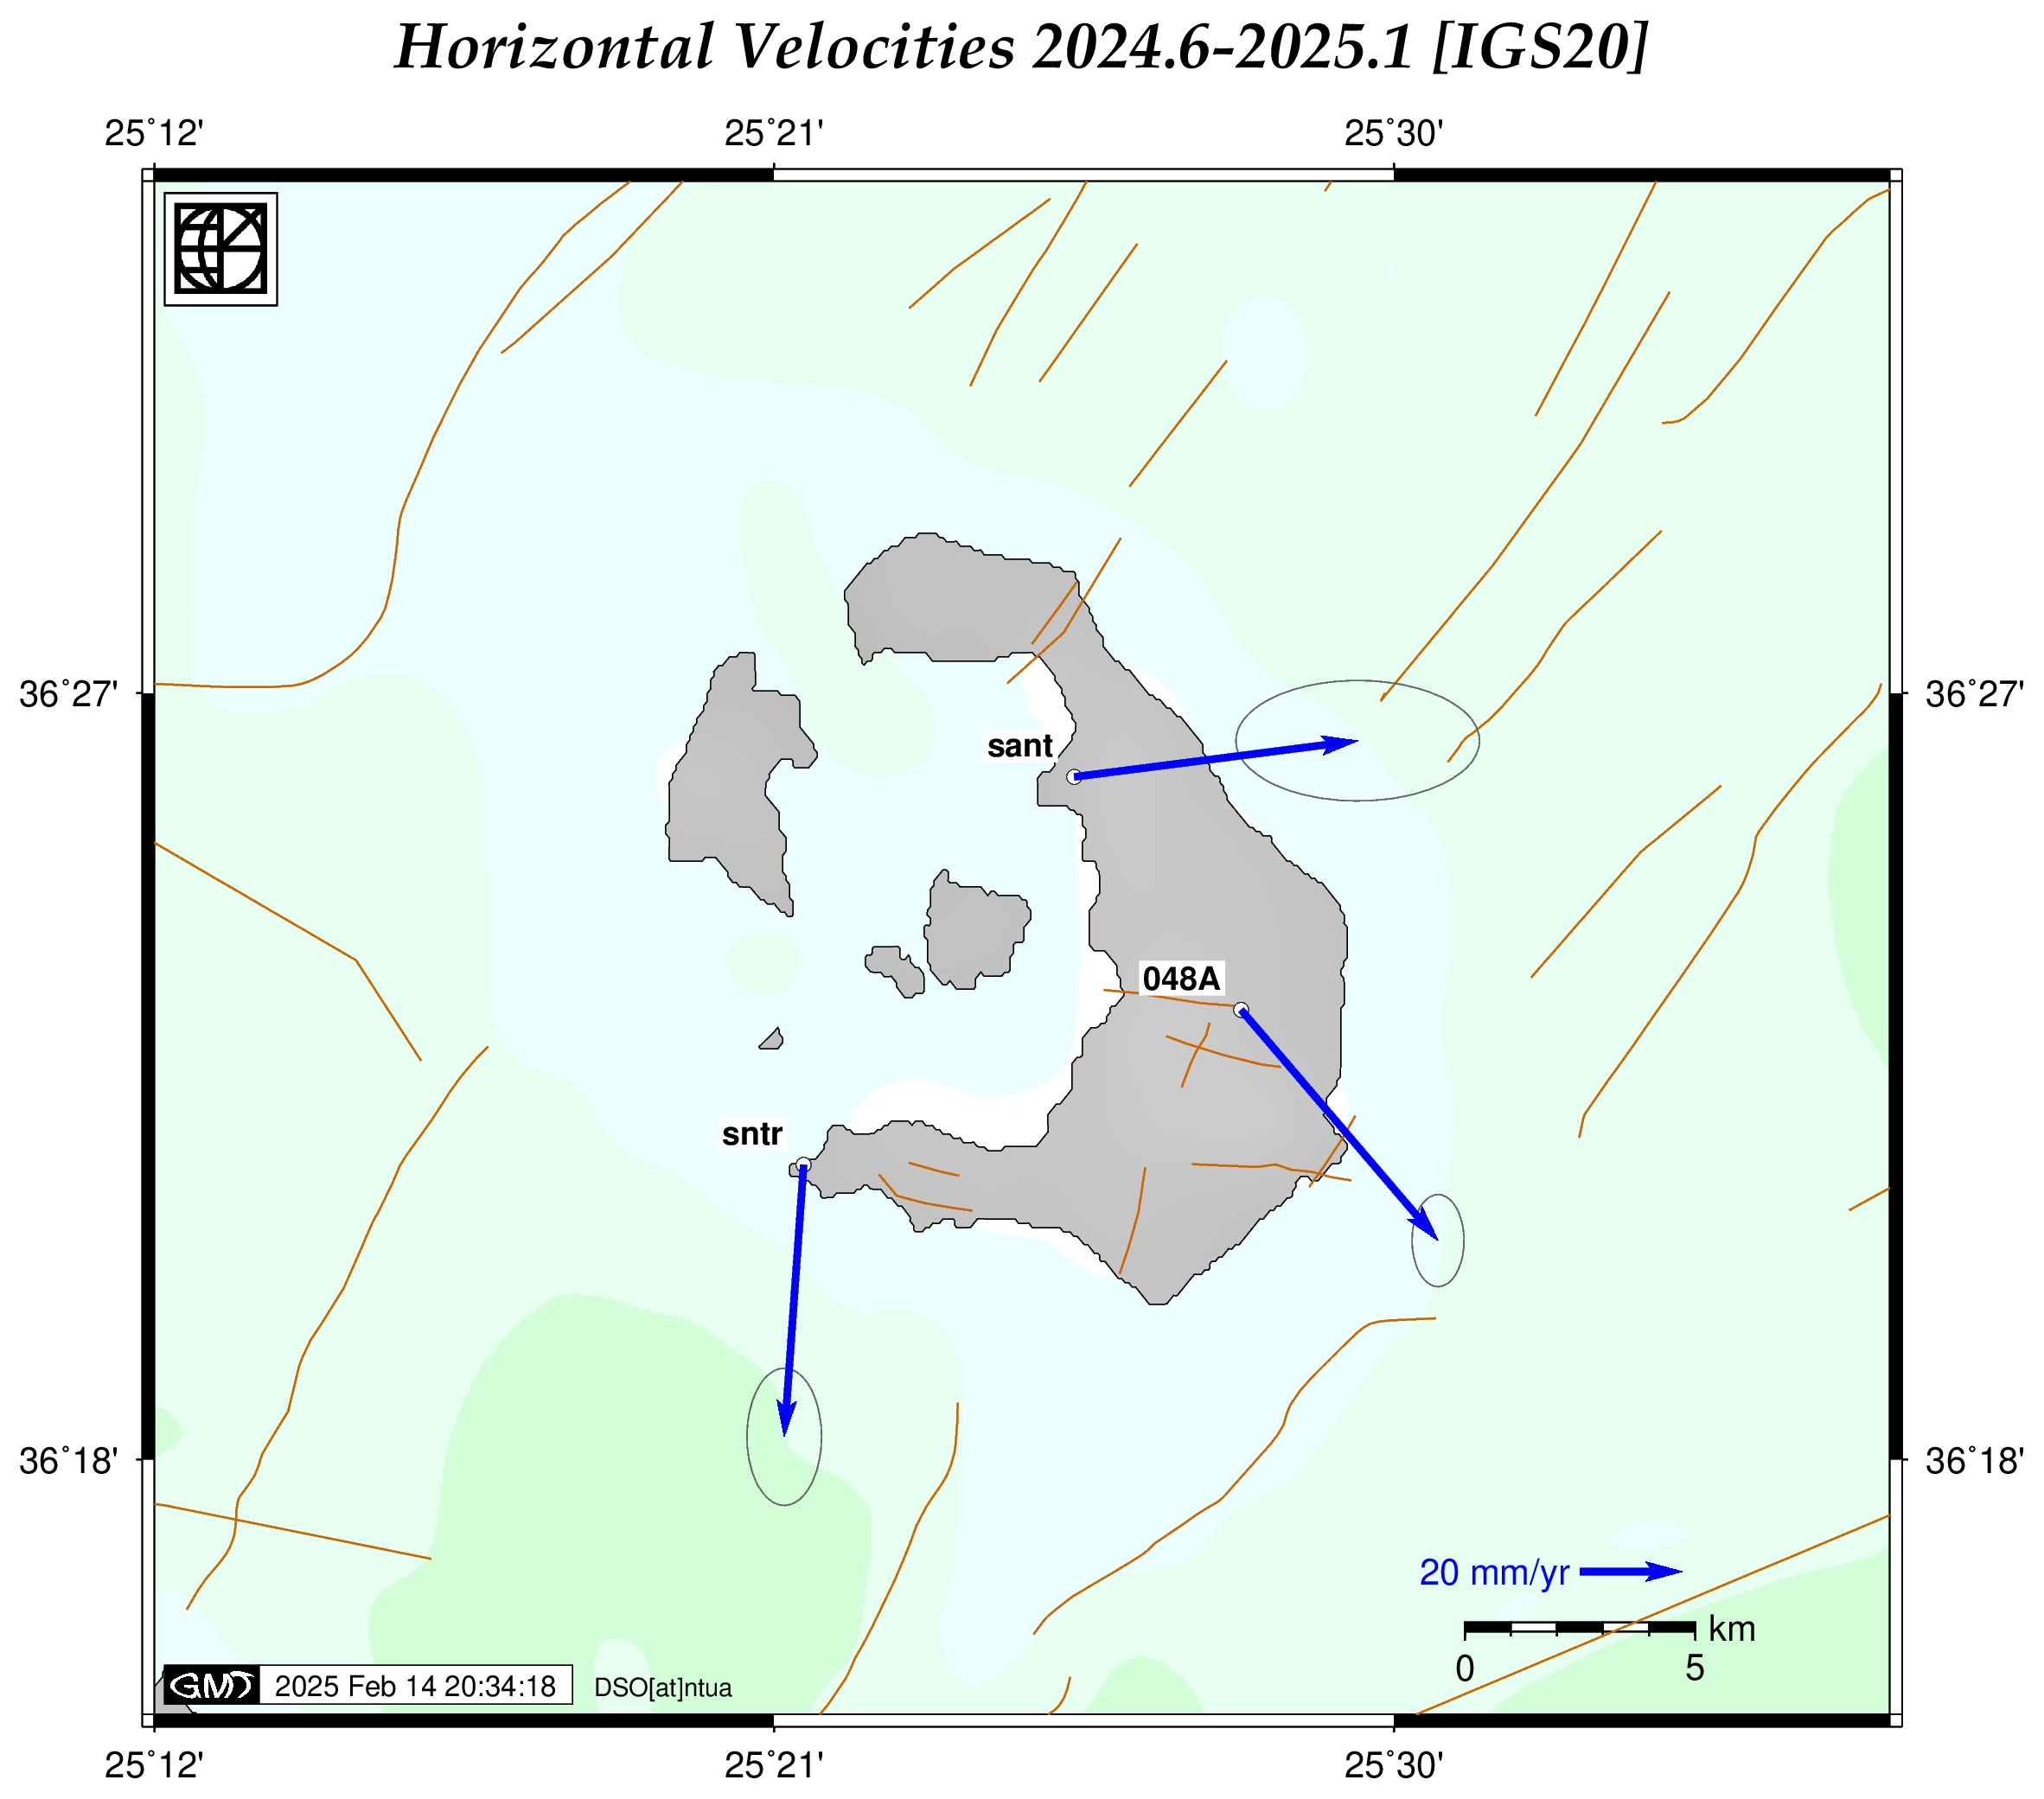
\includegraphics[width=.97\textwidth]{sant_2425_vhor.jpg}
      \end{center}  
    \end{column}
    \begin{column}{.5\textwidth}
      \begin{center}
        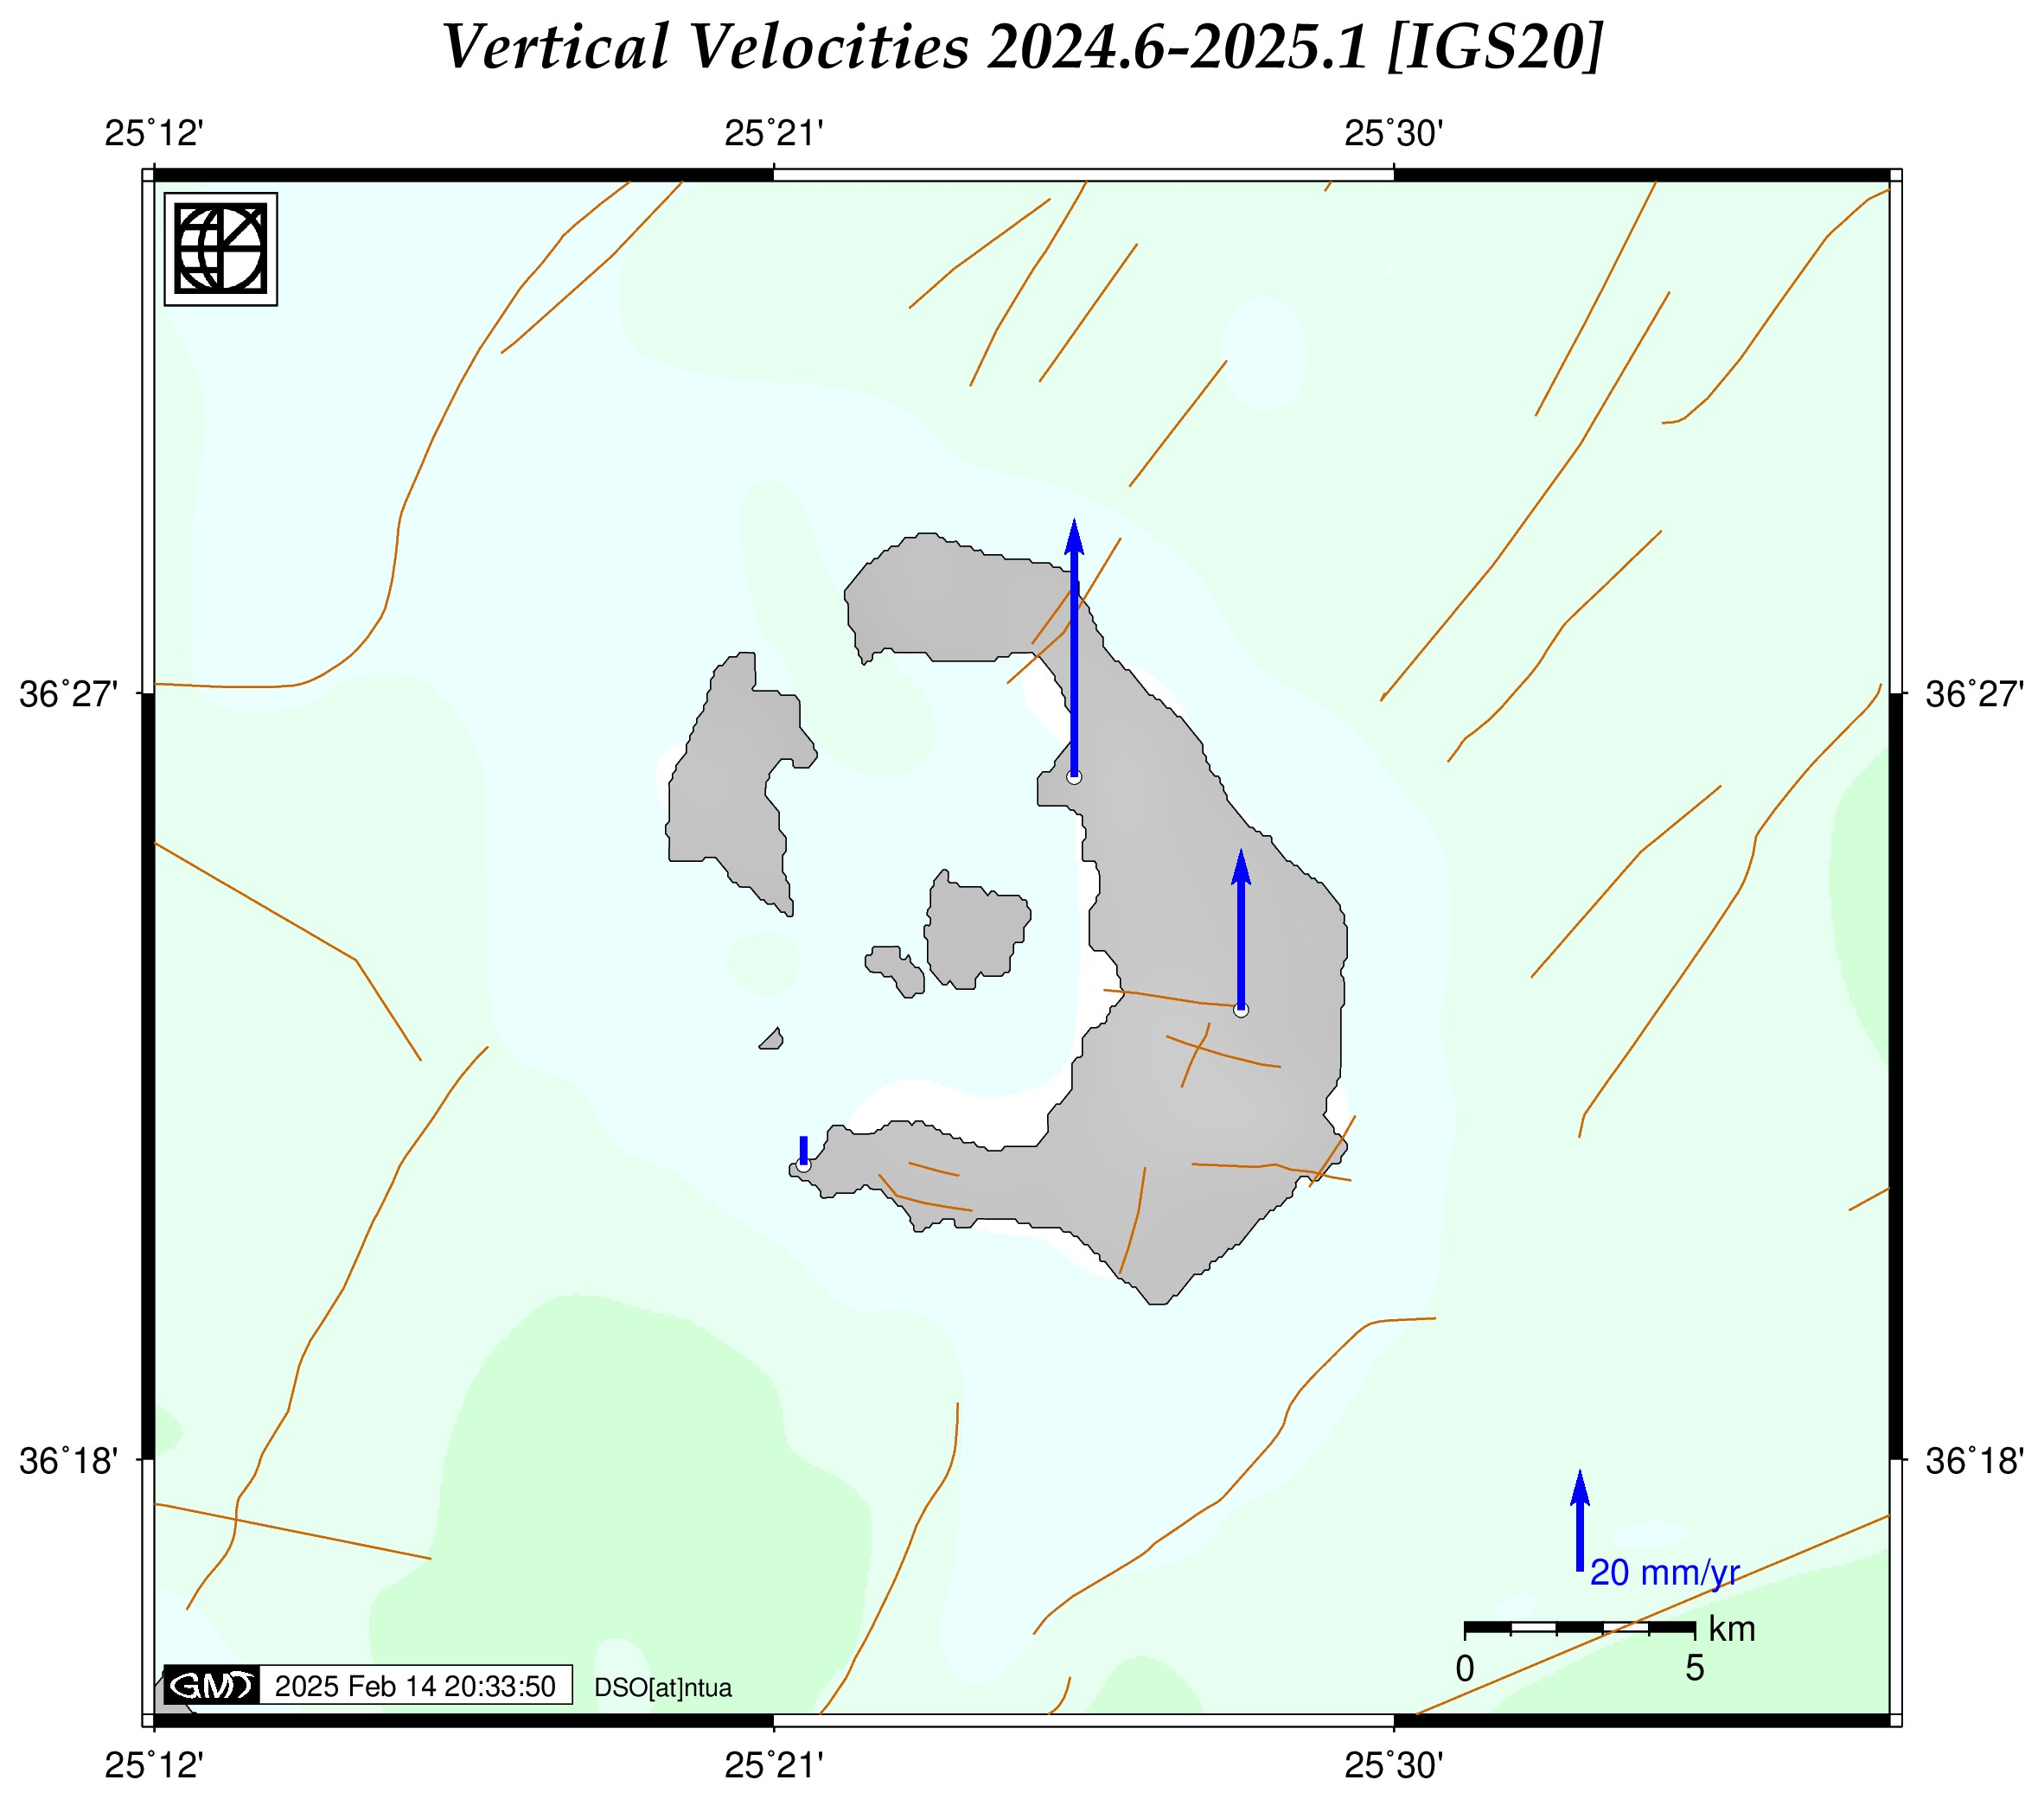
\includegraphics[width=.97\textwidth]{sant_2425_vver.jpg}
      \end{center}       
    \end{column}
  \end{columns}  

\end{frame}
\note{}



 % ------------------------------------------------------------------------------
\begin{frame}
  \frametitle{Ανάλυση χρονοσειρών}
  \framesubtitle{}
  \label{}
  \vskip-1cm
  \begin{columns}[T]
    \begin{column}{.25\textwidth}
      \begin{center}
      {\scriptsize 047A (Αμοργός)}
        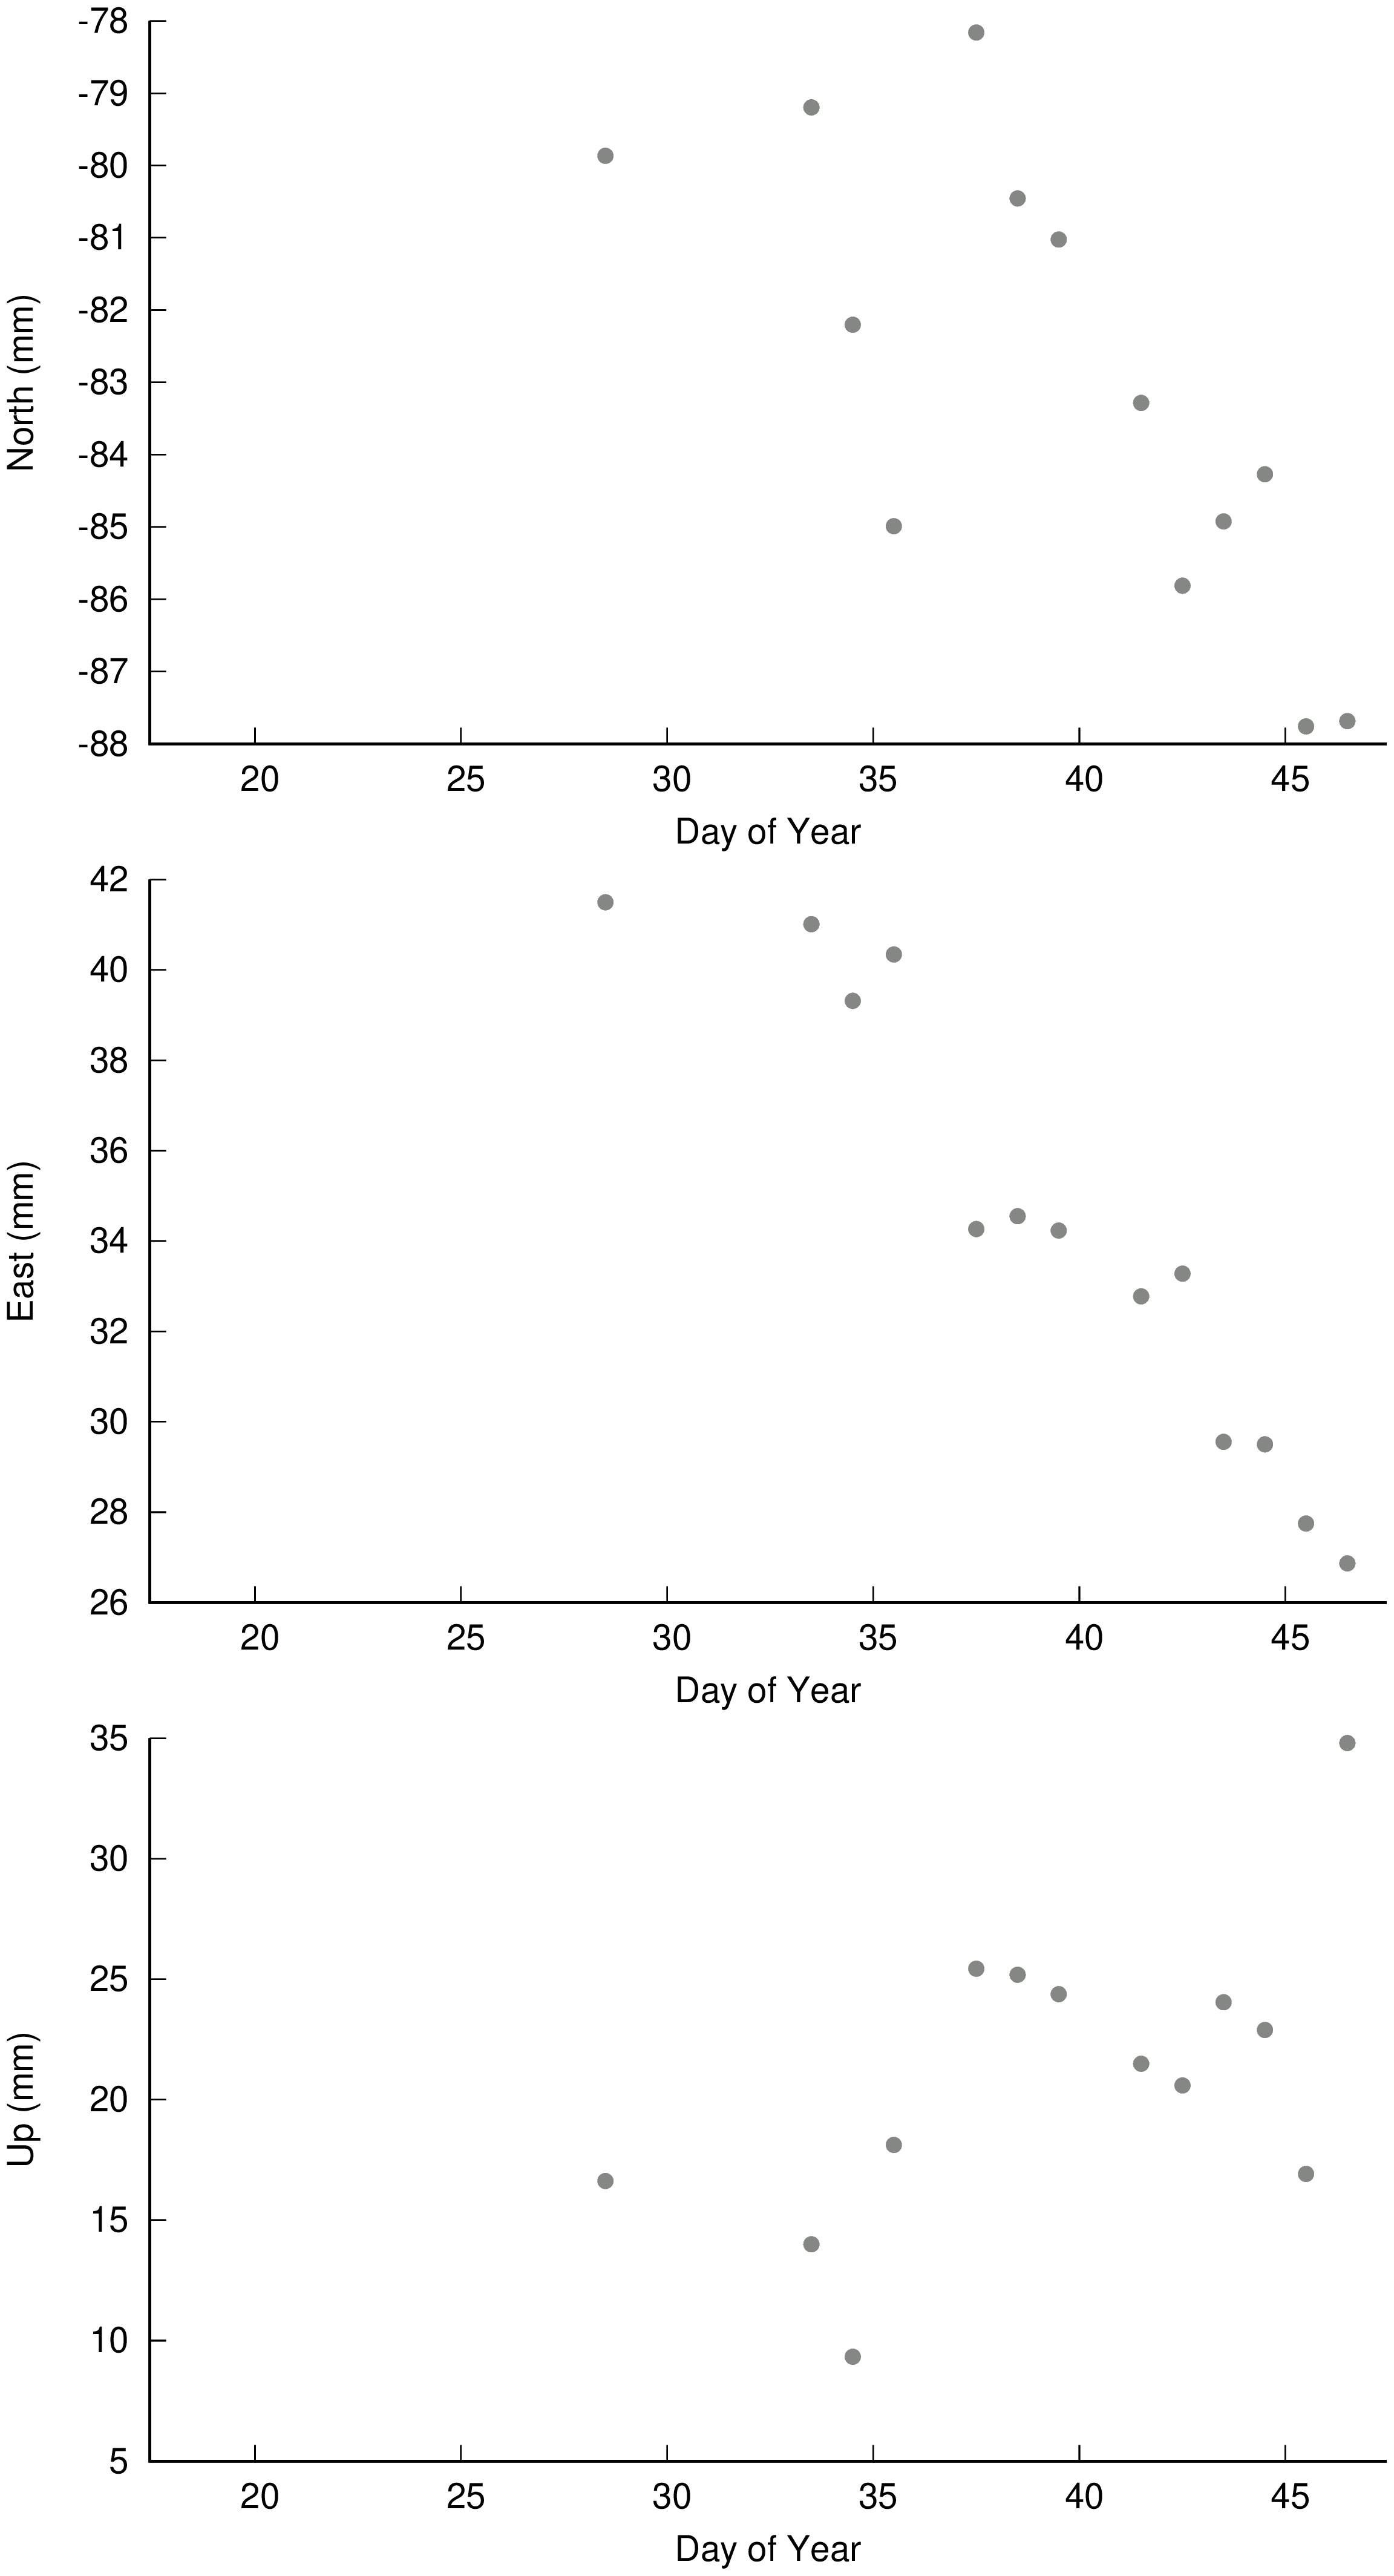
\includegraphics[width=.97\textwidth]{047a-lmn.png}
      \end{center}  
    \end{column}
    \begin{column}{.25\textwidth}
      \begin{center}
       {\scriptsize 049A (Ίος)}
        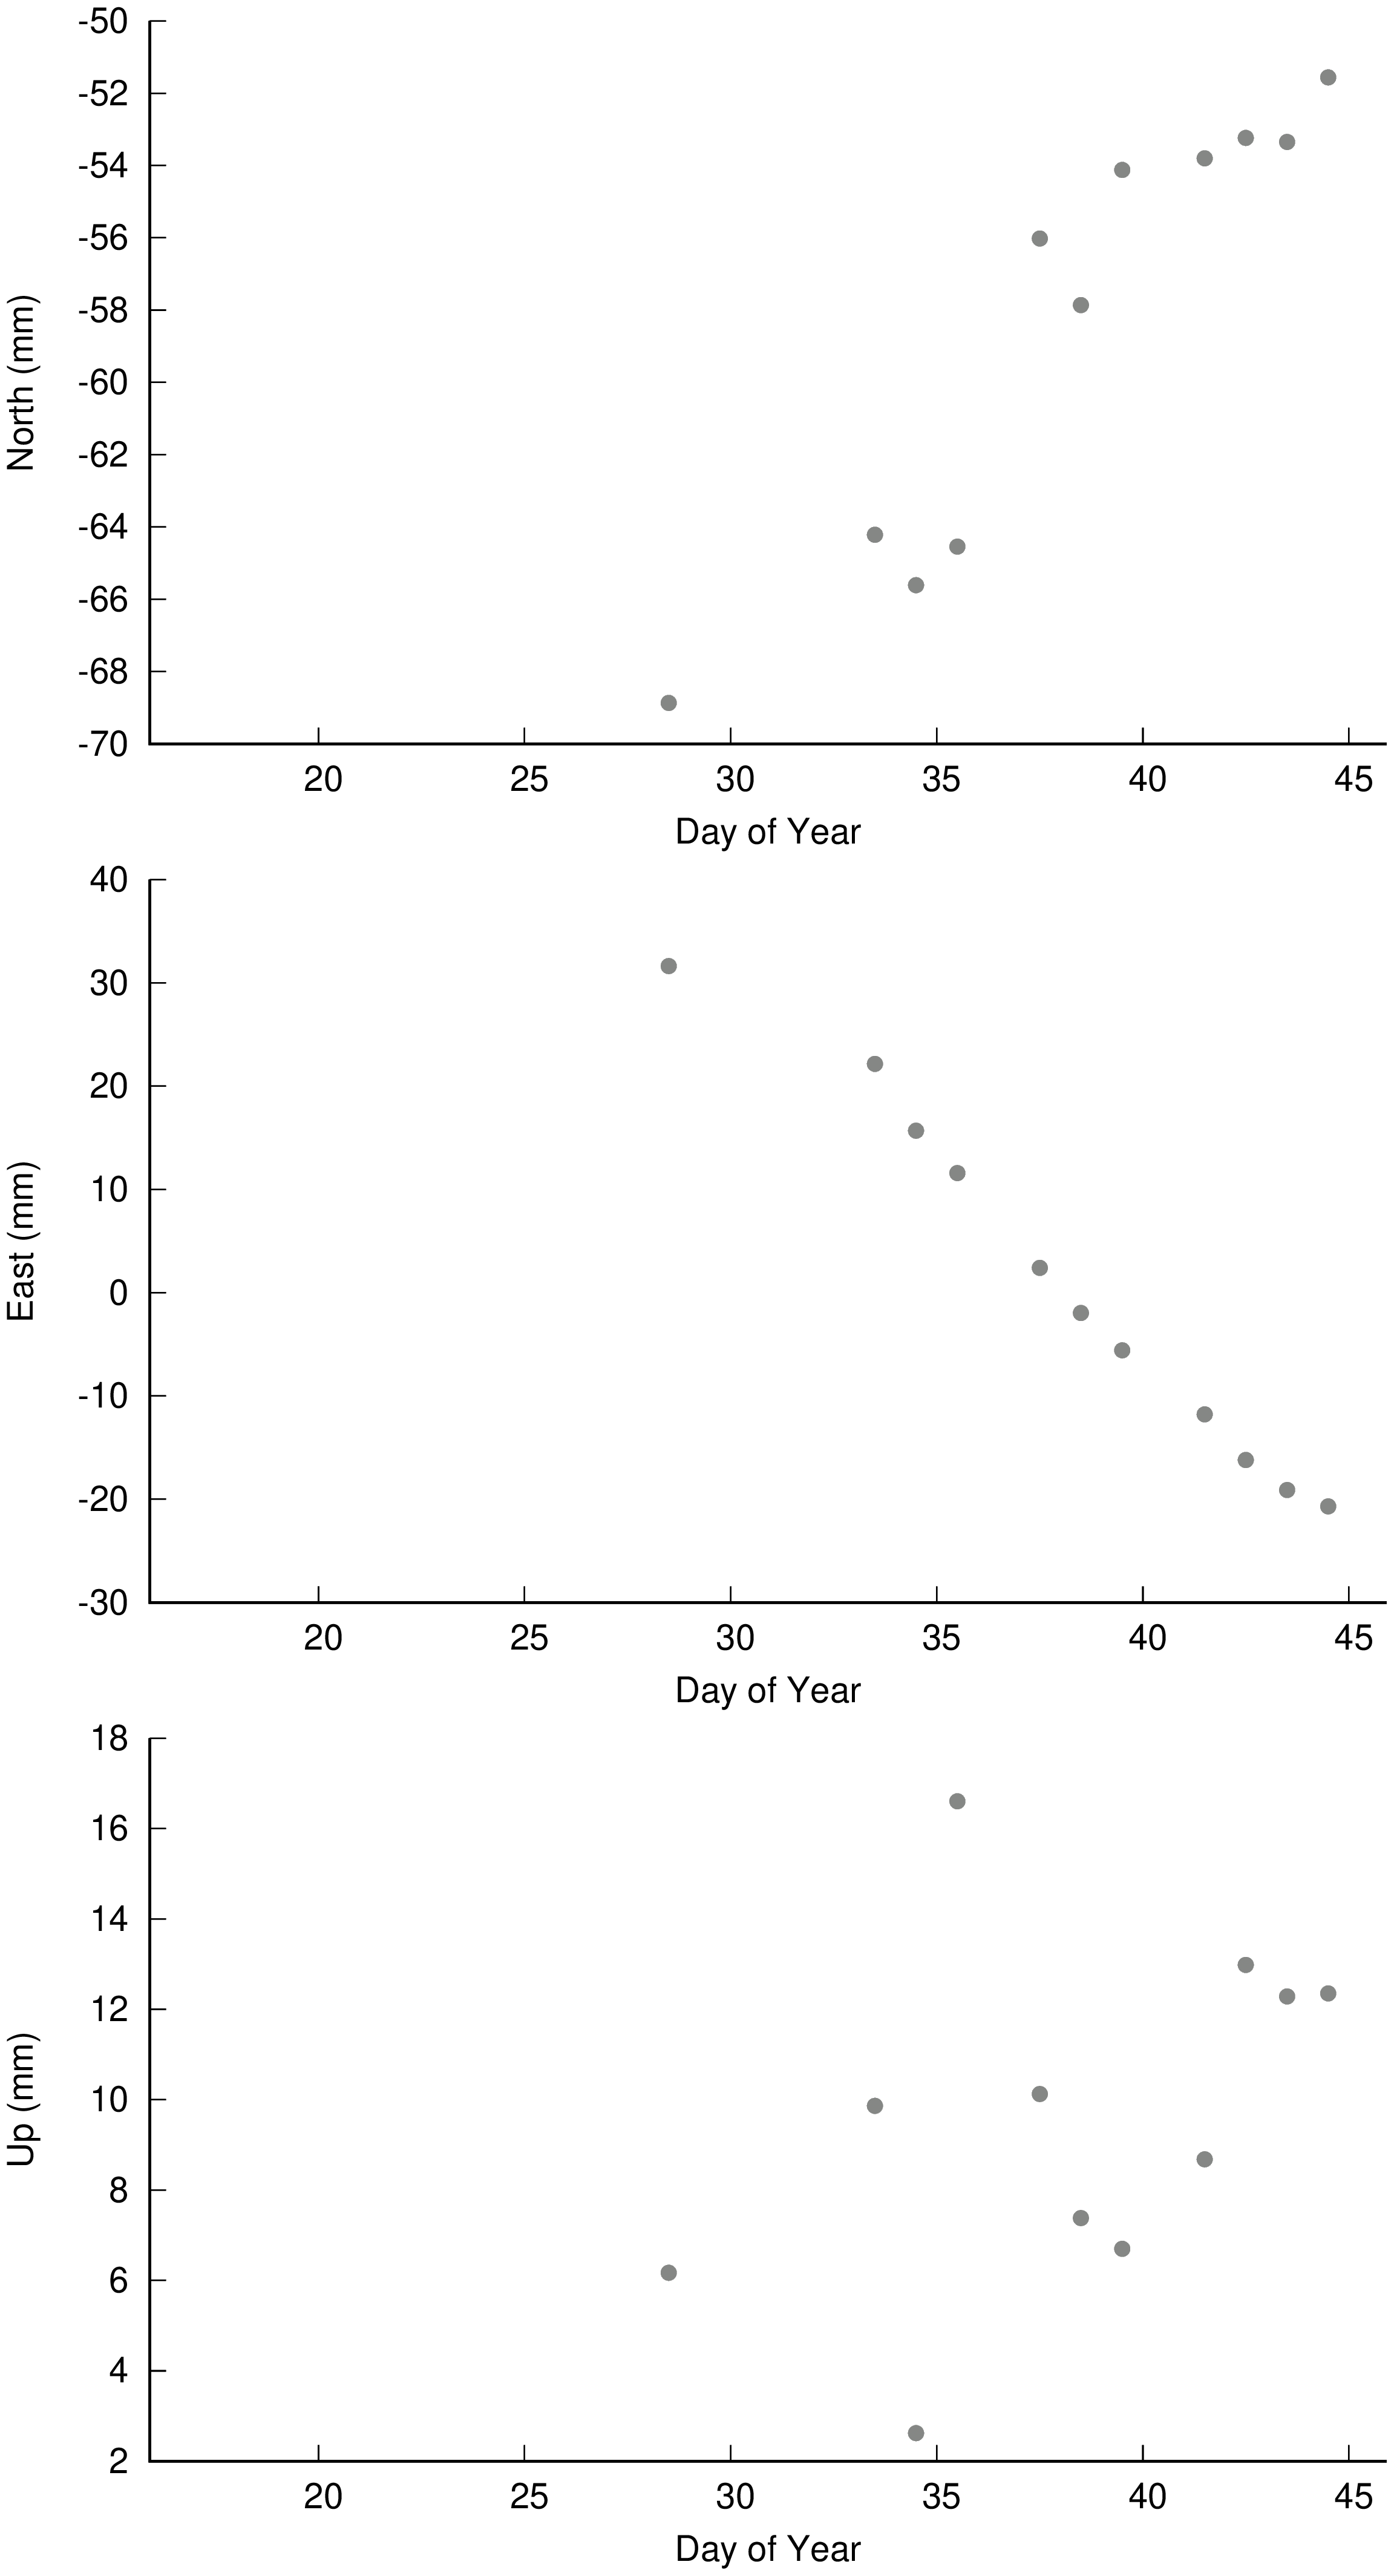
\includegraphics[width=.97\textwidth]{049a-lmn.png}
      \end{center}       
    \end{column}
  \begin{column}{.25\textwidth}
      \begin{center}
       {\scriptsize 048A (Θήρα)}
        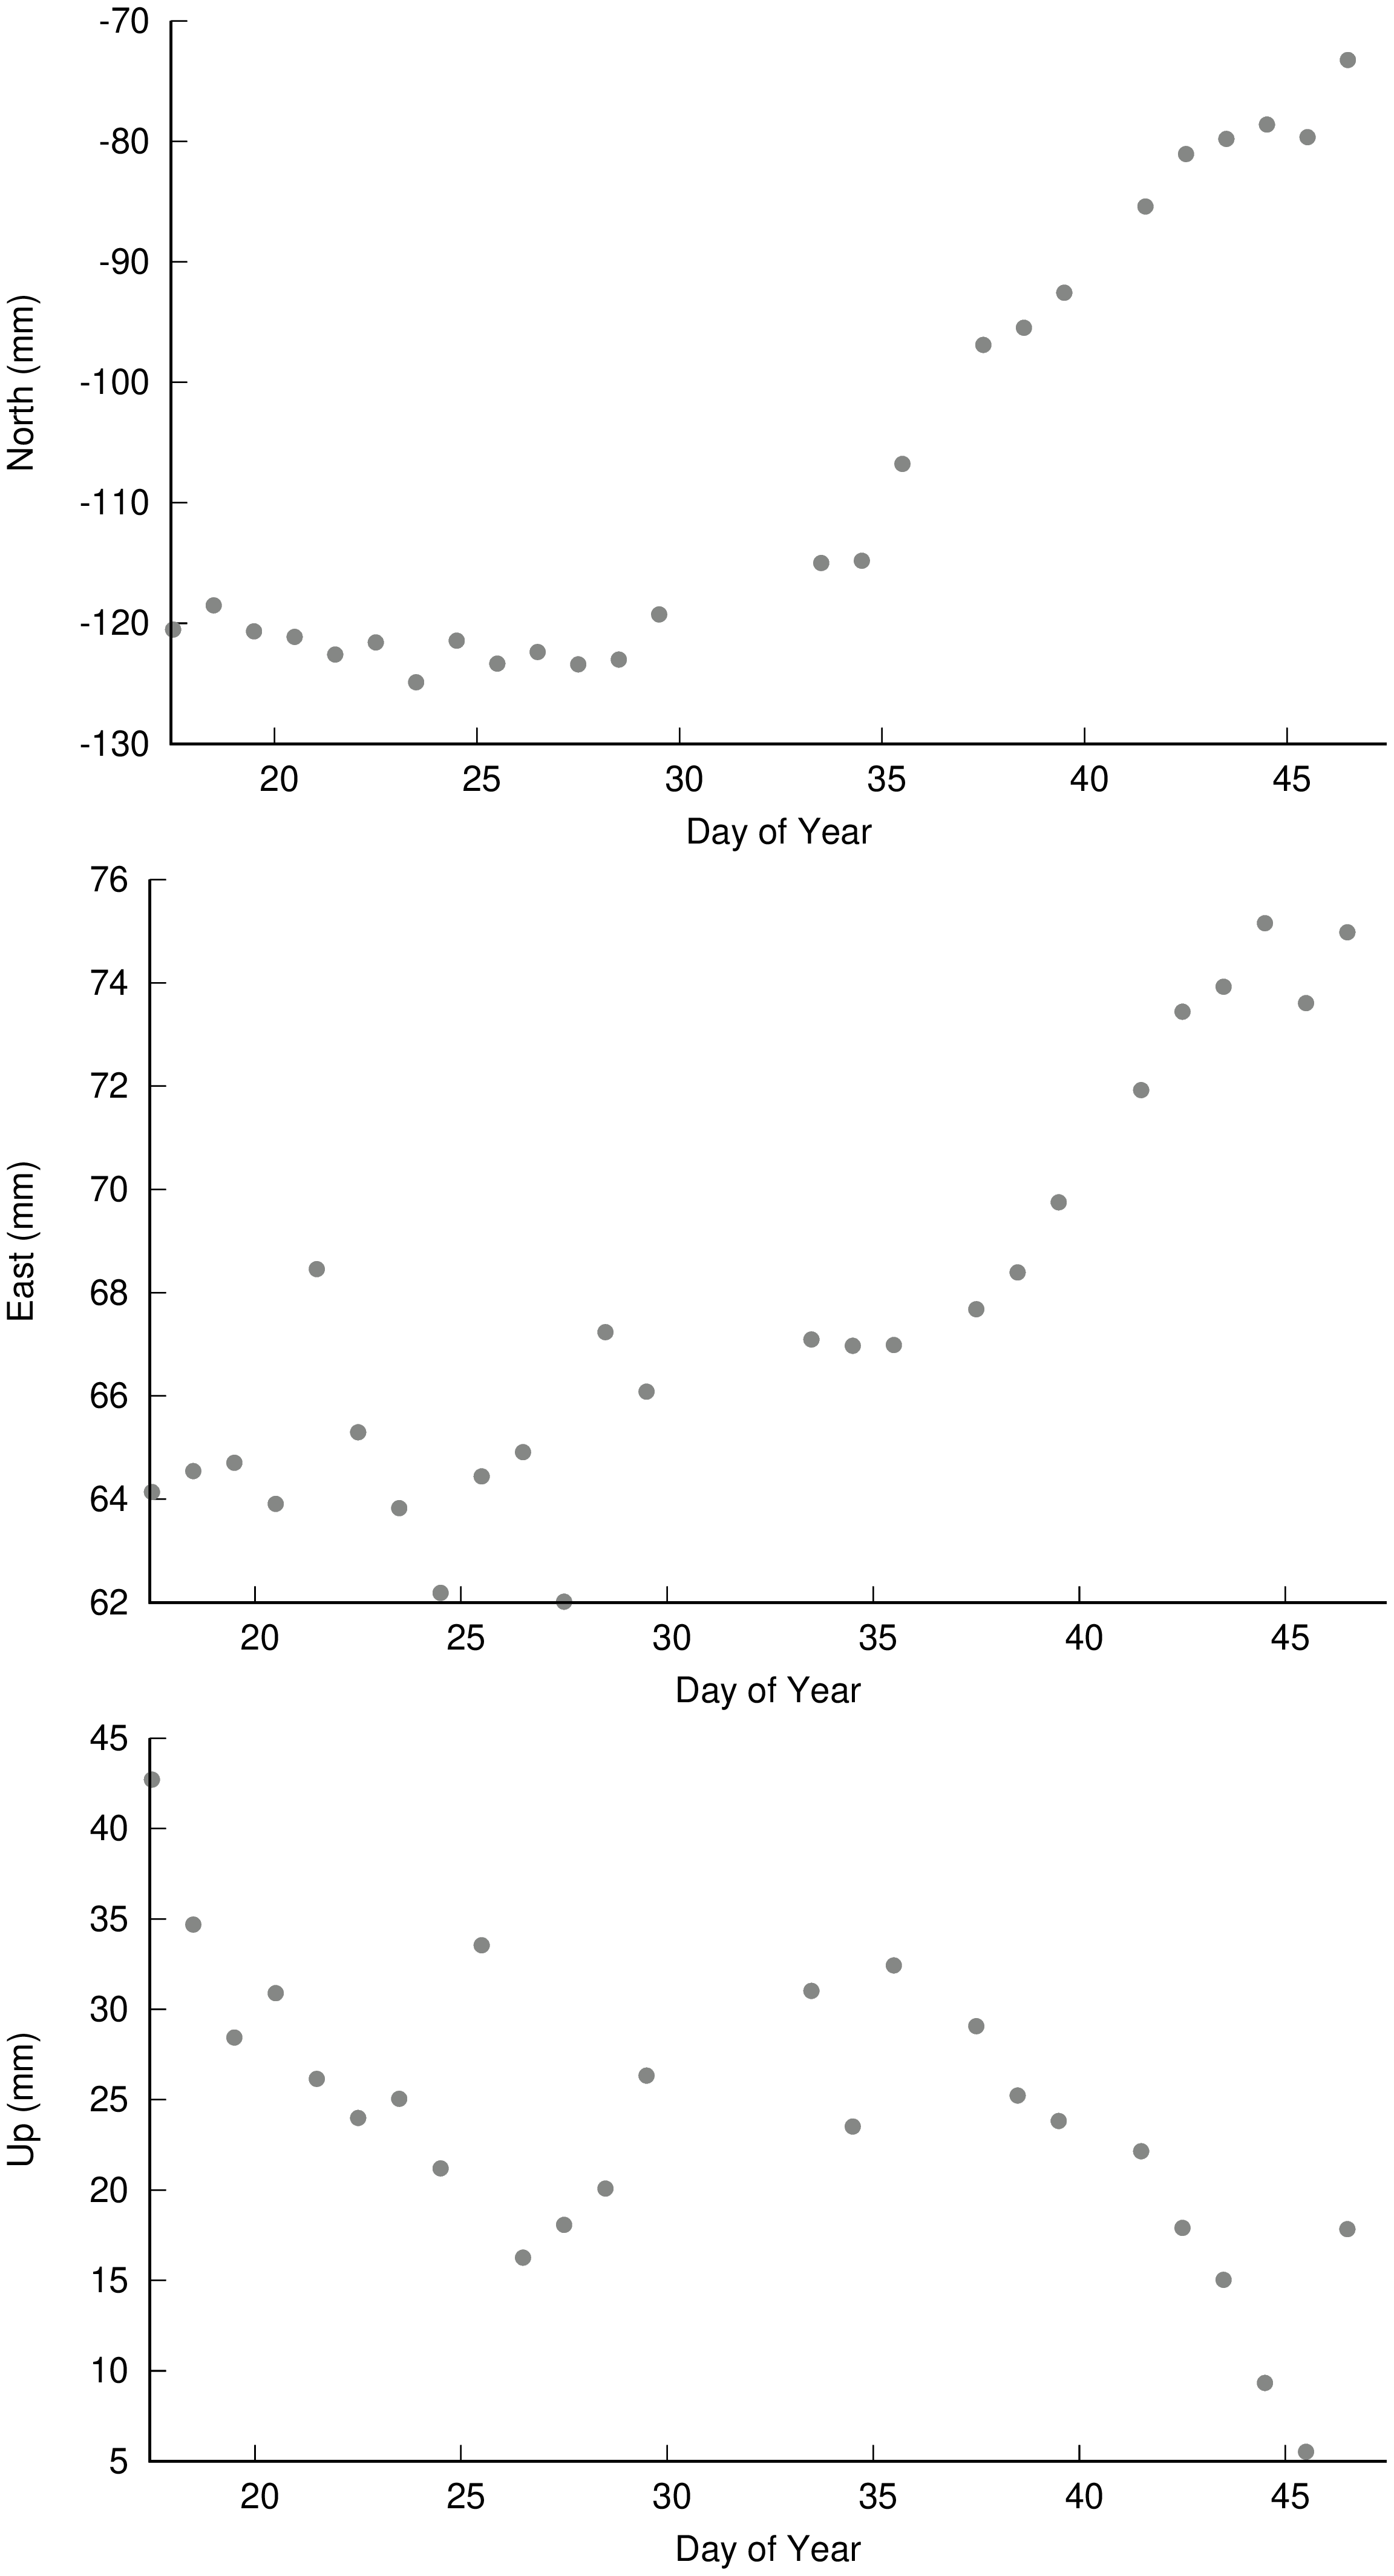
\includegraphics[width=.97\textwidth]{048a-lmn.png}
      \end{center}  
    \end{column}
    \begin{column}{.25\textwidth}
      \begin{center}
       {\scriptsize SNTR (Φάρος)}
        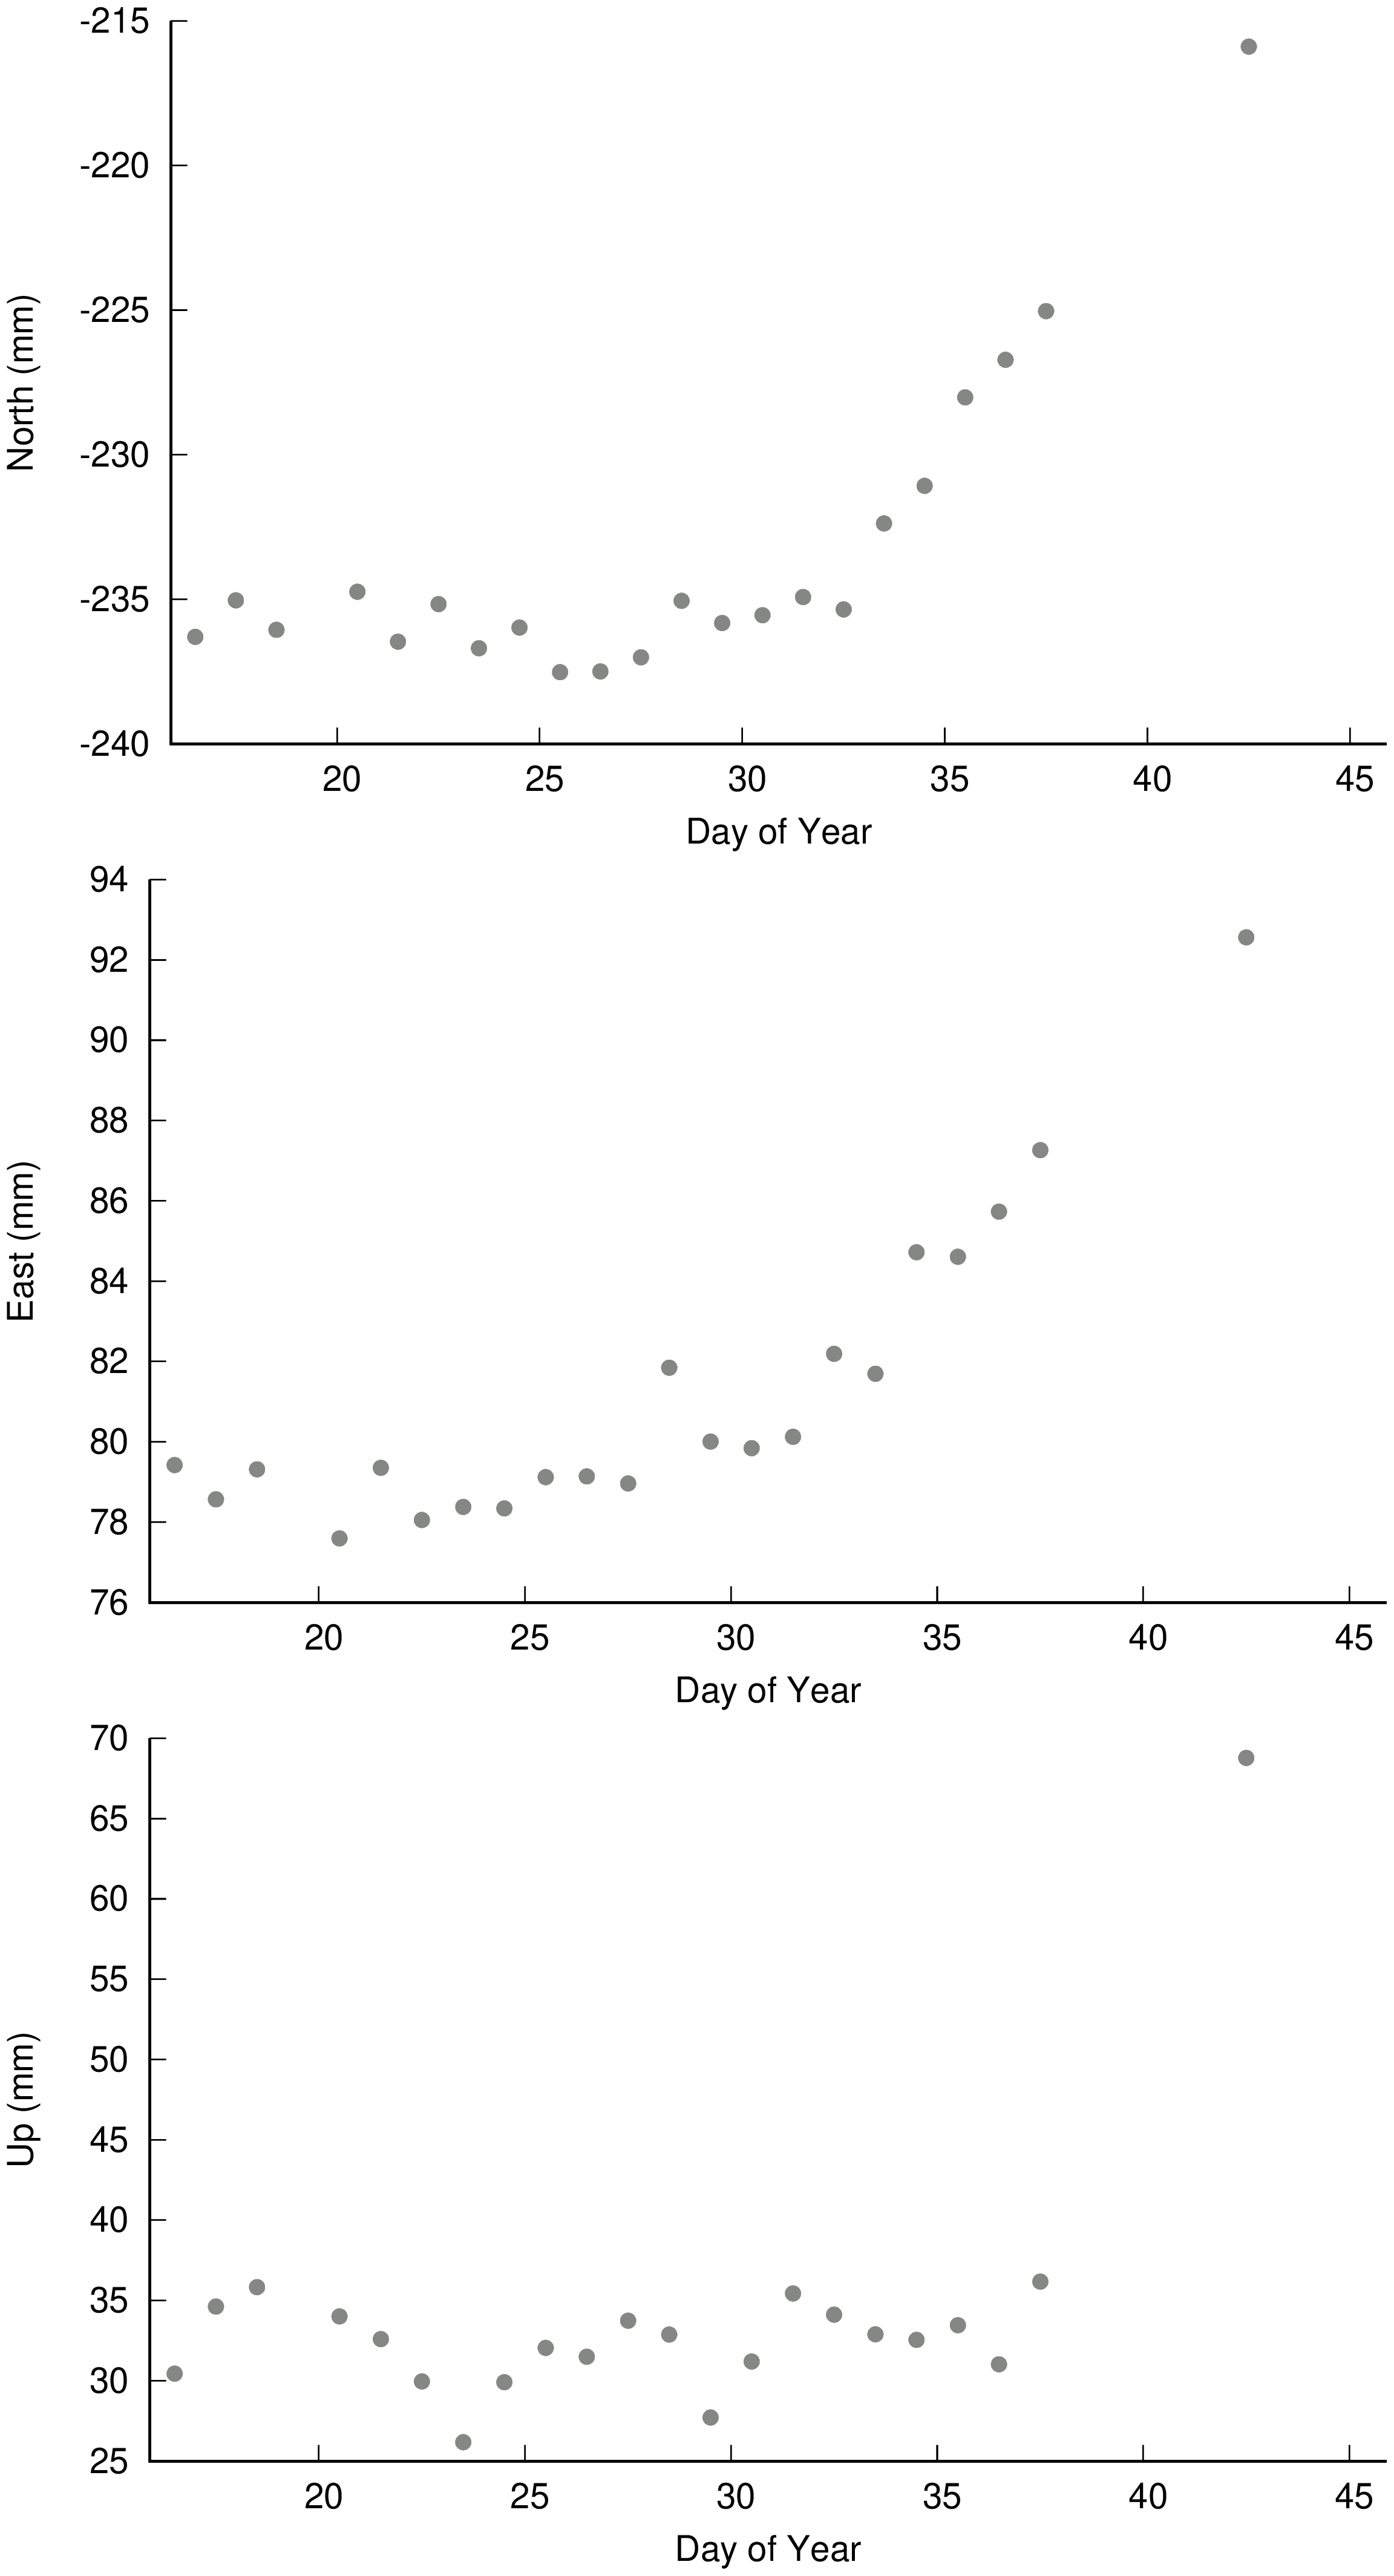
\includegraphics[width=.97\textwidth]{sntr-lmn.png}
      \end{center}       
    \end{column}
  \end{columns}  
  
\end{frame}
\note{}

 % ------------------------------------------------------------------------------
\begin{frame}
  \frametitle{Μετακινήσεις 2025 28/1 - 14/2 }
  \framesubtitle{}
  \label{}
  \vskip-.5cm
  \begin{columns}[T]
    \begin{column}{.5\textwidth}
      \begin{center}
        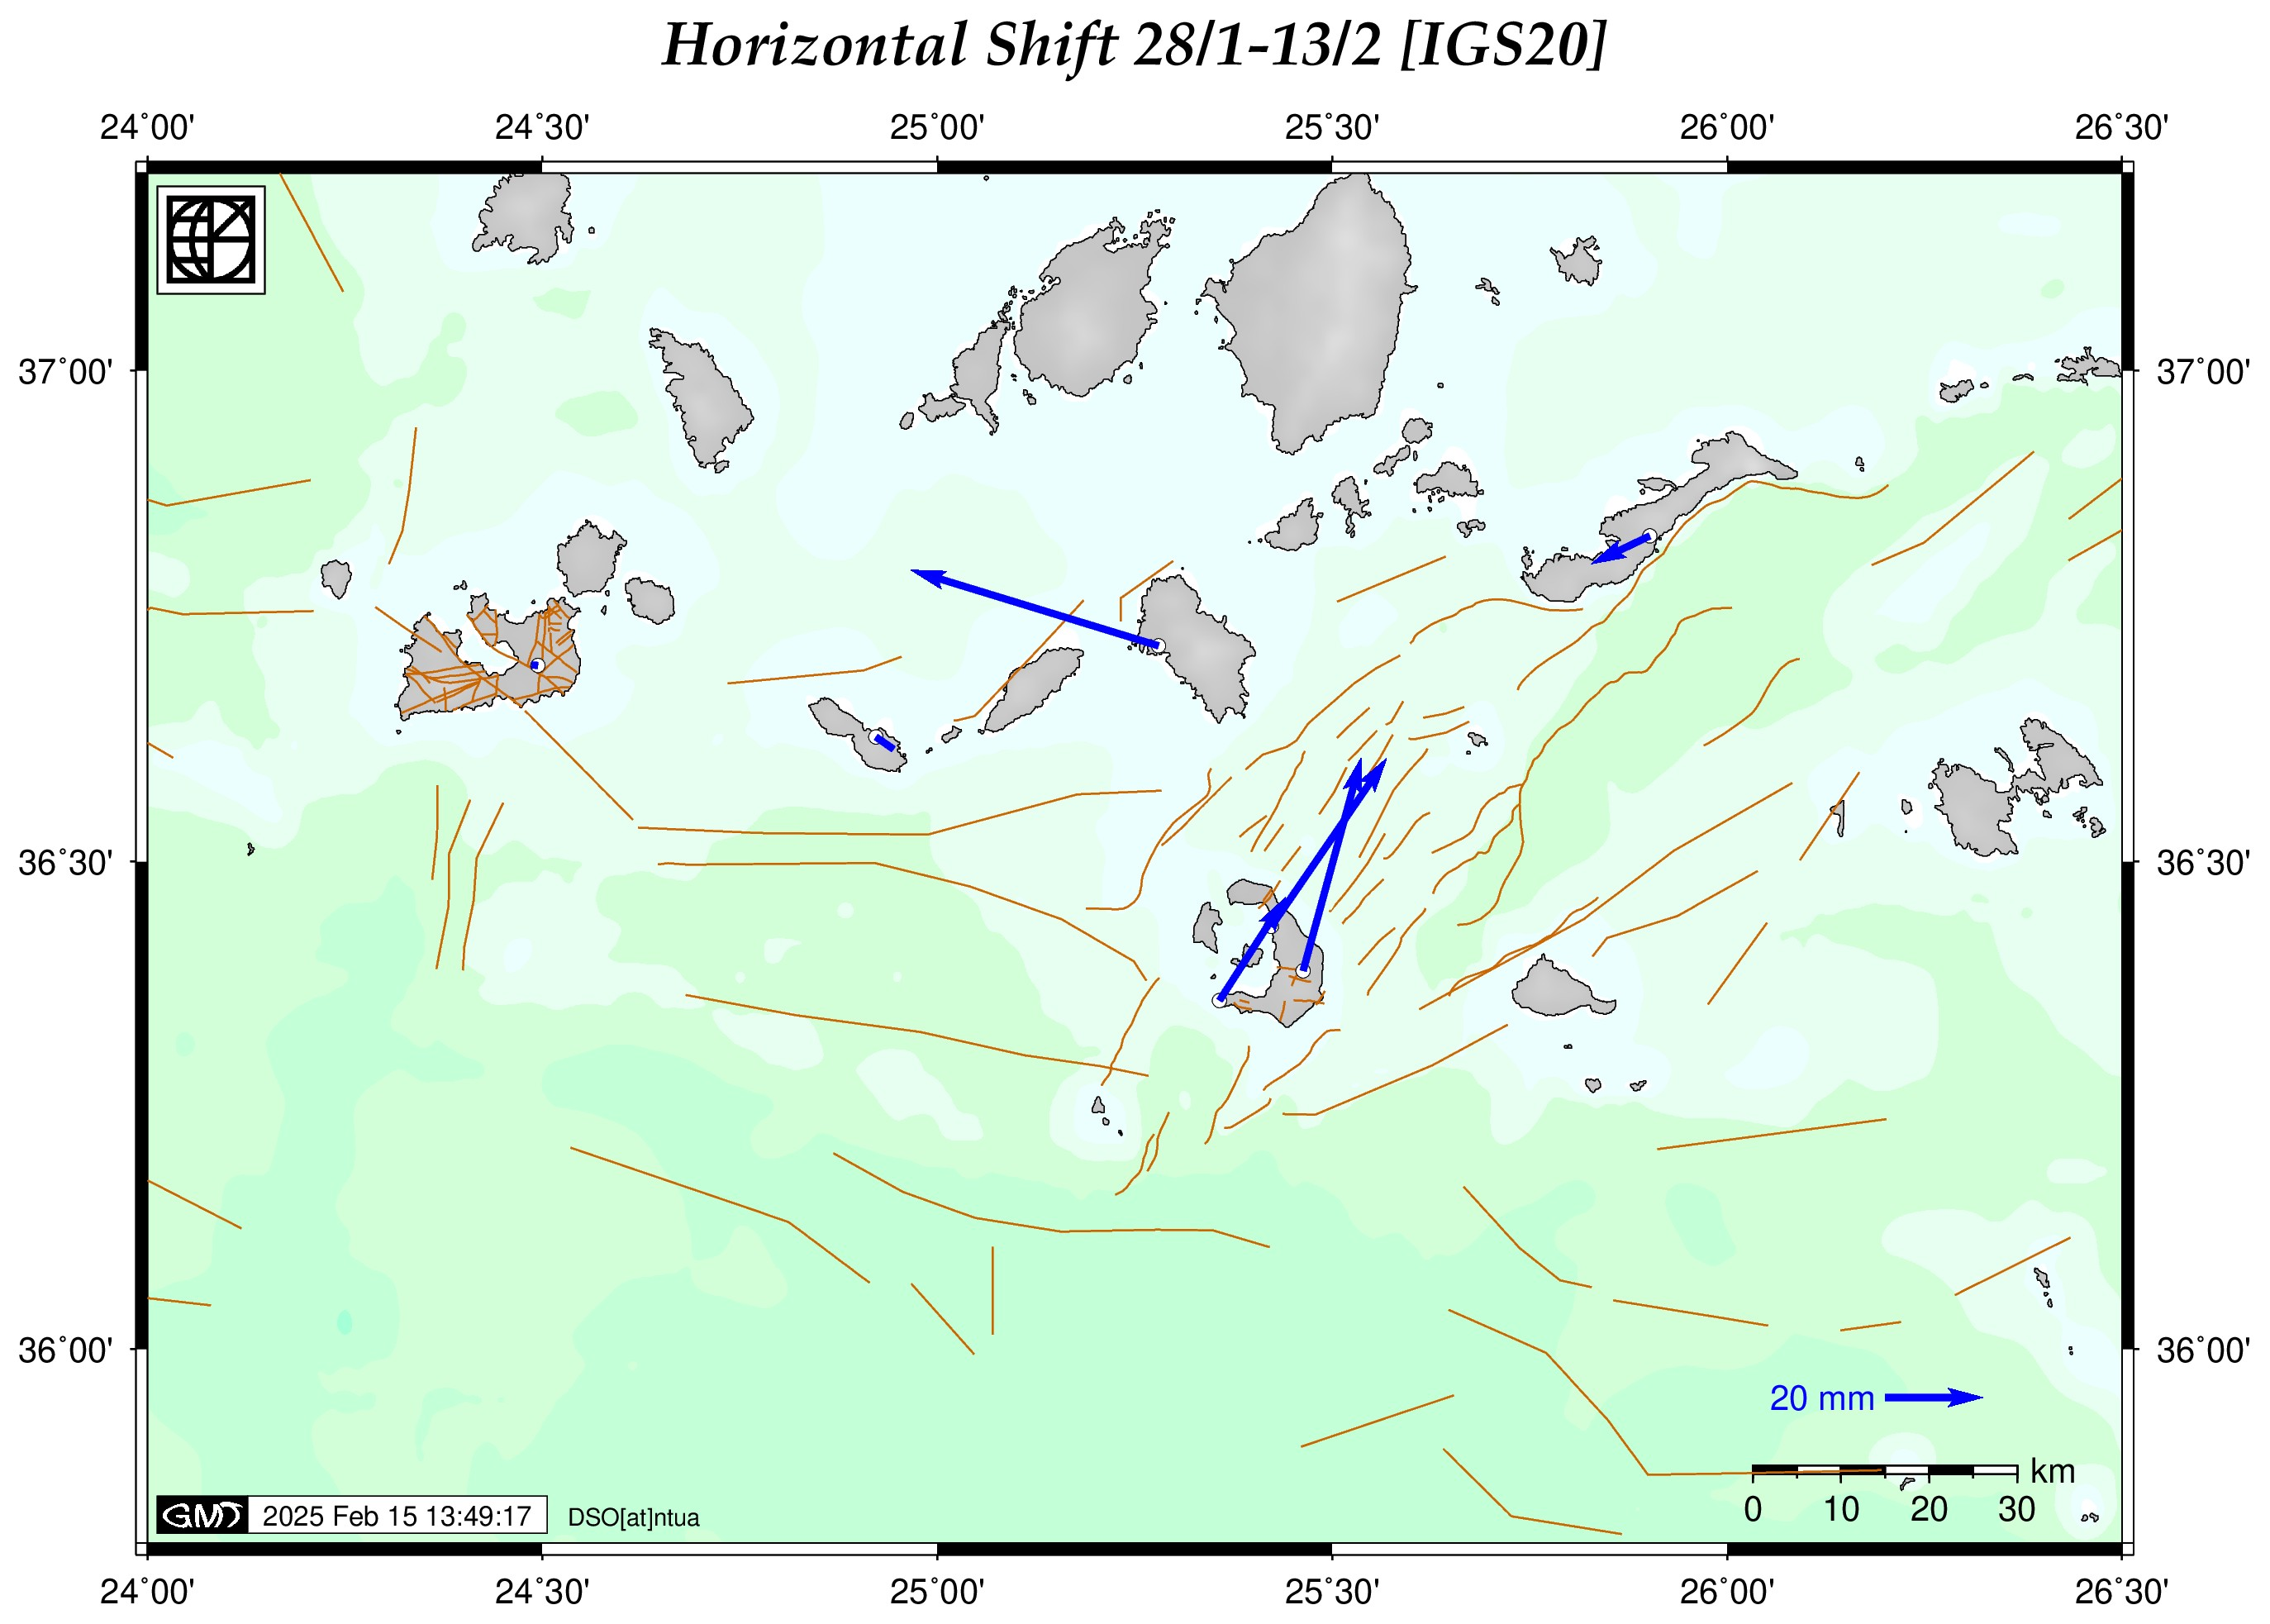
\includegraphics[width=.97\textwidth]{sant_2501_vhor01.jpg}
      \end{center}  
    \end{column}
    \begin{column}{.5\textwidth}
      \begin{center}
        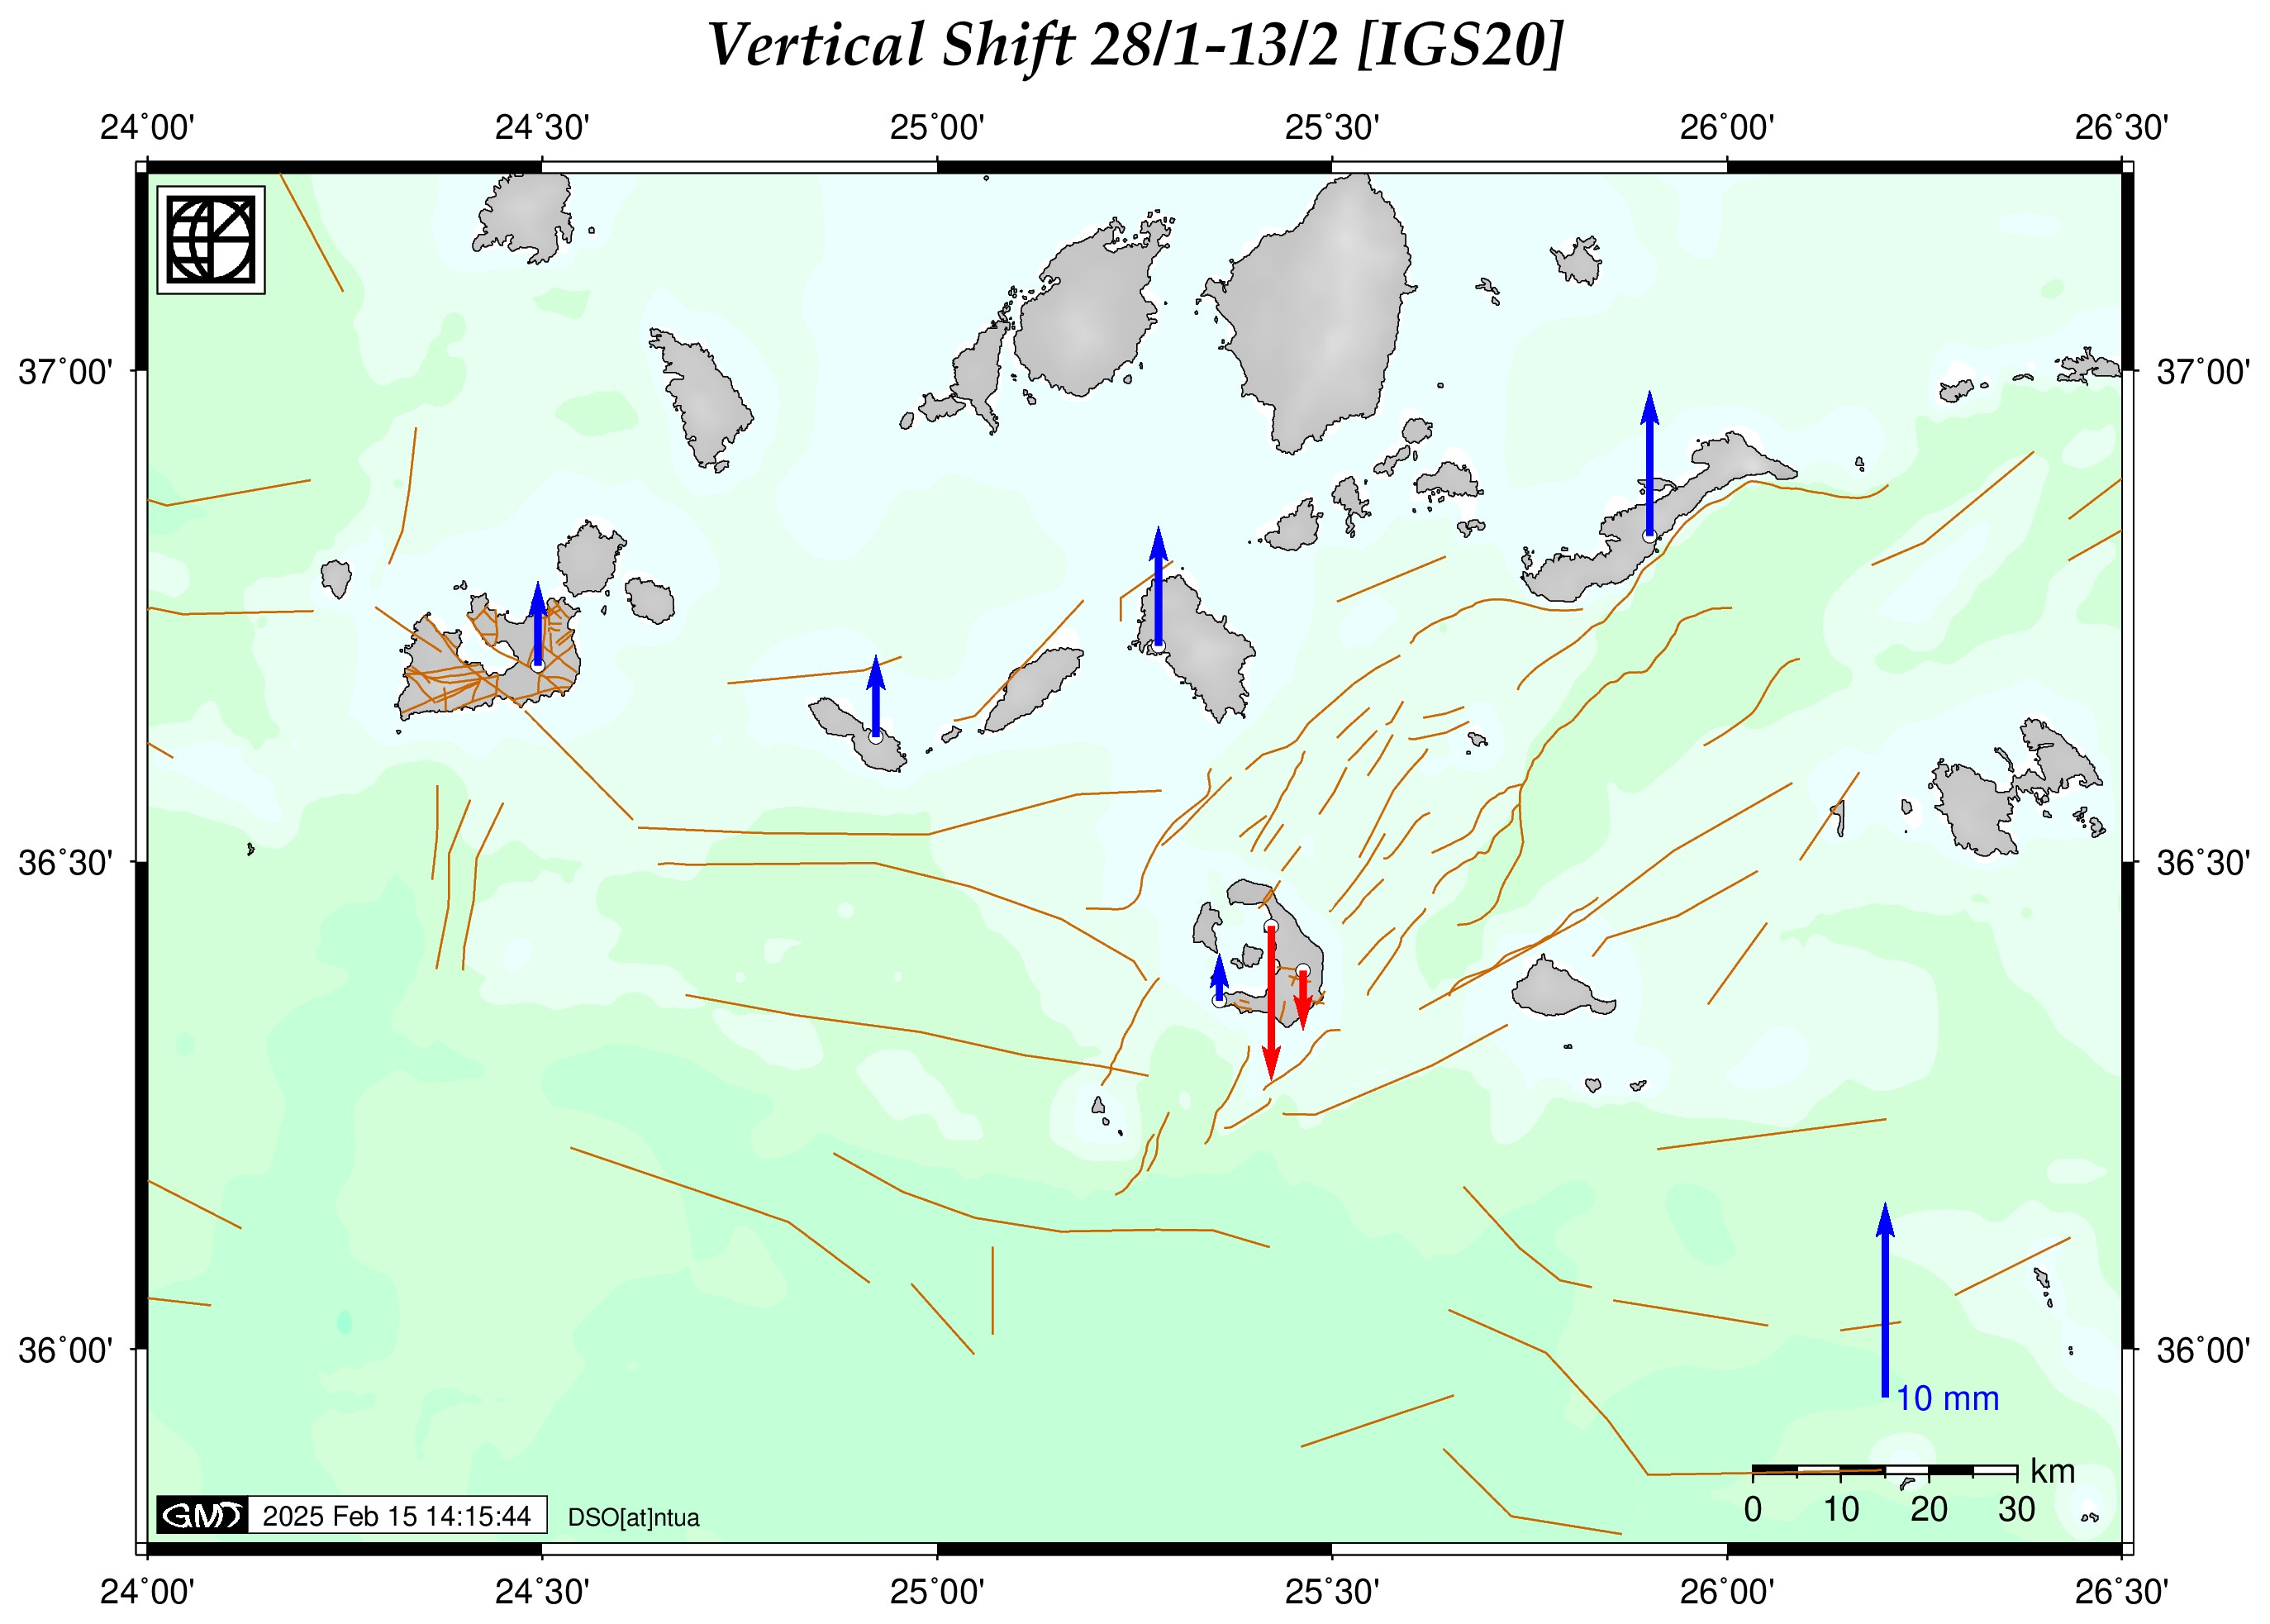
\includegraphics[width=.97\textwidth]{sant_2501_vver01.jpg}
      \end{center}       
    \end{column}
  \end{columns}  

\end{frame}
\note{}

 % ------------------------------------------------------------------------------
\begin{frame}
  \frametitle{Λειτουργία σταθμών}
  \framesubtitle{}
  \label{}
  \vskip-1cm
  \begin{columns}[T]
    \begin{column}{.25\textwidth}
      \begin{center}
      {\scriptsize SNTR 12653M001}
        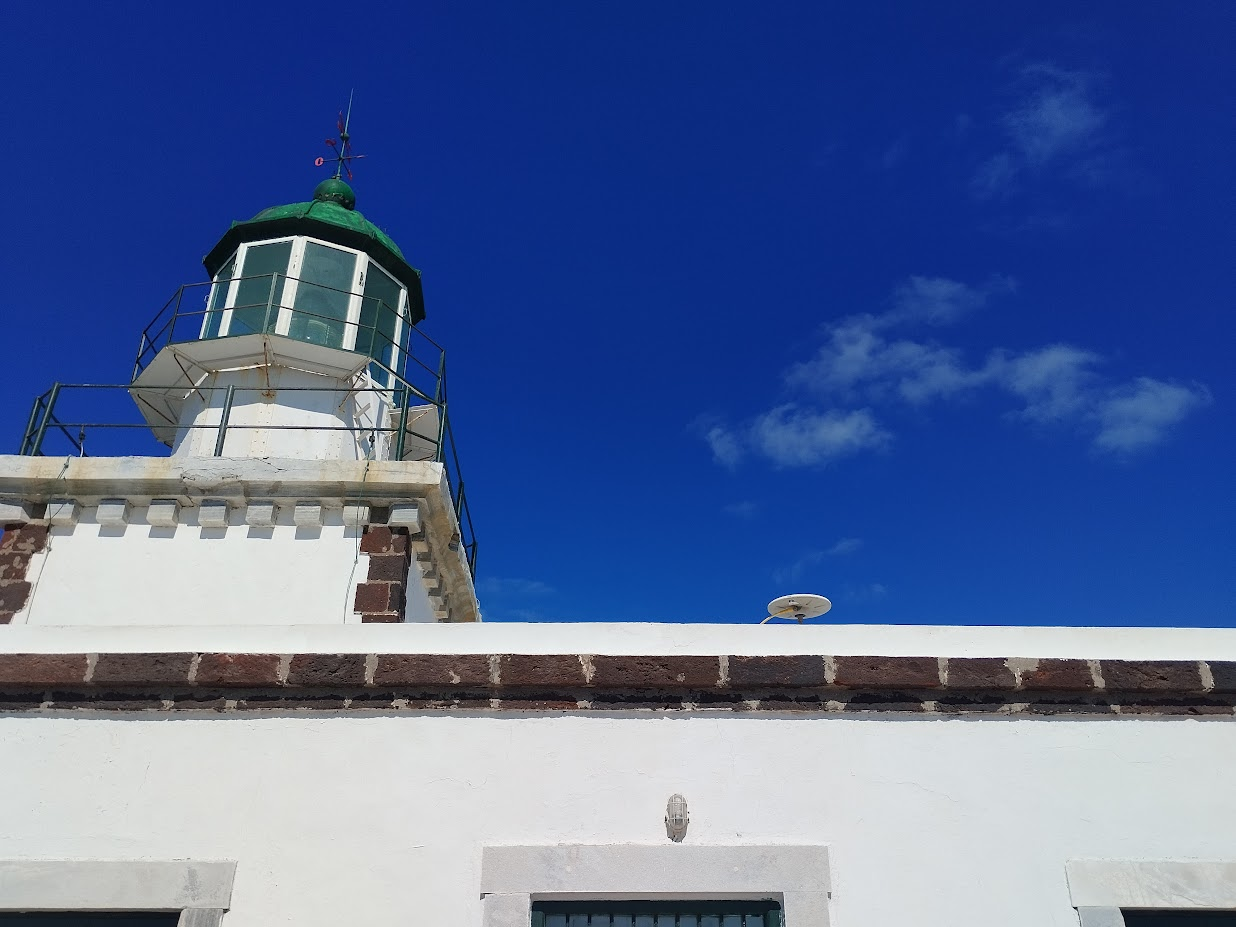
\includegraphics[width=.97\textwidth]{SNTR_01.jpg}
      \end{center}  
    \end{column}
    \begin{column}{.25\textwidth}
      \begin{center}
       {\scriptsize WNRY 12687M001}
        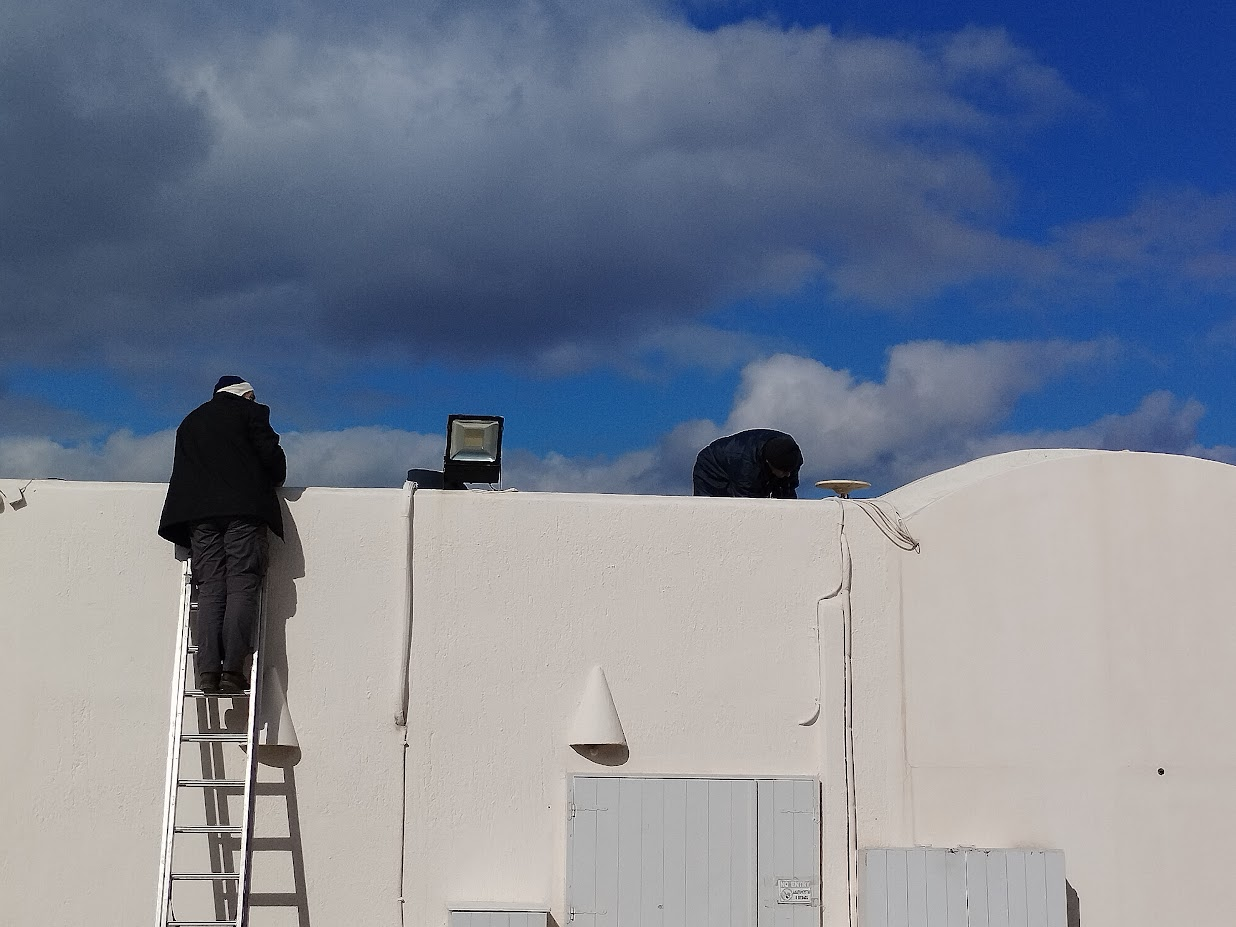
\includegraphics[width=.97\textwidth]{wnry_01.jpg}
      \end{center}       
    \end{column}
  \begin{column}{.25\textwidth}
      \begin{center}
       {\scriptsize NOMI}
        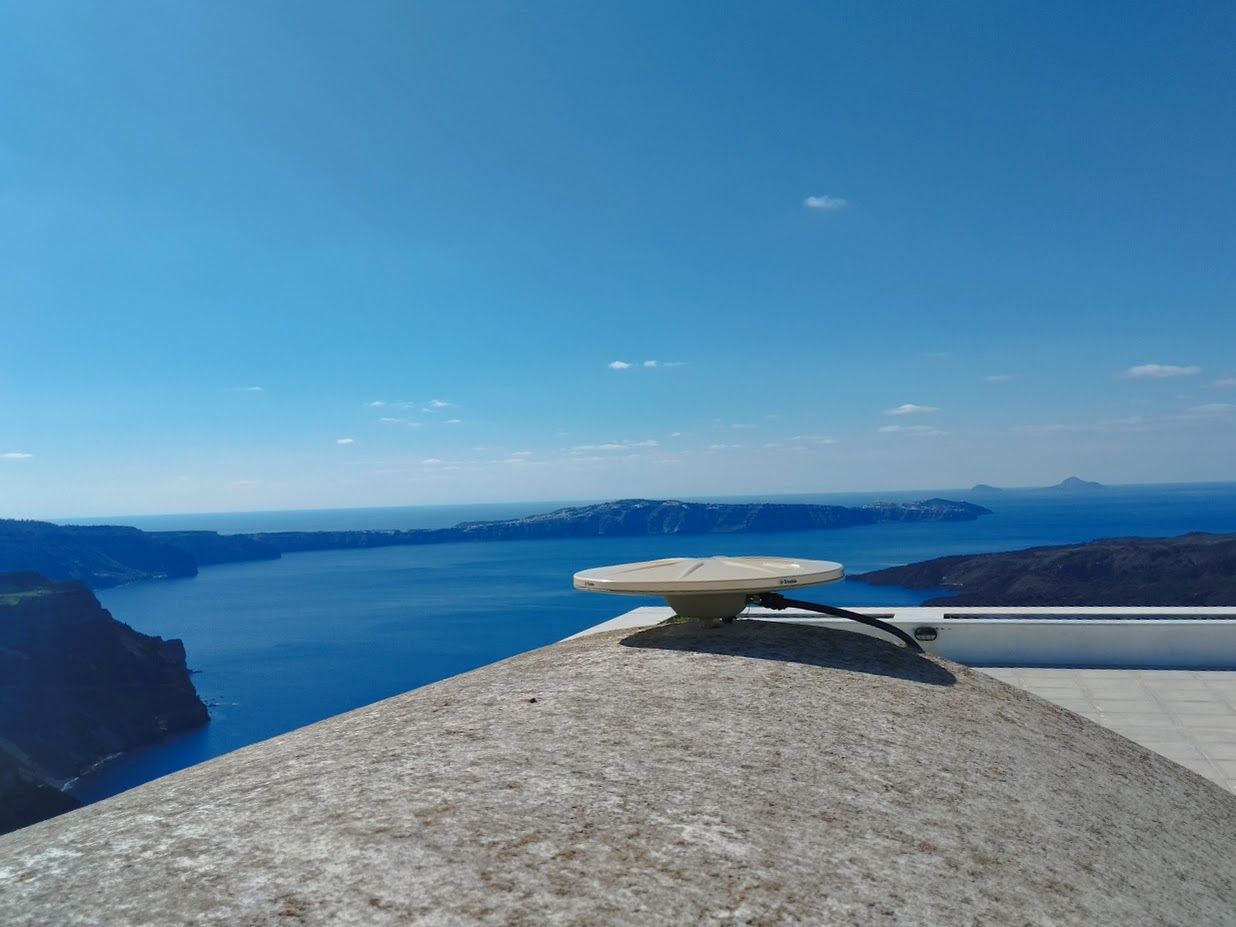
\includegraphics[width=.97\textwidth]{NOMI_01.jpg}
      \end{center}  
    \end{column}
    \begin{column}{.25\textwidth}
      \begin{center}
       {\scriptsize Campaign}
        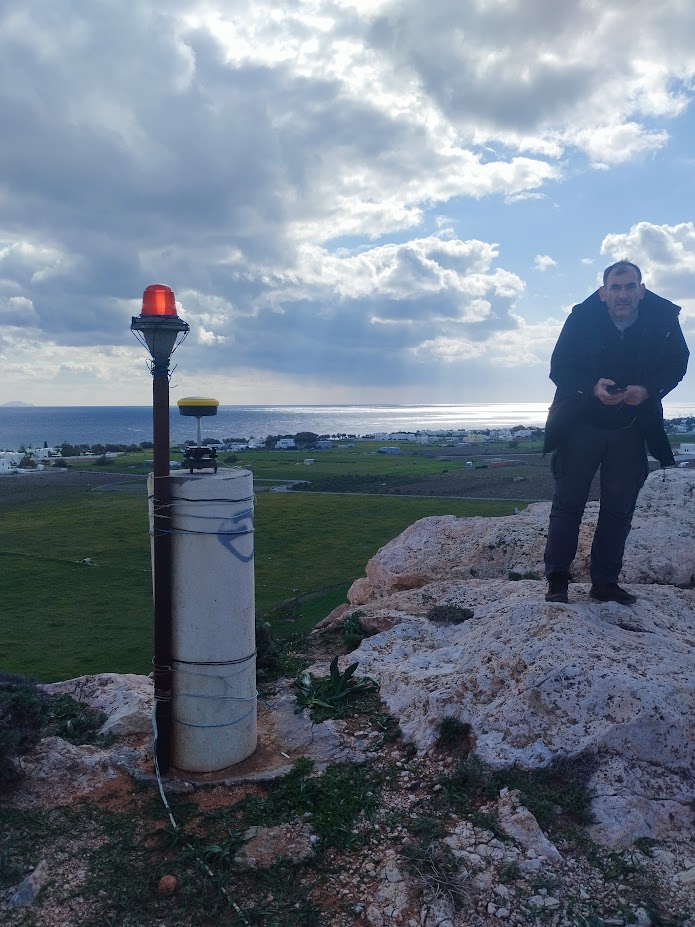
\includegraphics[width=.7\textwidth]{sn_camp.jpg}
      \end{center}       
    \end{column}
  \end{columns}  
  ~\\[1em]
\begin{scriptsize}
- Διάθεση δεδομένων: \url{http://dionysos.survey.ntua.gr/dsoportal/\_datacenter/httpdata.html}\\
- Ο σταθμός ΝΟΜΙ είναι σε συνεργασία με το Πανεπιστήμιο Πατρών και την άδεια του EarthScope.
\end{scriptsize}

\end{frame}
\note{}

 % ------------------------------------------------------------------------------
\begin{frame}
  \frametitle{Διάθεση δεδομένανων/αποτελεσμάτων}
  \framesubtitle{}
  \label{}
  \vskip-1.2cm
\begin{center}
  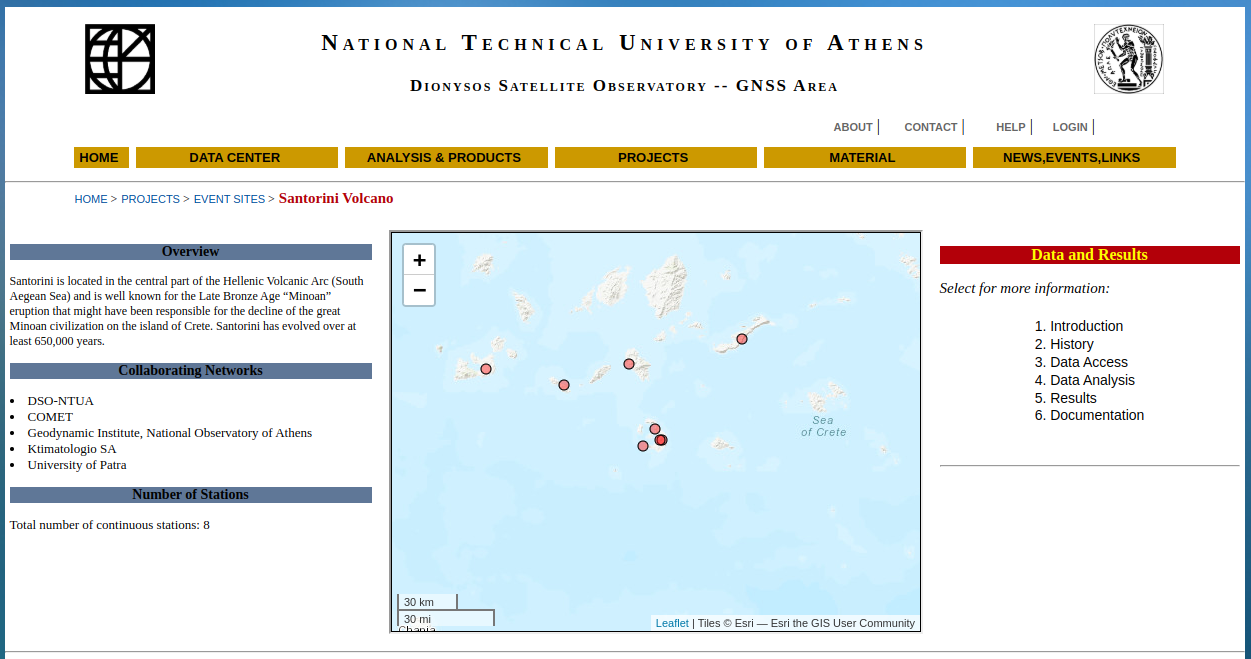
\includegraphics[width=.8\textwidth]{dsoportal_sant.png}
\end{center}
\url{http://dionysos.survey.ntua.gr/dsoportal/\_projects/supersites/santorini/}
\end{frame}
\note{}

%%-----------------------------------------------------------------------------
%% END OF PRESENTATION ...
%%-----------------------------------------------------------------------------

% ************************  Thank you frame  **********************************
% include Thank U last frame
\makethanku % Ιncluded to class file

% ************************  Bibliography  *************************************
% % % Add 'printbib' option in Class file to Include Bibliography
\ifdefinePrintbib
  \begin{frame}[t,allowframebreaks]
    \frametitle{References}
    \printbibliography
  \end{frame}
\fi

% ************************  Cut Frames  **************************************
% Add back up cut frames
% % \section{Κομμένα}

\graphicspath{{Chapter2/Figs/Vector/}}

% ----------------------------------------------------------------------------
% % CHAPTER 2
%-----------------------------------------------------------------------------

\begin{frame}
  \frametitle{Back frames}
  \label{frcut:backframes}

Πρόσθεσε εδώ frames σαν παράρτημα τη παρουσίασης στη περίπτωση που χρειαστούν κατά τη διάρκεια της ομιλίας.

\end{frame}
\note{}













% *********************** end of document ************************************
\end{document}
